% \documentclass[14pt, a4paper]{extarticle}
%
% \usepackage{listings}
%
% \usepackage[paper=A4]{typearea}
% \usepackage{lipsum}
%
% \usepackage{graphicx}
% \graphicspath{{./images/}}
% \DeclareGraphicsExtensions{.jpg,.png}
% \usepackage{csvsimple}
%
% \usepackage{amsfonts}
% \usepackage{amsmath}
% \usepackage[english,russian]{babel}
%
% \usepackage{fontspec} 
% \usepackage{unicode-math}
% \defaultfontfeatures{Ligatures={TeX},Renderer=Basic}
% \setmainfont[Ligatures={TeX,Historic}]{Times New Roman}
% \setmonofont{Courier New}
% %\setmathfont{XITSMath-Regular}
% %\newfontfamily\cyrillicfonttt[Script=Cyrillic]{Courier New}
%
% \usepackage{xcolor}
%
% \usepackage{array}
% \newcommand\ChangeRT[1]{\noalign{\hrule height #1}}
%
% \usepackage{tabularx}
% \newcolumntype{s}{>{\raggedright\arraybackslash}X}
% %\renewcommand{\tabularxcolumn}[1]{m{#1}} % Вертикальное центрирование текста
%
% \usepackage{indentfirst} %отступ первой строки первого абзаца
% \linespread{1.25}
%
% \setlength{\footskip}{1cm}
% \usepackage{geometry}
% \geometry{left=3cm}
% \geometry{right=1cm}
% \geometry{top=2cm}
% \geometry{bottom=2cm}
%
% \setlength{\parindent}{1.25cm}
%
% \usepackage{enumitem}
% \setlist{left=\parindent, labelsep=1cm, itemsep=0pt, topsep=0pt}
%
% \usepackage[final]{pdfpages}
%
% \usepackage{titlesec} % оформление заголовков
%
% \titleformat{\section}[block]
% 	{\bfseries\fontsize{18pt}{21.6pt}\selectfont}
%         {\thesection}
%         {1em}{}
% \titleformat{name=\section,numberless}[block]
% 	{\centering\bfseries\fontsize{18pt}{21.6pt}\selectfont}
%         {}
%         {0em}{}{}
% \titlespacing{\section}
%  {\parindent}% space at the left
%  {0em}% space before
%  {10mm}% space after
% \titleformat{\subsection}[block]
% 	{\bfseries\hspace{\parindent}\fontsize{16pt}{19.2pt}\selectfont}
%         {\thesubsection}
%         {1em}{}
%
% % Отображать только заголовки первого уровня
% %\setcounter{tocdepth}{1}
%
% \usepackage{etoolbox}
%
% \usepackage{nameref}
%
% \usepackage{xurl}
% \usepackage{hyperref}
% \hypersetup{
%     colorlinks,
%     citecolor=black,
%     filecolor=black,
%     linkcolor=black,
%     urlcolor=black,
%     breaklinks=true
% }
% \urlstyle{same}
%        
% \usepackage{float}
% \usepackage{caption}
%
% \usepackage{newfloat}
% \DeclareCaptionType[name=Листинг, placement=htbp]{listing}
%
% \usepackage{fancyvrb}
%
% \DeclareCaptionLabelSeparator{emdash}{\;\textemdash\;}
% \captionsetup[figure]{name={Рисунок}, labelsep=emdash, justification=centering, position=above, singlelinecheck=off, font={small, bf}, labelfont=bf, skip=6pt}
% \captionsetup[table]{name={Таблица}, labelsep=emdash, justification=raggedright, position=top, singlelinecheck=off, font={small, it}, labelfont=it, skip=6pt, margin=0.6cm}
% \captionsetup[listing]{name={Листинг}, labelsep=emdash, justification=raggedright, position=top, singlelinecheck=off, font={small, it}, labelfont=it, skip=-16pt, margin=0.6cm}
% \captionsetup[lstlisting]{labelsep=emdash, justification=raggedright, position=top, singlelinecheck=off, font={small, it}, labelfont=it, skip=6pt, margin=0cm}
%
% % Нумерация по разделам
% \counterwithin{figure}{section}
% \counterwithin{table}{section}
% \counterwithin{listing}{section}
%
% \usepackage{ragged2e}
% \usepackage{microtype}
%
% \justifying
% \tolerance=500
% \hyphenpenalty=10000 % отключение переноса
% \emergencystretch=3em
%
% \usepackage{setspace}
%
% \usepackage{multirow}
%
% \usepackage[
% citestyle=gost-numeric,
% style=gost-numeric, 
% blockpunct=emdash,
% backend=biber,
% sorting=none
% ]{biblatex}
%
% \defcounter{biburlnumpenalty}{3000}
% \defcounter{biburlucpenalty}{6000}
% \defcounter{biburllcpenalty}{9000}
%
% \DeclareFieldFormat{url}{Режим доступа: #1}
% \DeclareFieldFormat{urldate}{(Дата обращения: #1)}
% \renewcommand*{\entrysetpunct}{\par\nopunct\!\!}
%
%
% \defbibheading{bibliography}[\bibname]{%
%   \section*{\centering #1}%
%   \markboth{#1}{#1}}
%
% \addbibresource{misc/thesis5.bib}
%
% \usepackage{pdflscape}
% \usepackage{everypage}
%
% \newcommand{\Lpagenumber}{\ifdim\textwidth=\linewidth\else\bgroup
%   \dimendef\margin=0 %use \margin instead of \dimen0
%   \ifodd\value{page}\margin=\oddsidemargin
%   \else\margin=\evensidemargin
%   \fi
%   \raisebox{\dimexpr-\topmargin-\headheight-\headsep-0.5\linewidth}[0pt][0pt]{%
%     \rlap{\hspace{\dimexpr-\margin+\textheight+\footskip}%
%     \llap{\rotatebox{90}{\thepage}}}}%
% \egroup\fi}
% \AddEverypageHook{\Lpagenumber}%
%
% \usepackage{tocloft}
% \setlength{\cftsecnumwidth}{0pt}
% \setlength{\cftsecindent}{0pt}% Remove indent for \section
% \setlength{\cftsubsecindent}{0pt}% Remove indent for \subsection
% \setlength{\cftsubsubsecindent}{0pt}% Remove indent for \subsubsection
% \setlength{\cftbeforesecskip}{0pt}% Change spacing between sections
% \renewcommand{\cftsecaftersnumb}{\hspace{1.5em}}
% \renewcommand{\cftsecleader}{\cftdotfill{\cftdotsep}}
% \renewcommand{\cftdotsep}{1.25}
% \renewcommand{\cftsecfont}{\normalfont}
% \renewcommand{\cftsecpagefont}{\normalfont}
% \renewcommand{\cfttoctitlefont}{\hfil \bfseries \large}
%
% % Поддержка листингов
% \usepackage{listings}
% \lstdefinestyle{gost}{
%     basicstyle=\ttfamily\footnotesize,
%     breakatwhitespace=false,
%     breaklines=true,
%     keepspaces=true,
%     showspaces=false,          
%     showstringspaces=false,
%     frame=single
% }
% \lstset{style=gost}
%
% \usepackage{lipsum} 
%
% \begin{document}
%
% \pretocmd{\section}{\newpage}{}{}
%
% \def\contentsname{СОДЕРЖАНИЕ}
%
% \pagenumbering{gobble}
% \begin{titlepage}
% \includepdf[pages=-]{misc/Gostev}
% \end{titlepage}
% \pagenumbering{arabic}
% \setcounter{page}{4}
% \tableofcontents
%

\documentclass[14pt, a4paper]{extarticle}
% Русская локализация
\usepackage[english,russian]{babel}

% Использование математических шрифтов
\usepackage{unicode-math}

% Шрифты
\usepackage{fontspec}
\usepackage{courier}
\defaultfontfeatures{Ligatures={TeX},Renderer=Basic}
\setmainfont[Ligatures={TeX}]{Times New Roman}
\setmonofont{Courier New}
\setmathfont{XITS Math}

% Расширенные ссылки
\usepackage{nameref}

% Оформление URL
\usepackage{xurl}
\usepackage{hyperref}
\hypersetup{
    colorlinks,
    citecolor=black,
    filecolor=black,
    linkcolor=black,
    urlcolor=black,
    breaklinks=true,
}
\urlstyle{same}

% Поддержка изображений
\usepackage{graphicx}
\graphicspath{{./images/}}
\DeclareGraphicsExtensions{.jpg,.png}

% Таблицы
\usepackage{tabularx}
\usepackage{tabulary}
\usepackage{multirow}
\usepackage{hhline} 
% Выравнивание по левому краю, с многострочностью
\newcolumntype{s}{>{\raggedright\arraybackslash}X}

% Поддержка листингов
\usepackage{listings}
\lstdefinestyle{gost}{
    basicstyle=\ttfamily\footnotesize,
    breakatwhitespace=false,
    breaklines=true,
    keepspaces=true,
    showspaces=false,          
    showstringspaces=false,
    frame=single
}
\lstset{style=gost}%

% Отступ первой строки первого абзаца
\usepackage{indentfirst}
\linespread{1.25}

% Размер полей в документе
\usepackage{geometry}
\geometry{left=3cm}
\geometry{right=1cm}
\geometry{top=2cm}
\geometry{bottom=2cm}

% Абзацный отступ
\setlength{\parindent}{1.25cm}

% Отступ для элементов в списке
\usepackage{enumitem}
\setlist{left=\parindent, labelsep=1cm, itemsep=0pt, topsep=0pt}

% Загрузка pdf-документов (нужно для титульников)
\usepackage[final]{pdfpages}
% Возможность поворота pdf файло
\usepackage{pdflscape}
\usepackage{everypage}

\newcommand{\Lpagenumber}{\ifdim\textwidth=\linewidth\else\bgroup%
  \dimendef\margin=0 %use \margin instead of \dimen0
  \ifodd\value{page}\margin=\oddsidemargin
  \else\margin=\evensidemargin%
  \fi
  \raisebox{\dimexpr-\topmargin-\headheight-\headsep-0.5\linewidth}[0pt][0pt]{%
    \rlap{\hspace{\dimexpr-\margin+\textheight+\footskip}%
    \llap{\rotatebox{90}{\thepage}}}}%
\egroup\fi}
\AddEverypageHook{\Lpagenumber}%

\usepackage{float}
% Форматирование подписей
\usepackage{caption}

\usepackage{newfloat}

\DeclareCaptionLabelSeparator{emdash}{\;\textemdash\;}
\captionsetup[figure]{name={Рисунок}, labelsep=emdash, justification=centering, position=above, singlelinecheck=off, font={small, bf}, labelfont=bf, skip=6pt}
\captionsetup[table]{name={Таблица}, labelsep=emdash, justification=raggedright, position=top, singlelinecheck=off, font={small, it}, labelfont=it, skip=6pt, margin=0cm}
\captionsetup[lstlisting]{labelsep=emdash, justification=raggedright, position=top, singlelinecheck=off, font={small, it}, labelfont=it, skip=6pt, margin=0cm}
%%%%%%%%%%%%%%%%%%%%%%%%%%%%%%%%%%%%%%% ТО ЧТО НАПИСАНО У ЖЕКИ ПРО ЛИСТИНГИ
% \captionsetup[lstlisting]{labelsep=emdash, 
%                           justification=raggedright, 
%                           position=top, 
%                           singlelinecheck=off, 
%                           font={singlespacing, small, it}, 
%                           labelfont=it, 
%                           skip=0pt, 
%                           margin=0cm}
%
% % Поддержка листингов
% \usepackage{listings}
% \lstdefinestyle{gost}{
%     basicstyle=\ttfamily\fontsize{10pt}{10pt}\linespread{1}\selectfont,
%     breakatwhitespace=false,
%     breaklines=true,
%     keepspaces=true,
%     showspaces=false,          
%     showstringspaces=false,
%     frame=single
% }
% \lstset{style=gost}
%
% \usepackage{lipsum}
%%%%%%%%%%%%%%%%%%%%%%%%%%%%%%%%%%%%%%%%%%%%%%%%%%

% Задаю нормальное название листингу 
\renewcommand\lstlistingname{Листинг}

% Нумеровать внутри заголовков первого уровня
\counterwithin{figure}{section}
\counterwithin{table}{section}
%\counterwithin{lstlisting}{section}
\AtBeginDocument{\counterwithin{lstlisting}{section}}

% Отключение переносов текста
\usepackage{ragged2e}
\justifying
\tolerance=500
\hyphenpenalty=10000
\emergencystretch=3em

% Форматирование заголовков
\usepackage{titlesec}
% Оформление заголовка первого уровня
% Полужирное начертание
% Кегль 18 пт
% С новой страницы
\titleformat{\section}[block]
	{\newpage\bfseries\fontsize{18pt}{21.6pt}\selectfont}
        {\thesection}
        {1em}{}
% Оформление ненумерованных заголовков (Введение, Содержание, список источников, и.т.д.)
\titleformat{name=\section,numberless}[block]
	{\centering\newpage\bfseries\fontsize{18pt}{21.6pt}\selectfont}
        {}
        {0em}{}{}
% Отступы у заголовков первого уровня
\titlespacing{\section}
 {\parindent}% отступ слева (равен 1.25 см, как у отступа первой строки абзаца)
 {0em}% интервал перед
 {10mm}% интервал после
% Оформление заголовков второго уровня
\titleformat{\subsection}[block]
	{\bfseries\fontsize{16pt}{19.2pt}\selectfont}
        {\thesubsection}
        {1em}{}
% Отступы у заголовков второго уровня
\titlespacing{\subsection}
 {\parindent}% пробел слева
 {15mm}% отступ перед
 {10mm}% отступ после
% Оформление заголовков второго уровня
\titleformat{\subsubsection}[block]
	{\bfseries\selectfont}
        {\thesubsection}
        {1em}{}
% Отступы у заголовков второго уровня
\titlespacing{\subsubsection}
 {\parindent}% пробел слева
 {15mm}% отступ перед
 {10mm}% отступ после

% Оформление заголовков в содержании
\usepackage{titletoc}
\contentsmargin{0pt}
\renewcommand\contentspage{\thecontentspage}
\dottedcontents{section}[2.3em]{}{2.3em}{5pt}
\dottedcontents{subsection}[2.3em]{}{2.3em}{5pt}
% Оформление приложений
\usepackage{appendix}
\renewcommand\appendixpagename{ПРИЛОЖЕНИЯ}

% Подключение biblatex, с использованием стиля gost-numeric
\usepackage[
citestyle=gost-numeric,
style=gost-numeric, 
blockpunct=emdash,
backend=biber,
sorting=none
]{biblatex}
% Запрет разрыва url ссылок
\defcounter{biburlnumpenalty}{3000}
\defcounter{biburlucpenalty}{6000}
\defcounter{biburllcpenalty}{9000}
% Добавление полей для ссылок и даты обращения к ним
\DeclareFieldFormat{url}{Режим доступа: #1}
\DeclareFieldFormat{urldate}{(Дата обращения: #1)}
\renewcommand*{\entrysetpunct}{\par\nopunct\!\!}
% Использовать prac.bib как источник
\addbibresource{preamble.bib}
% Форматирование заголовка библиографии
\defbibheading{bibliography}[\bibname]{%
  \section*{\centering #1}%
  \markboth{#1}{#1}}

\usepackage{appendix}

% \def\Asbuk#1{\expandafter\russian@Alph\csname c@#1\endcsname}
% \if@uni@ode
% 	\def\russian@Alph#1{\ifcase#1\or
% 		А\or Б\or В\or Г\or Д\or Е\or Ж\or
% 		З\or И\or К\or Л\or М\or Н\or О\or
% 		П\or Р\or С\or Т\or У\or Ф\or Х\or
% 		Ц\or Ч\or Ш\or Щ\or Э\or Ю\or Я\else\@ctrerr\fi}
% \else
% 	\def\russian@Alph#1{\ifcase#1\or
% 		\CYRA\or\CYRB\or\CYRV\or\CYRG\or\CYRD\or\CYRE\or\CYRZH\or
% 		\CYRZ\or\CYRI\or\CYRK\or\CYRL\or\CYRM\or\CYRN\or\CYRO\or
% 		\CYRP\or\CYRR\or\CYRS\or\CYRT\or\CYRU\or\CYRF\or\CYRH\or
% 		\CYRC\or\CYRCH\or\CYRSH\or\CYRSHCH\or\CYREREV\or\CYRYU\or
% 		\CYRYA\else\@ctrerr\fi}
% \fi
\makeatletter
\newcommand{\realasbuk}[1]{\expandafter\russian@realAlph\csname c@#1\endcsname}

\def\russian@realAlph#1{\ifcase#1\or
   А\or Б\or В\or Г\or Д\or Е\or Ж\or
   З\or И\or К\or Л\or М\or Н\or О\or
   П\or Р\or С\or Т\or У\or Ф\or Х\or
   Ц\or Ч\or Ш\or Щ\or Э\or Ю\or Я\else\xpg@ill@value{#1}{russian@Alph}\fi}
\def\russian@realalph#1{\ifcase#1\or
   а\or б\or в\or г\or д\or е\or ж\or
   з\or и\or к\or л\or м\or н\or о\or
   п\or р\or с\or т\or у\or ф\or х\or
   ц\or ч\or ш\or щ\or э\or ю\or я\else\xpg@ill@value{#1}{russian@alph}\fi}

\AddEnumerateCounter{\realasbuk}{\russian@realAlph}{щ}
\makeatother

\usepackage{lipsum}
\begin{document}
\def\contentsname{СОДЕРЖАНИЕ}

% Загрузка титула
\pagenumbering{gobble}
\begin{titlepage}
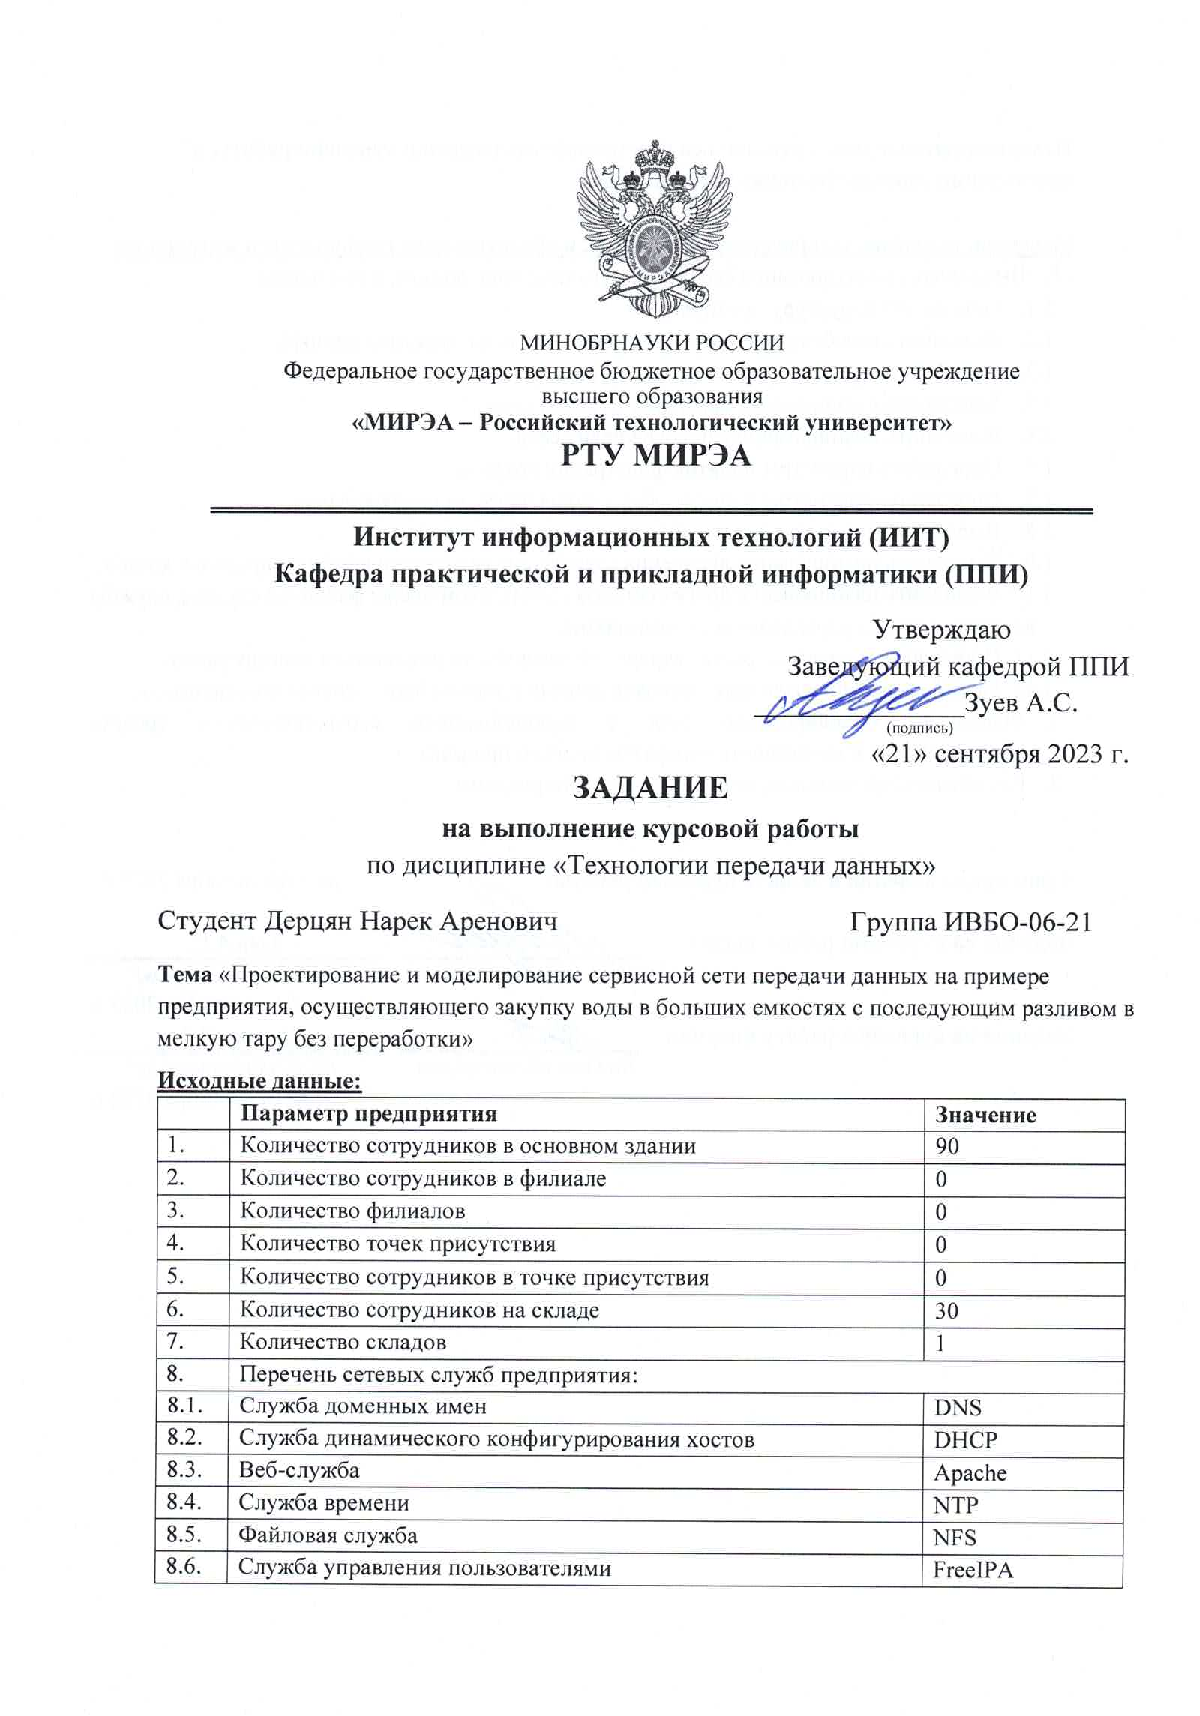
\includepdf[pages={1-2}]{../misc/title.pdf}
\end{titlepage}
\pagenumbering{arabic}
\setcounter{page}{3}
% Содержание
\tableofcontents

\clearpage
\section*{ВВЕДЕНИЕ}
%%% start Актуальность темы
В современном мире технологии сервисной передачи данных играют значительную роль в повседневной жизни и деятельности организаций. В частности, для предприятий, осуществляющих закупку воду в больших емкостях и последующий разлив в мелкие тары без переработки, эффективная сервисная сеть передачи данных является важным условием успешной и стабильной работы.

Актуальность данной темы обусловлена быстрым ростом объемов передаваемой информации и необходимостью внедрения современных технологий в процессе проектирования сервисных сетей передачи данных. Важность исследования заключается в возможности определения оптимального подхода к проектированию сервисной сети передачи данных для улучшения эффективности работы предприятия.

Объектом исследования является сервисная сеть передачи данных, предметом исследования --- особенности проектирования и реализации сервисной сети передачи данных на примере предприятия, занимающегося закупкой и разливом воды. Цель работы состоит в планировании и реализации сервисной сети передачи данных, обеспечивающей эффективное функционирование предприятия.

Для достижения поставленной цели, в рамках работы предполагается решение следующих задач:

\begin{enumerate}
        \item Проанализировать исходные данные в поставленной задаче;
        \item Провести планирование адресации и маршрутизации сети передачи данных, разделение на виртуальные и локальные сети;
        \item Провести прототипирование сети передачи данных;
        \item Выполнить планирование таких служб, как файловая, служба времени, службы управления пользователями;
		\item Провести расчет сервисной нагрузки по результатам планирования;
        \item Провести настройку и тестирование сети передачи данных.
\end{enumerate}

Инструментальными средствами исследования выступают программные инструменты, такие как Cisco Packet Tracer, Apache, которые позволяют моделировать и тестировать сетевые архитектуры.

Основными источниками информации для работы станут научные публикации, учебники и интернет-ресурсы, посвященные технологиям передачи данных, сетевому проектированию и планированию.

Основное содержание работы будет состоять из следующих разделов:

\begin{enumerate}
    \item Обзор теоретических основ и современных технологий передачи данных, их применение в процессе проектирования сетей для предприятий различных масштабов и отраслей;
    \item Изучение специфики деятельности предприятия, анализ требований к сети сервисной передачи данных;
    \item Разработка схемы адресации и маршрутизации сети передачи данных с учетом исходных данных и требований предприятия;
    \item Проектирование виртуальных и локальных сетей для оптимального разделения и обеспечения безопасности передачи данных;
    \item Создание прототипа сети передачи данных с использованием инструментария Cisco Packet Tracer для проверки корректности проектирования и определения возможных узких мест и проблем;
    \item Выполнение планирования файловых сетевых, служб времени, служб управления пользователями;
    \item Настройка и тестирование сети сервисной передачи данных на предприятии, оценка ее работоспособности и эффективности;
	\item Проведение расчетов для определения сервисной нагрузки по результатам планирования;
    \item Разработка рекомендаций по улучшению процесса проектирования сетей передачи данных и дальнейшего развития инфраструктуры предприятия.
\end{enumerate}

В результате проведенного исследования, будет предложено оптимальное решение по проектированию сети сервисной передачи данных для предприятия, осуществляющего закупку и разлив воды, что позволит обеспечить стабильную работу в долгосрочной перспективе.

\section*{СОКРАЩЕНИЯ}
\addcontentsline{toc}{section}{СОКРАЩЕНИЯ} % это чтобы в содержании отображалось
\begin{raggedright}
АРМ --- Автоматизированное Рабочее Место \\
VLAN (Virtual Local Area Network) --- Виртуальная локальная сеть \\
STP (Spanning Tree Protocol) --- Протокол связующего дерева \\ 
RSTP (Rapid Spanning Tree Protocol) --- Быстрый протокол связующего дерева \\
ПК --- Персональный Компьютер \\ 
ИТ --- Информационные технологии \\ 
IP (Internet Protocol) --- Интернет Протокол \\
VID (Vlan Identifier) --- Идентификатор VLAN \\
PVID --- Port Virtual Local Area Network Identifier \\
BPDU --- Bridge Protocol Data Unit \\
DNS (Domain Name Server) --- Сервер доменных имен \\
LDAP --- Lightweight Directory Access Protocol \\
NTP --- Network Time Protocol \\
NFS --- Network File System \\
SSH --- Secure Shell \\
GE --- Gigabit Ethernet \\ 
FE --- Fast Ethernet \\ 
\end{raggedright}

\section{ПЛАНИРОВАНИЕ И ПРОЕКТИРОВАНИЕ СЕТИ ПЕРЕДАЧИ ДАННЫХ}
\subsection{Определение структуры предприятия}
Описываемое предприятие состоит из офиса и одного склада. На рисунке\;\ref{fig:stucture_people} в виде диаграммы изображена организационная структура предприятия для точного представления распределения работников предприятия. Так же на диаграмме показаны отделы предприятия, которые в будущем будут разделены на подсети. На рисунках ниже обозначения 2+2 и 3+3 обозначают посменную работу.

\begin{figure}[H]
\numberwithin{figure}{section}
\centering
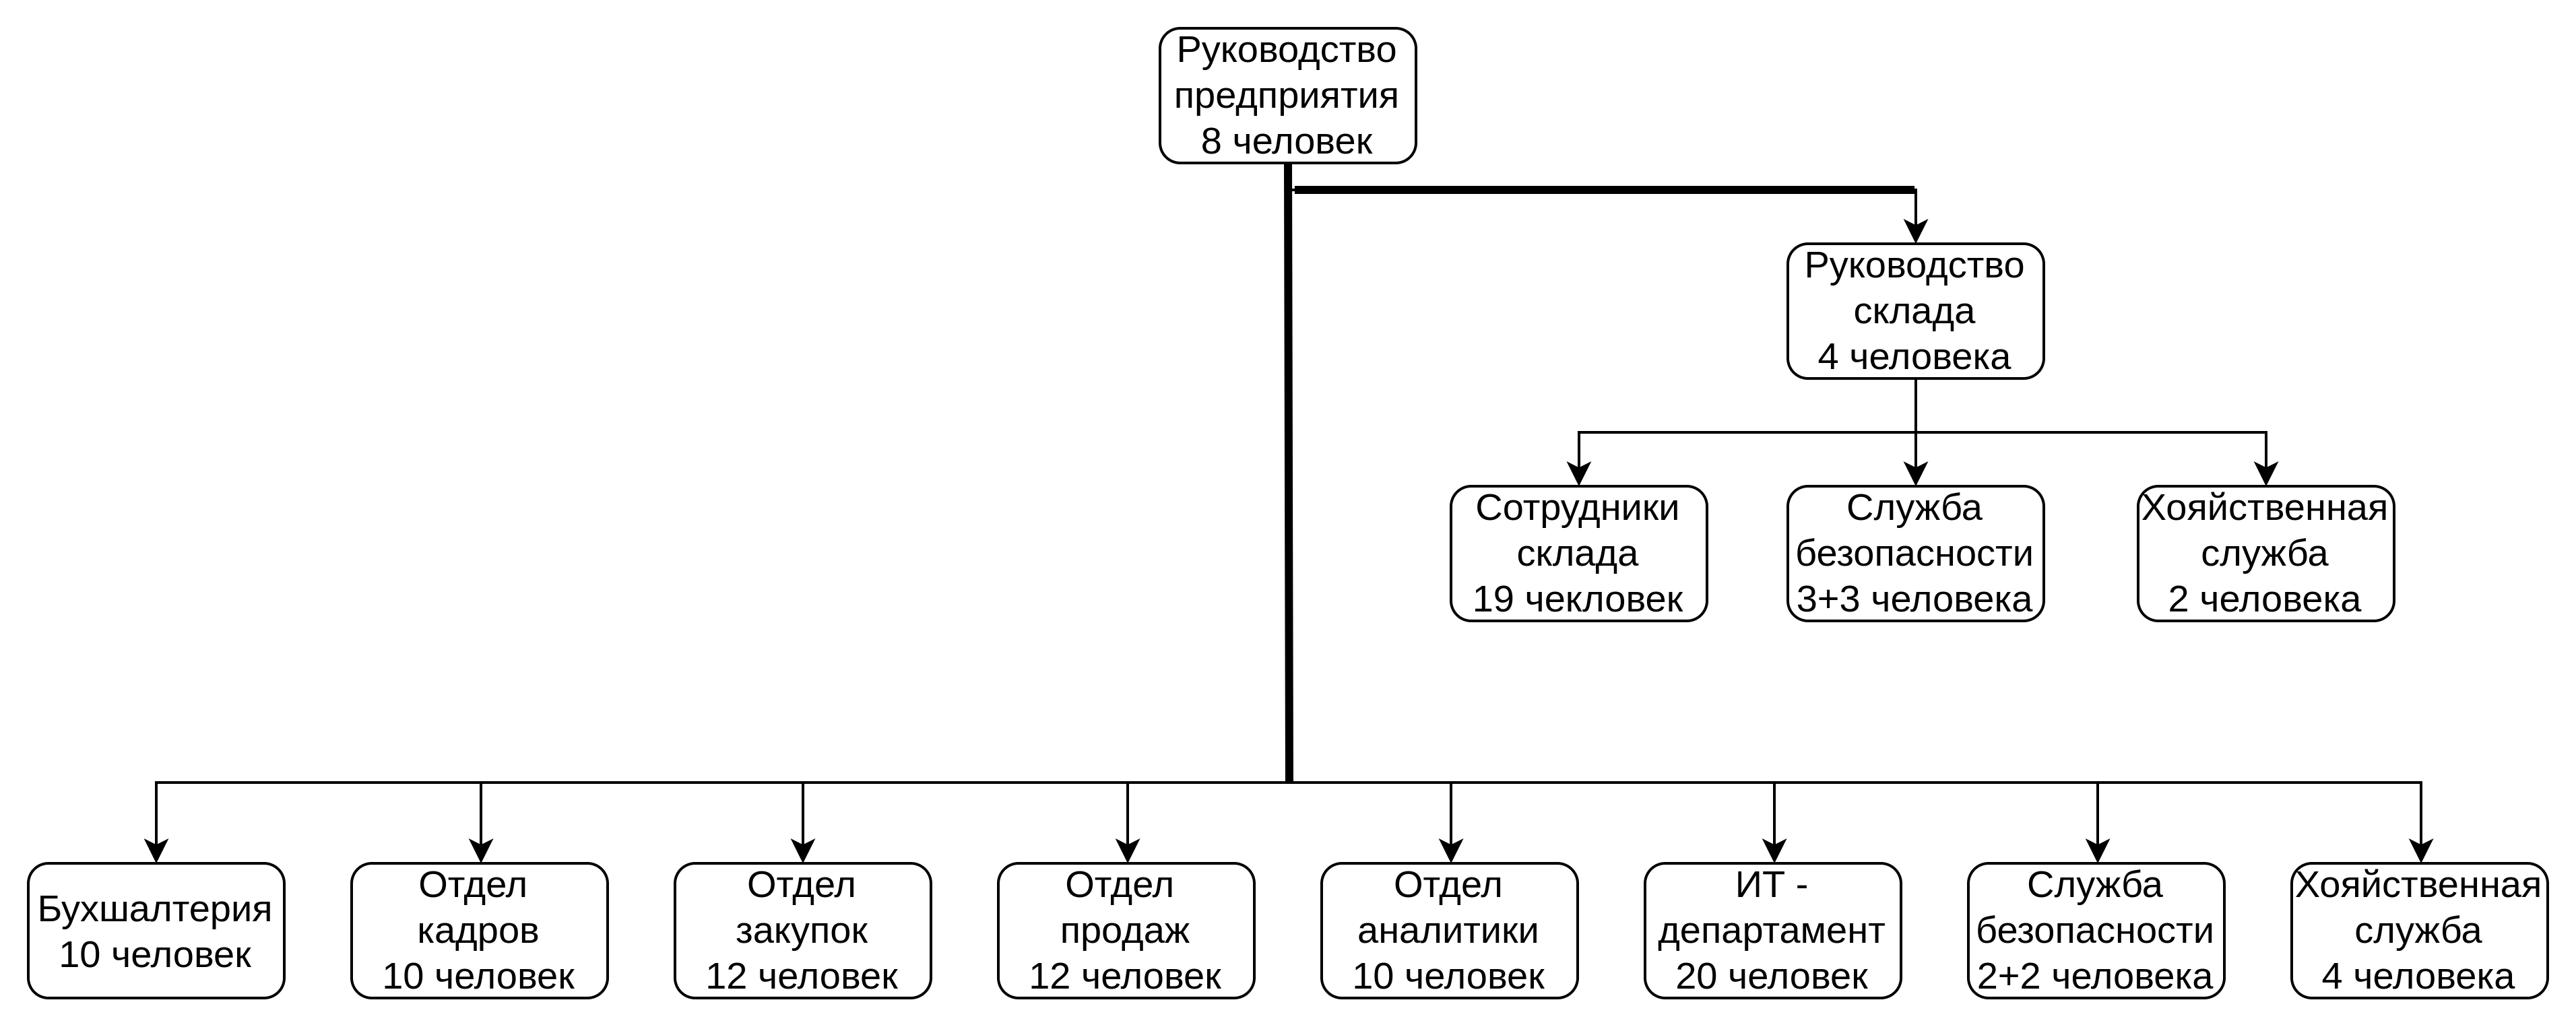
\includegraphics[scale=0.12]{../misc/org_structure_people.png}
\caption{Организационная структура предприятия\label{fig:stucture_people}}
\end{figure}

В основном здании предприятия всего 90 сотрудников, так как а службе охраны и хозяйственной службе в АРМ нуждается не каждый сотрудник и так же с учетом посменной работы, по итоговым расчетом в основном здании достаточно 84 АРМ.

Структура основного здания и склада предприятия по количеству рабочих мест изображена на Рисунках\;\ref{fig:structure_ARM_oz}-\ref{fig:structure_ARM_sk}.


\begin{figure}[H]
\numberwithin{figure}{section}
\centering
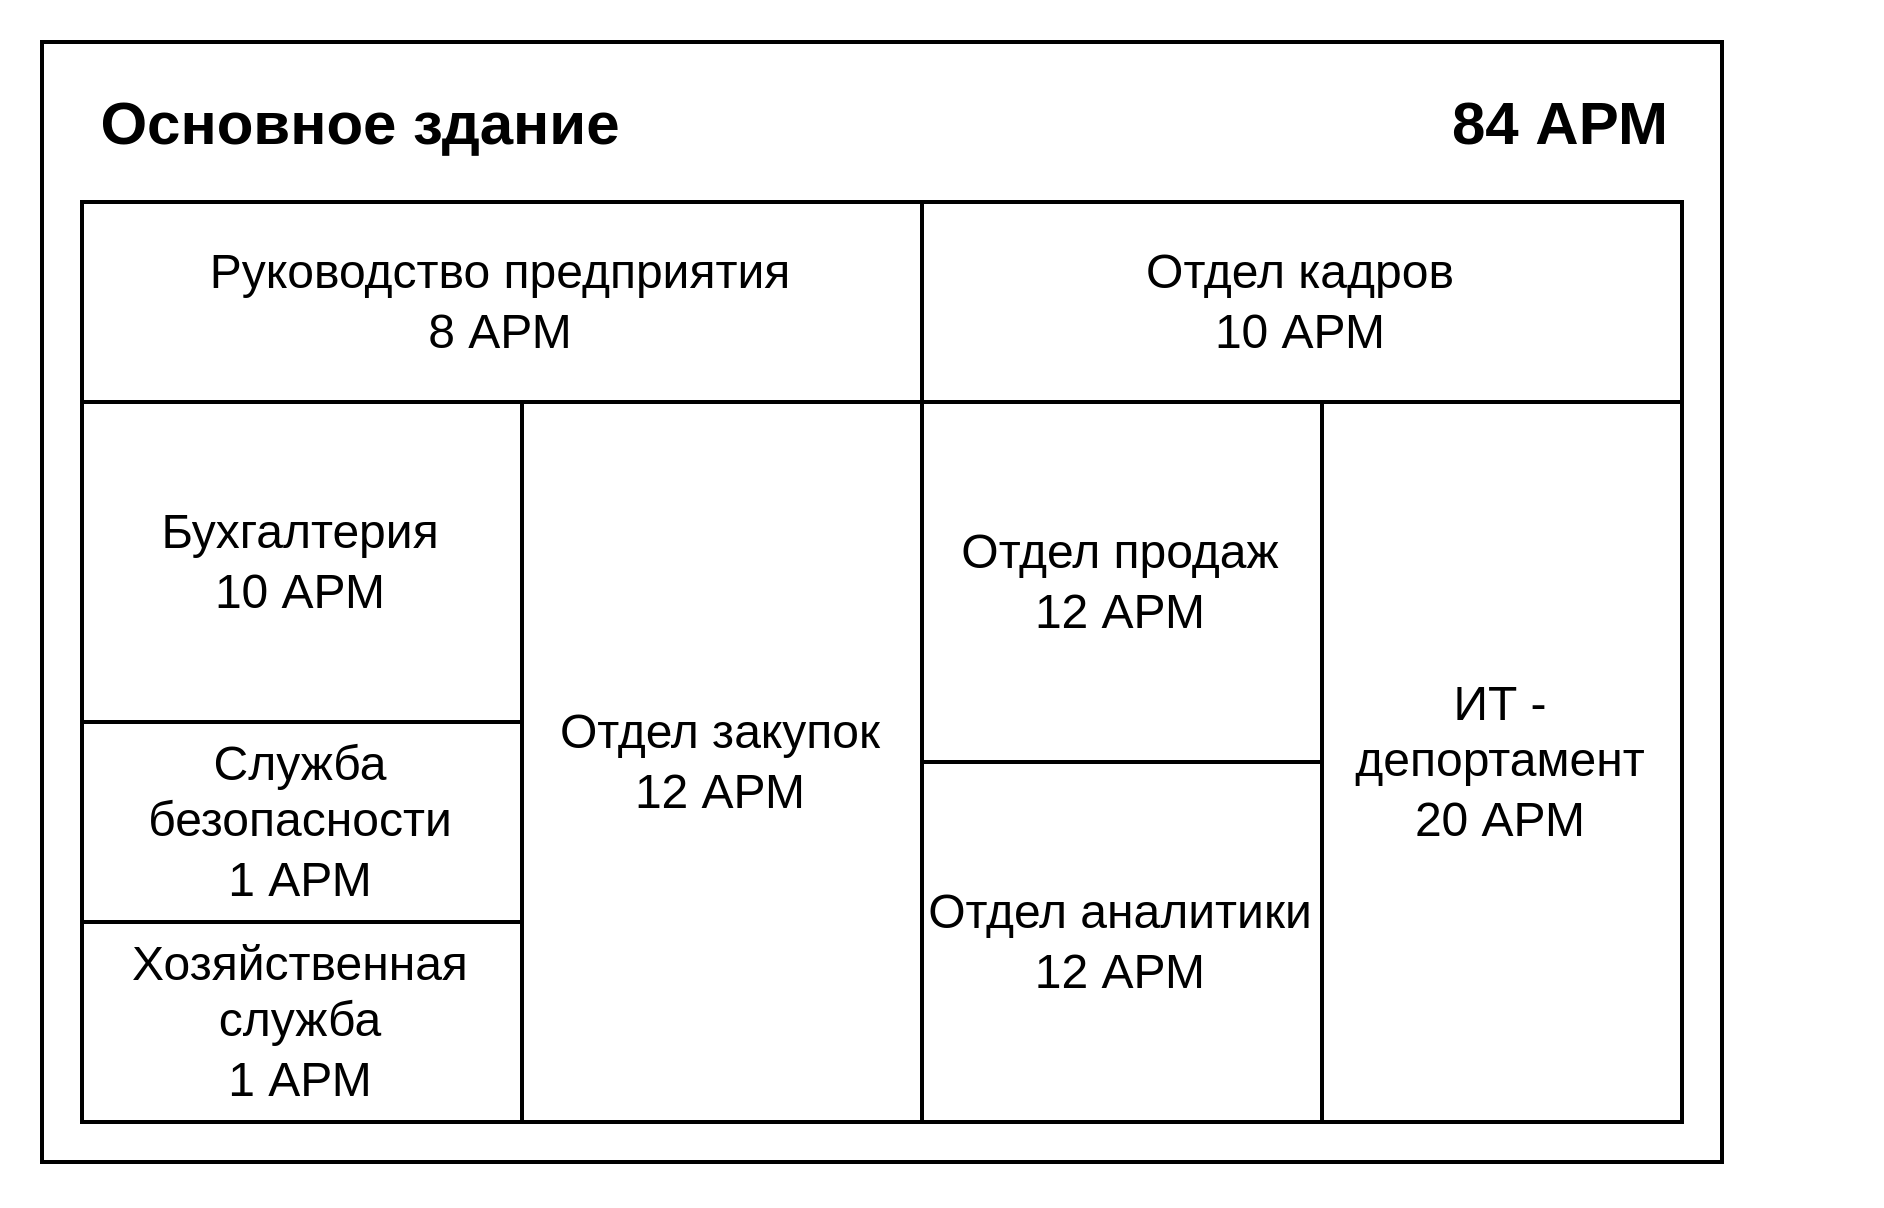
\includegraphics[scale=0.12]{../misc/org_structure_ARM_oz.png}
\caption{Количество рабочих мест в основном здании\label{fig:structure_ARM_oz}}
\end{figure}

На складе всего 30 сотрудников из которых 19 сотрудников это кладовщики, которые не нуждаются в АРМ. Охранной службе достаточно одного АРМ главному по смене сотруднику. Также достаточно одного АРМ для хозяйственной службы для учета выполненной работы.

\begin{figure}[H]
\numberwithin{figure}{section}
\centering
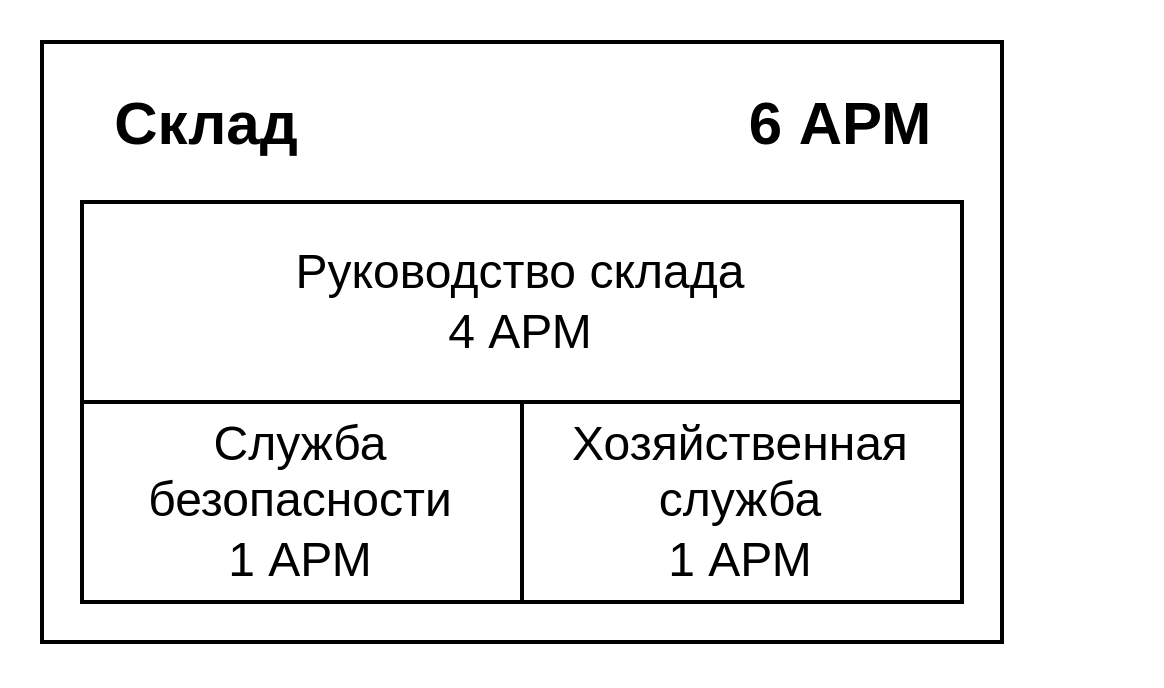
\includegraphics[scale=0.17]{../misc/org_structure_ARM_sk.png}
\caption{Количество рабочих мест на складе\label{fig:structure_ARM_sk}}
\end{figure}

Для всех отделов, основного здания и склада, количество АРМ совпадает с количеством сотрудников, кроме хозяйственной службы, где только заведующий по хозяйству имеет АРМ и службы охраны, которая работает посменно и рабочее место есть только у 1 сотрудника. 





\subsection{Расчет пропускной способности каналов передачи данных}
В данном пункте будет производится расчет пропускной способности каналов передачи данных  с учетом применения трехуровневой архитектуры сети, состоящей из уровня доступа, агрегации я ядра.

Расчеты по количеству портов будут выполняться снизу вверх. На уровне доступа количество портов соответствует количеству терминалов с проводным подключением а так же количеству точек доступа, принтеров, IP-телефонов, IP-камер и других устройств\cite{tcp-mech}.

Скоростные требования к портам для обычных конечных пользователей будет 100 Мбит/с и 1 Гбит/с для конечных пользователей с особыми требованиями, таких как начальство. Так же будет требование 1 Гбит/с к портам для сервера. Количество АРМ и требования к каналу передачи данных для основного здания и склада представлены в Таблицах\;\ref{table:ARM_chanal_oz}-\;\ref{table:ARM_chanal_sk}. Обозначение 100х15 + 1000х5 обозначает, что из общего количества АРМ 15 АРМ требуют канал передачи 100 Мбит/с и 5 АРМ 1000 Мбит/с, так же для склада.


\begin{table}[H]
    \centering
    \numberwithin{table}{section}
    \caption{Требования к каналу передачи данных основного здания\label{table:ARM_chanal_oz}}
    \small
	\begin{tabularx}{\textwidth}{|X|p{2cm}|X|X|}
        \hline
		Название отдела&Количество АРМ&Требования к каналу передачи данных, Мбит/с&Конечная нагрузка на отдел, Мбит/с \\
        \hline
		Руководство предприятия         & 8       		&  	1000				&	8000  \\
		\hline
		Бухгалтерия						& 10         	&  	100					&	1000  \\
        \hline
		Отдел кадров					& 10         	&  	100					&	1000  \\
        \hline
		Отдел закупок					& 12         	&  	100					&	1200  \\
        \hline
		Отдел продаж					& 12         	&  	100					&	1200  \\
        \hline
		Отдел аналитики					& 10         	&  	100					&	1000  \\
        \hline
		ИТ-департамент					& 20         	&  	100х15 + 1000х5		&	6500  \\
        \hline
		Служба безопасности				& 1				& 	100					&	100	  \\
		\hline
		Хозяйственная служба			& 1         	&  	100					&	100  \\
        \hline
		\multicolumn{3}{|X|}{Итого:}											& 20100 \\
		\hline
    \end{tabularx}
\end{table}

\begin{table}[H]
    \centering
    \numberwithin{table}{section}
    \caption{Требования к каналу передачи данных склада\label{table:ARM_chanal_sk}}
    \small
	\begin{tabularx}{\textwidth}{|X|p{2cm}|X|X|}
        \hline
        % \multicolumn{1}{|c|}{Описание подсети} & Количество узлов & сетевой адрес/префикс маски подсети & Первый узловой адрес & Последний узловой адрес \\
		Название отдела&Количество АРМ&Требования к каналу передачи данных, Мбит/с&Конечная нагрузка на отдел, Мбит/с \\
        \hline
		Руководство склада         		& 4       		&  	100х3 + 1000х1		&	1300  \\
		\hline
		Служба безопасности				& 1				& 	100					&	100	  \\
		\hline
		Хозяйственная служба			& 1         	&  	100					&	100  \\
        \hline
		\multicolumn{3}{|X|}{Итого:}											& 1500 \\
		\hline
    \end{tabularx}
\end{table}

Итоговое количество портов полученное на уровне доступа для основного здания 102 с учетом точек доступа, принтеров и ip-телефонов. Было определено, что из них 89 портов FastEthernet и 13 портов GigabitEthernet. Для склада на уровне доступа количество портов составляет 19, с учетом устройств требующих проводное подключение. Было определено, что 18 портов FastEthernet и 1 порт GigabitEthernet. Далее с известным количеством кортов на уровне доступа рассчитывается количество портов на уровне агрегации.

Для расчета количества портов на уровне агрегации исходя из данных уровня доступа необходимо учесть коэффициент перехода. Данный коэффициент рассчитывается из условия требований для узлов, например, для конечных проводных компьютеров данный коэффициент будет равен 40\%, так как узлы не будут постоянно использовать весь канал передачи данных из-за того, что основным сервисом является программное обеспечение 1С: Документооборот, которое не требует особых требований к постоянному широкополосному каналу передачи данных. С другой стороны сервера, подключенные по GigabitEthernet будут тратить более 90\% постоянно по причине развертывания на них различных сервисов, в том числе сервера 1С:Документооборот, к которому будут обращаться конечные пользователи при решении своих задач. В данном расчете для серверов будет взят коэффициент 100\%, а для конечных узлов 40\%.

% Исходя из приведенных данных для уровня доступа и с учетом коэффициента перехода расчет пропускной способности для уровня агрегации основного здания будет иметь следующий вид (Формула\; 2.1).
%
% \begin{equation}
% \numberwithin{equation}{section}
% \begin{split}
% p & = 89 \times 100 \;\frac{\text{Мбит}}{\text{с}} \times 40\% + 13 \times 1000 \;\frac{\text{Мбит}}{\text{с}} \times 40\% \\
% & \quad + 3 \;\text{узлов} \times 1000 \;\frac{\text{Мбит}}{\text{с}}\times 100\% = 11760\;\frac{\text{Мбит}}{\text{с}}
% \end{split}
% \label{eqn:agg_ports}
% \end{equation}


% Требуется минимум 12 портов GigabitEthernet на уровне агрегации для основного здания. На уровне ядра требуется соотношение один к одному для пропускной способности канала (Таблица\;\ref{table:all_ports_oz}).


На основе произведенных выше расчетов и таблиц более полный расчет портов на уровне доступа основного здания и склада будет выглядеть следующим образом (Таблицы\;\ref{table:dostup_ports_oz} -\;\ref{table:dostup_ports_sk}).


\begin{table}[H]
    \centering
    \numberwithin{table}{section}
	\caption{Расчет портов уровня доступа для основного здания\label{table:dostup_ports_oz}}
    \small
	\begin{tabularx}{\textwidth}{|p{2.5cm}|X|X|X|p{2.5cm}|X|}
        \hline
		Название отдела&Количество АРМ&Требования к каналу передачи данных, Мбит/с&Суммарные требования на отдел, Мбит/с & Портов GigabitEthernet & Портов FastEthernet \\
        \hline
		Руководство предприятия         & 8       		&  	1000			&	8000  & 8 & 0	\\
		\hline
		Бухгалтерия						& 10         	&  	100				&	1000  & 0 & 10	\\
        \hline
		Отдел кадров					& 10         	&  	100				&	1000  & 0 & 10 \\
        \hline
		Отдел закупок					& 12         	&  	100				&	1200  & 0 & 12 \\
  %       \hline
		% Отдел продаж					& 12         	&  	100				&	1200  & 0 & 12 \\
  %       \hline
		% Отдел аналитики					& 10         	&  	100				&	1000  & 0 & 10 \\
  %       \hline
		% ИТ-департамент					& 20         	&  	100х15  1000х5	&	6500  & 5 & 15 \\
  %       \hline
		% Служба безопасности				& 1				& 	100				&	100	  & 0 & 1 \\
		% \hline
		% Хозяйственная служба			& 1         	&  	100				&	100   & 0 & 1 \\
  %       \hline
		% Итого							& 84	& \multicolumn{2}{X|}{---}			  &13& 71\\
		% \hline
    \end{tabularx}
\end{table}

\begin{table}[H]
    \centering
    \numberwithin{table}{section}
	\caption{Продолжение таблицы\;\ref{table:dostup_ports_oz}}
    \small
	\begin{tabularx}{\textwidth}{|p{2.5cm}|X|X|X|p{2.5cm}|X|}
        \hline
		Название отдела&Количество АРМ&Требования к каналу передачи данных, Мбит/с&Суммарные требования на отдел, Мбит/с & Портов GigabitEthernet & Портов FastEthernet \\
        \hline
		Отдел продаж					& 12         	&  	100				&	1200  & 0 & 12 \\
        \hline
		Отдел аналитики					& 10         	&  	100				&	1000  & 0 & 10 \\
        \hline
		ИТ-департамент					& 20         	&  	100х15  1000х5	&	6500  & 5 & 15 \\
        \hline
		Служба безопасности				& 1				& 	100				&	100	  & 0 & 1 \\
		\hline
		Хозяйственная служба			& 1         	&  	100				&	100   & 0 & 1 \\
        \hline
		Итого							& 84	& \multicolumn{2}{X|}{---}			  &13& 71\\
		\hline
    \end{tabularx}
\end{table}


\begin{table}[H]
    \centering
    \numberwithin{table}{section}
	\caption{Расчет портов уровня доступа для склада\label{table:dostup_ports_sk}}
    \small
	\begin{tabularx}{\textwidth}{|p{2.5cm}|X|X|X|p{2.5cm}|X|}
        \hline
		Название отдела&Количество АРМ&Требования к каналу передачи данных, Мбит/с&Суммарные требования на отдел, Мбит/с & Портов GigabitEthernet & Портов FastEthernet \\
        \hline
		Руководство склада		        & 4       		&  	3х100 1х1000	&	1300  & 1 & 3	\\
		\hline
		Служба безопасности				& 1				& 	100				&	100	  & 0 & 1 \\
		\hline
		Хозяйственная служба			& 1         	&  	100				&	100   & 0 & 1 \\
        \hline
		Итого							& 6	& \multicolumn{2}{X|}{---}			  & 1 & 4\\
		\hline
    \end{tabularx}
\end{table}

Для расчетов подключения конечных устройств будет взят коэффициент 40\% для перехода на уровень агрегации по причине того, что будут использоваться приложения не сильно чувствительные к задержкам и потерям. Итого расчеты представлены в Таблице\;\ref{table:agr_ports_oz}. Для склада представлены расчеты только для уровня ядра в силу отсутствия уровня агрегации в Таблице\;\ref{table:agr_ports_sk} Следует учитывать, что производится резервирование. Объем трафика при переходе с уровня агрегации на уровень ядра не меняется. Поэтому количество портов на уровне ядра считается по объему трафика на уровне агрегации. Через знак `+' указываются порты, которые являются резервными и будут использованы для предотвращения проблем при выходе из строя основного порта. 

\begin{table}[H]
    \centering
    \numberwithin{table}{section}
	\caption{Расчет портов на уровне агрегации основного здания\label{table:agr_ports_oz}}
    \small
	\begin{tabularx}{\textwidth}{|X|X|X|X|}
        \hline
		Название отдела&Суммарные требования на отдел, Мбит/с & Объем трафика при переходе на уровень агрегации Мбит/с &Количество портов на уровне агрегации, GigabitEthernet \\
        \hline
		Руководство предприятия         &	8000  & 3200 & 4+1	\\
		\hline
		Бухгалтерия						&	1000  & 400 & 1+1	\\
        \hline
		Отдел кадров					&	1000  & 400 & 1+1 \\
        \hline
		Отдел закупок					&	1200  & 480 & 1+1\\
        \hline
		Отдел продаж					&	1200  & 480 & 1+1 \\
        \hline
		Отдел аналитики					&	1000  & 400 & 1+1 \\
        \hline
		ИТ-департамент					&	6500  & 2600 & 3+1 \\
        \hline
		Служба безопасности				&	100	  & 40 & 1+1 \\
		\hline
		Хозяйственная служба			&	100   & 40 & 1+1 \\
        \hline
		Итого							& -		 & 8080 & 24\\
		\hline
    \end{tabularx}
\end{table}

% \begin{table}[H]
%     \centering
%     \numberwithin{table}{section}
% 	\caption{Продолжение таблицы\;\ref{table:agr_ports_oz}}
%     \small
% 	\begin{tabularx}{\textwidth}{|X|X|X|X|}
%         \hline
% 		Название отдела&Суммарные требования на отдел, Мбит/с & Объем трафика при переходе на уровень агрегации Мбит/с &Количество портов на уровне агрегации, GigabitEthernet \\
%         \hline
% 		Руководство предприятия         &	8000  & 3200 & 4+1	\\
% 		\hline
% 		Бухгалтерия						&	1000  & 400 & 1+1	\\
%         \hline
% 		Отдел кадров					&	1000  & 400 & 1+1 \\
%         \hline
% 		Отдел закупок					&	1200  & 480 & 1+1\\
%         \hline
% 		Отдел продаж					&	1200  & 480 & 1+1 \\
%         \hline
% 		Отдел аналитики					&	1000  & 400 & 1+1 \\
%         \hline
% 		ИТ-департамент					&	6500  & 2600 & 3+1 \\
%         \hline
% 		Служба безопасности				&	100	  & 40 & 1+1 \\
% 		\hline
% 		Хозяйственная служба			&	100   & 40 & 1+1 \\
%         \hline
% 		Итого							& -		 & 8080 & 24\\
% 		\hline
%     \end{tabularx}
% \end{table}

Исходя из данных таблицы расчета портов на уровне агрегации, для уровня ядра требуется минимум 9 портов GigabitEthernet в основном здании. Данные по количеству требуемых портов c учетом резервирования представлены в Таблице\;\ref{table:all_ports_oz}.

\begin{table}[H]
    \centering
    \numberwithin{table}{section}
    \caption{Общее количество портов для основного здания\label{table:all_ports_oz}}
    \small
    \begin{tabularx}{\textwidth}{|X|X|X|}
        \hline
		Уровень		& Порты GigabitEthernet	&	порты FastEthernet	\\
        \hline	
		Доступ		& 16       				&  	89					\\
		\hline
		Агрегация	& 24					& 	---					\\
		\hline
		ядро		& 9         			&  	---					\\
        \hline
    \end{tabularx}
\end{table}

\begin{table}[H]
    \centering
    \numberwithin{table}{section}
	\caption{Расчет портов на уровне ядра склада\label{table:agr_ports_sk}}
    \small
	\begin{tabularx}{\textwidth}{|X|X|X|X|}
        \hline
		Название отдела&Суммарные требования на отдел, Мбит/с & Объем трафика на уровне ядра Мбит/с &Количество портов на уровне ядра, GigabitEthernet \\
        \hline
		Руководство склада		         &	1300  & 520 & 1+1	\\
  %       \hline
		% Служба безопасности				&	100	  & 40 & 1+1 \\
		% \hline
		% Хозяйственная служба			&	100   & 40 & 1+1 \\
  %       \hline
		% Итого							& -		 & 600 & 6 \\
		% \hline
    \end{tabularx}
\end{table}

\begin{table}[H]
    \centering
    \numberwithin{table}{section}
	\caption{Продолжение Таблицы\;\ref{table:agr_ports_sk}}
    \small
	\begin{tabularx}{\textwidth}{|X|X|X|X|}
        \hline
		Название отдела&Суммарные требования на отдел, Мбит/с & Объем трафика на уровне ядра Мбит/с &Количество портов на уровне ядра, GigabitEthernet \\
  %       \hline
		% Руководство склада		         &	1300  & 520 & 1+1	\\
        \hline
		Служба безопасности				&	100	  & 40 & 1+1 \\
		\hline
		Хозяйственная служба			&	100   & 40 & 1+1 \\
        \hline
		Итого							& -		 & 600 & 6 \\
		\hline
    \end{tabularx}
\end{table}

Для склада требуется 19 портов на уровне доступа. Исходя из этого для склада можно опустить уровень агрегации и использовать только устройства уровня ядра. По приведенной выше формуле с учетом коэффициента перехода на уровне ядра для склада требуется пропускная способность в 600 Мбит/с. Для склада на уровне ядра требуется 1 порт GigabitEthernet (Таблица\;\ref{table:all_ports_sk}).

\begin{table}[H]
    \centering
    \numberwithin{table}{section}
    \caption{Общее количество портов для склада\label{table:all_ports_sk}}
    \small
    \begin{tabularx}{\textwidth}{|X|X|X|}
        \hline
		Уровень		& Порты GigabitEthernet	&	порты FastEthernet	\\
        \hline	
		Доступ		& 1       				&  	18					\\
		\hline
		Агрегация	& ---					& 	---					\\
		\hline
		ядро		& 6         			&  	---					\\
        \hline
    \end{tabularx}
\end{table}


Расчеты выведенные в таблицах выше являются предварительными для построения первого чернового прототипа и выбора устройств для использования и не учитывают резервирование линков.

\subsection{Прототипирование сети}
На данном шаге будет создан прототип сети с учетом предварительного планирования количества портов, политик резервирования, добавления сервера для развертывания программной инфраструктуры предприятия, трехуровневой архитектуры сети, полученных в предыдущем пункте. При формировании прототипа будет использоваться программное обеспечение draw.io и нотации cisco. 


В Таблицах\;\ref{table:specif_uzlov_sk} -\;\ref{table:specif_uzlov_oz} описаны спецификации промежуточных устройств основного здания. На ней описывается какие порты и устройства используются. Для сети главного здания используются маршрутизатор 4331, так как имеет 3 порта GigabitEthernet, что является необходимым количеством для соединения с коммутаторами L3, коммутаторы L3 3650 24PS с 24 портами GigabitEthernet для соединения с коммутаторами L2 и коммутаторы 2960 с 24 портами FastEthernet для соединения с конечными устройствами. На скале же используются коммутаторы 2950T-24 с 24 портами FastEthernet для соединения с конечными устройствами и маршрутизатор 1240. В перечисленных устройствах модули расширения не будут использоваться, кроме маршрутизатора. Считается, что порты 0/0/1 и 0/0/2 маршрутизатора и порты 1/0/2 коммутаторов SW\_1-2\_L3\_DERDZYAN имеют пропускную способность в 10 GigabitEthernet.  В качестве конечных узлов в основном здании выступают персональные компьютеры. На Рисунках\;\ref{fig:topo_oz} -\;\ref{fig:topo_sk} изображена топология сети основного здания на основе Таблиц\;\ref{table:specif_uzlov_sk} -\;\ref{table:specif_uzlov_oz}. Так как руководству и IT-департаменту требуется довольно большая пропускная способность каналов для них между коммутаторами L3 и коммутатором L2 организованы агрегирование каналов\cite{cisco-etherchannel}, которые позволяют увеличить пропускную способность между участниками сети и способствуют отказоустойчивости.



\begin{table}[H]
    \centering
    \numberwithin{table}{section}
	\caption{Спецификации промежуточных устройств прототипа основного здания\label{table:specif_uzlov_oz}}
    \small
	\begin{tabularx}{\textwidth}{|X|X|X|X|X|}
        \hline
		Модель устройства&Имя устройства& Общее количество портов&Используемые порты (названия, количество) & Свободные порты (названия, количество) \\
        \hline
		Маршрутизатор 4331	&	R\_1\_ DERDZYAN  & 3 порта GigabitEthernet & GigabitEthernet 0/0/0 - 0/0/2 & ---\\
		\hline
		Коммутатор L3 3650 24PS		&	SW\_1\_L3\_ DERDZYAN  & 24 порта GigabitEthernet & GigabitEthernet 1/0/1 - 1/0/15 & GigabitEthernet 1/0/16 - 1/0/24	\\
        \hline
		Коммутатор L3 3650 24PS		&	SW\_2\_L3\_ DERDZYAN  & 24 порта GigabitEthernet & GigabitEthernet 1/0/1 - 1/0/14 & GigabitEthernet 1/0/15 - 1/0/24	\\
        \hline
		Коммутатор L3 3650 24PS		&	SW\_3\_L3\_ DERDZYAN  & 24 порта GigabitEthernet & GigabitEthernet 1/0/1 - 1/0/4 & GigabitEthernet 1/0/5 - 1/0/24	\\
        \hline
		Коммутатор L3 3650 24PS		&	SW\_1\_L2\_ DERDZYAN	& 24 порта GigabitEthernet 						 & GigabitEthernet 1/0/1 - 1/0/13 & GigabitEthernet 1/0/14 - 1/0/24 \\
		% \hline
		% \multirow{5}{*}{Коммутатор 2960}
		% 	&SW\_2\_L2\_ DERDZYAN	& 2 порта GigabitEthernet, 24 порта FastEthernet & FastEthernet 0/1 - 0/10, GigabitEthernet 0/1 - 0/2 & FastEthernet 0/11 - 0/24 \\
		% \cline{2-5}
		% 	&SW\_3\_L2\_ DERDZYAN	& 2 порта GigabitEthernet, 24 порта FastEthernet & FastEthernet 0/1 - 0/10, GigabitEthernet 0/1 - 0/2 & FastEthernet 0/11 - 0/24 \\
		% \cline{2-5}
		% 	&SW\_4\_L2\_ DERDZYAN	& 2 порта GigabitEthernet, 24 порта FastEthernet & FastEthernet 0/1 - 0/12, GigabitEthernet 0/1 - 0/2 & FastEthernet 0/13 - 0/24  \\
		% \cline{2-5}
		% 	&SW\_5\_L2\_ DERDZYAN	& 2 порта GigabitEthernet, 24 порта FastEthernet & FastEthernet 0/1 - 0/12, GigabitEthernet 0/1 - 0/2 & FastEthernet 0/13 - 0/24 \\
		% \cline{2-5}
		% 	&SW\_6\_L2\_ DERDZYAN	& 2 порта GigabitEthernet, 24 порта FastEthernet & FastEthernet 0/1 - 0/10, GigabitEthernet 0/1 - 0/2 & FastEthernet 0/11 - 0/24  \\
		% \hline
		% Коммутатор L3 3650 24PS	&SW\_7\_L2\_ DERDZYAN	& 24 порта GigabitEthernet & GigabitEthernet 1/0/1 - 1/0/24 & --- \\
		% \hline
		% \multirow{3}{*}{Коммутатор 2960}
		% 	&SW\_8\_L2\_ DERDZYAN	& 2 порта GigabitEthernet, 24 порта FastEthernet & FastEthernet 0/1, GigabitEthernet 0/1 - 0/2 & FastEthernet 0/2 - 0/24 \\
		% \cline{2-5}
		% 	&SW\_9\_L2\_ DERDZYAN	& 2 порта GigabitEthernet, 24 порта FastEthernet & FastEthernet 0/1, GigabitEthernet 0/1 - 0/2 & FastEthernet 0/2 - 0/24 \\
		% 	\hline
    \end{tabularx}
\end{table}

\begin{table}[H]
    \centering
    \numberwithin{table}{section}
	\caption{Продолжение Таблицы\;\ref{table:specif_uzlov_oz}}
    \small
	\begin{tabularx}{\textwidth}{|X|X|X|X|X|}
        \hline
		Модель устройства&Имя устройства& Общее количество портов&Используемые порты (названия, количество) & Свободные порты (названия, количество) \\
  %       \hline
		% Маршрутизатор 4331	&	R\_1\_ DERDZYAN  & 3 порта GigabitEthernet & GigabitEthernet 0/0/0 - 0/0/2 & ---\\
		% \hline
		% Коммутатор L3 3650 24PS		&	SW\_1\_L3\_ DERDZYAN  & 24 порта GigabitEthernet & GigabitEthernet 1/0/1 - 1/0/15 & GigabitEthernet 1/0/16 - 1/0/24	\\
  %       \hline
		% Коммутатор L3 3650 24PS		&	SW\_2\_L3\_ DERDZYAN  & 24 порта GigabitEthernet & GigabitEthernet 1/0/1 - 1/0/14 & GigabitEthernet 1/0/15 - 1/0/24	\\
  %       \hline
		% Коммутатор L3 3650 24PS		&	SW\_3\_L3\_ DERDZYAN  & 24 порта GigabitEthernet & GigabitEthernet 1/0/1 - 1/0/4 & GigabitEthernet 1/0/5 - 1/0/24	\\
  %       \hline
		% Коммутатор L3 3650 24PS		&	SW\_1\_L2\_ DERDZYAN	& 24 порта GigabitEthernet 						 & GigabitEthernet 1/0/1 - 1/0/13 & GigabitEthernet 1/0/14 - 1/0/24 \\
		\hline
		\multirow{5}{*}{Коммутатор 2960}
			&SW\_2\_L2\_ DERDZYAN	& 2 порта GigabitEthernet, 24 порта FastEthernet & FastEthernet 0/1 - 0/10, GigabitEthernet 0/1 - 0/2 & FastEthernet 0/11 - 0/24 \\
		\cline{2-5}
			&SW\_3\_L2\_ DERDZYAN	& 2 порта GigabitEthernet, 24 порта FastEthernet & FastEthernet 0/1 - 0/10, GigabitEthernet 0/1 - 0/2 & FastEthernet 0/11 - 0/24 \\
		\cline{2-5}
			&SW\_4\_L2\_ DERDZYAN	& 2 порта GigabitEthernet, 24 порта FastEthernet & FastEthernet 0/1 - 0/12, GigabitEthernet 0/1 - 0/2 & FastEthernet 0/13 - 0/24  \\
		\cline{2-5}
			&SW\_5\_L2\_ DERDZYAN	& 2 порта GigabitEthernet, 24 порта FastEthernet & FastEthernet 0/1 - 0/12, GigabitEthernet 0/1 - 0/2 & FastEthernet 0/13 - 0/24 \\
		\cline{2-5}
			&SW\_6\_L2\_ DERDZYAN	& 2 порта GigabitEthernet, 24 порта FastEthernet & FastEthernet 0/1 - 0/10, GigabitEthernet 0/1 - 0/2 & FastEthernet 0/11 - 0/24  \\
		\hline
		Коммутатор L3 3650 24PS	&SW\_7\_L2\_ DERDZYAN	& 24 порта GigabitEthernet & GigabitEthernet 1/0/1 - 1/0/24 & --- \\
		\hline
		\multirow{3}{*}{Коммутатор 2960}
			&SW\_8\_L2\_ DERDZYAN	& 2 порта GigabitEthernet, 24 порта FastEthernet & FastEthernet 0/1, GigabitEthernet 0/1 - 0/2 & FastEthernet 0/2 - 0/24 \\
		\cline{2-5}
			&SW\_9\_L2\_ DERDZYAN	& 2 порта GigabitEthernet, 24 порта FastEthernet & FastEthernet 0/1, GigabitEthernet 0/1 - 0/2 & FastEthernet 0/2 - 0/24 \\
			\hline
    \end{tabularx}
\end{table}

\begin{table}[H]
    \centering
    \numberwithin{table}{section}
	\caption{Спецификации промежуточных устройств прототипа склада\label{table:specif_uzlov_sk}}
    \small
	\begin{tabularx}{\textwidth}{|X|X|X|X|X|}
        \hline
		Модель устройства&Имя устройства& Общее количество портов&Используемые порты (названия, количество) & Свободные порты (названия, количество) \\
        \hline
		Маршрутизатор 1941	&	R\_1\_ DERDZYAN  & 2 порта GigabitEthernet & GigabitEthernet 0/0/1  &	GigabitEthernet 0/0/2	\\
		\hline
		Коммутатор 2950T-24		&	SW\_1\_L3\_ DERDZYAN  & 24 порта FastEthernet, 2 порта GigabitEthernet & GigabitEthernet 1/0/1 - 1/0/2, FastEthernet 1/0/1 - 1/0/5 & FastEthernet 0/6 - 0/24	\\
		\hline
    \end{tabularx}
\end{table}

\begin{figure}[H]
\numberwithin{figure}{section}
\centering
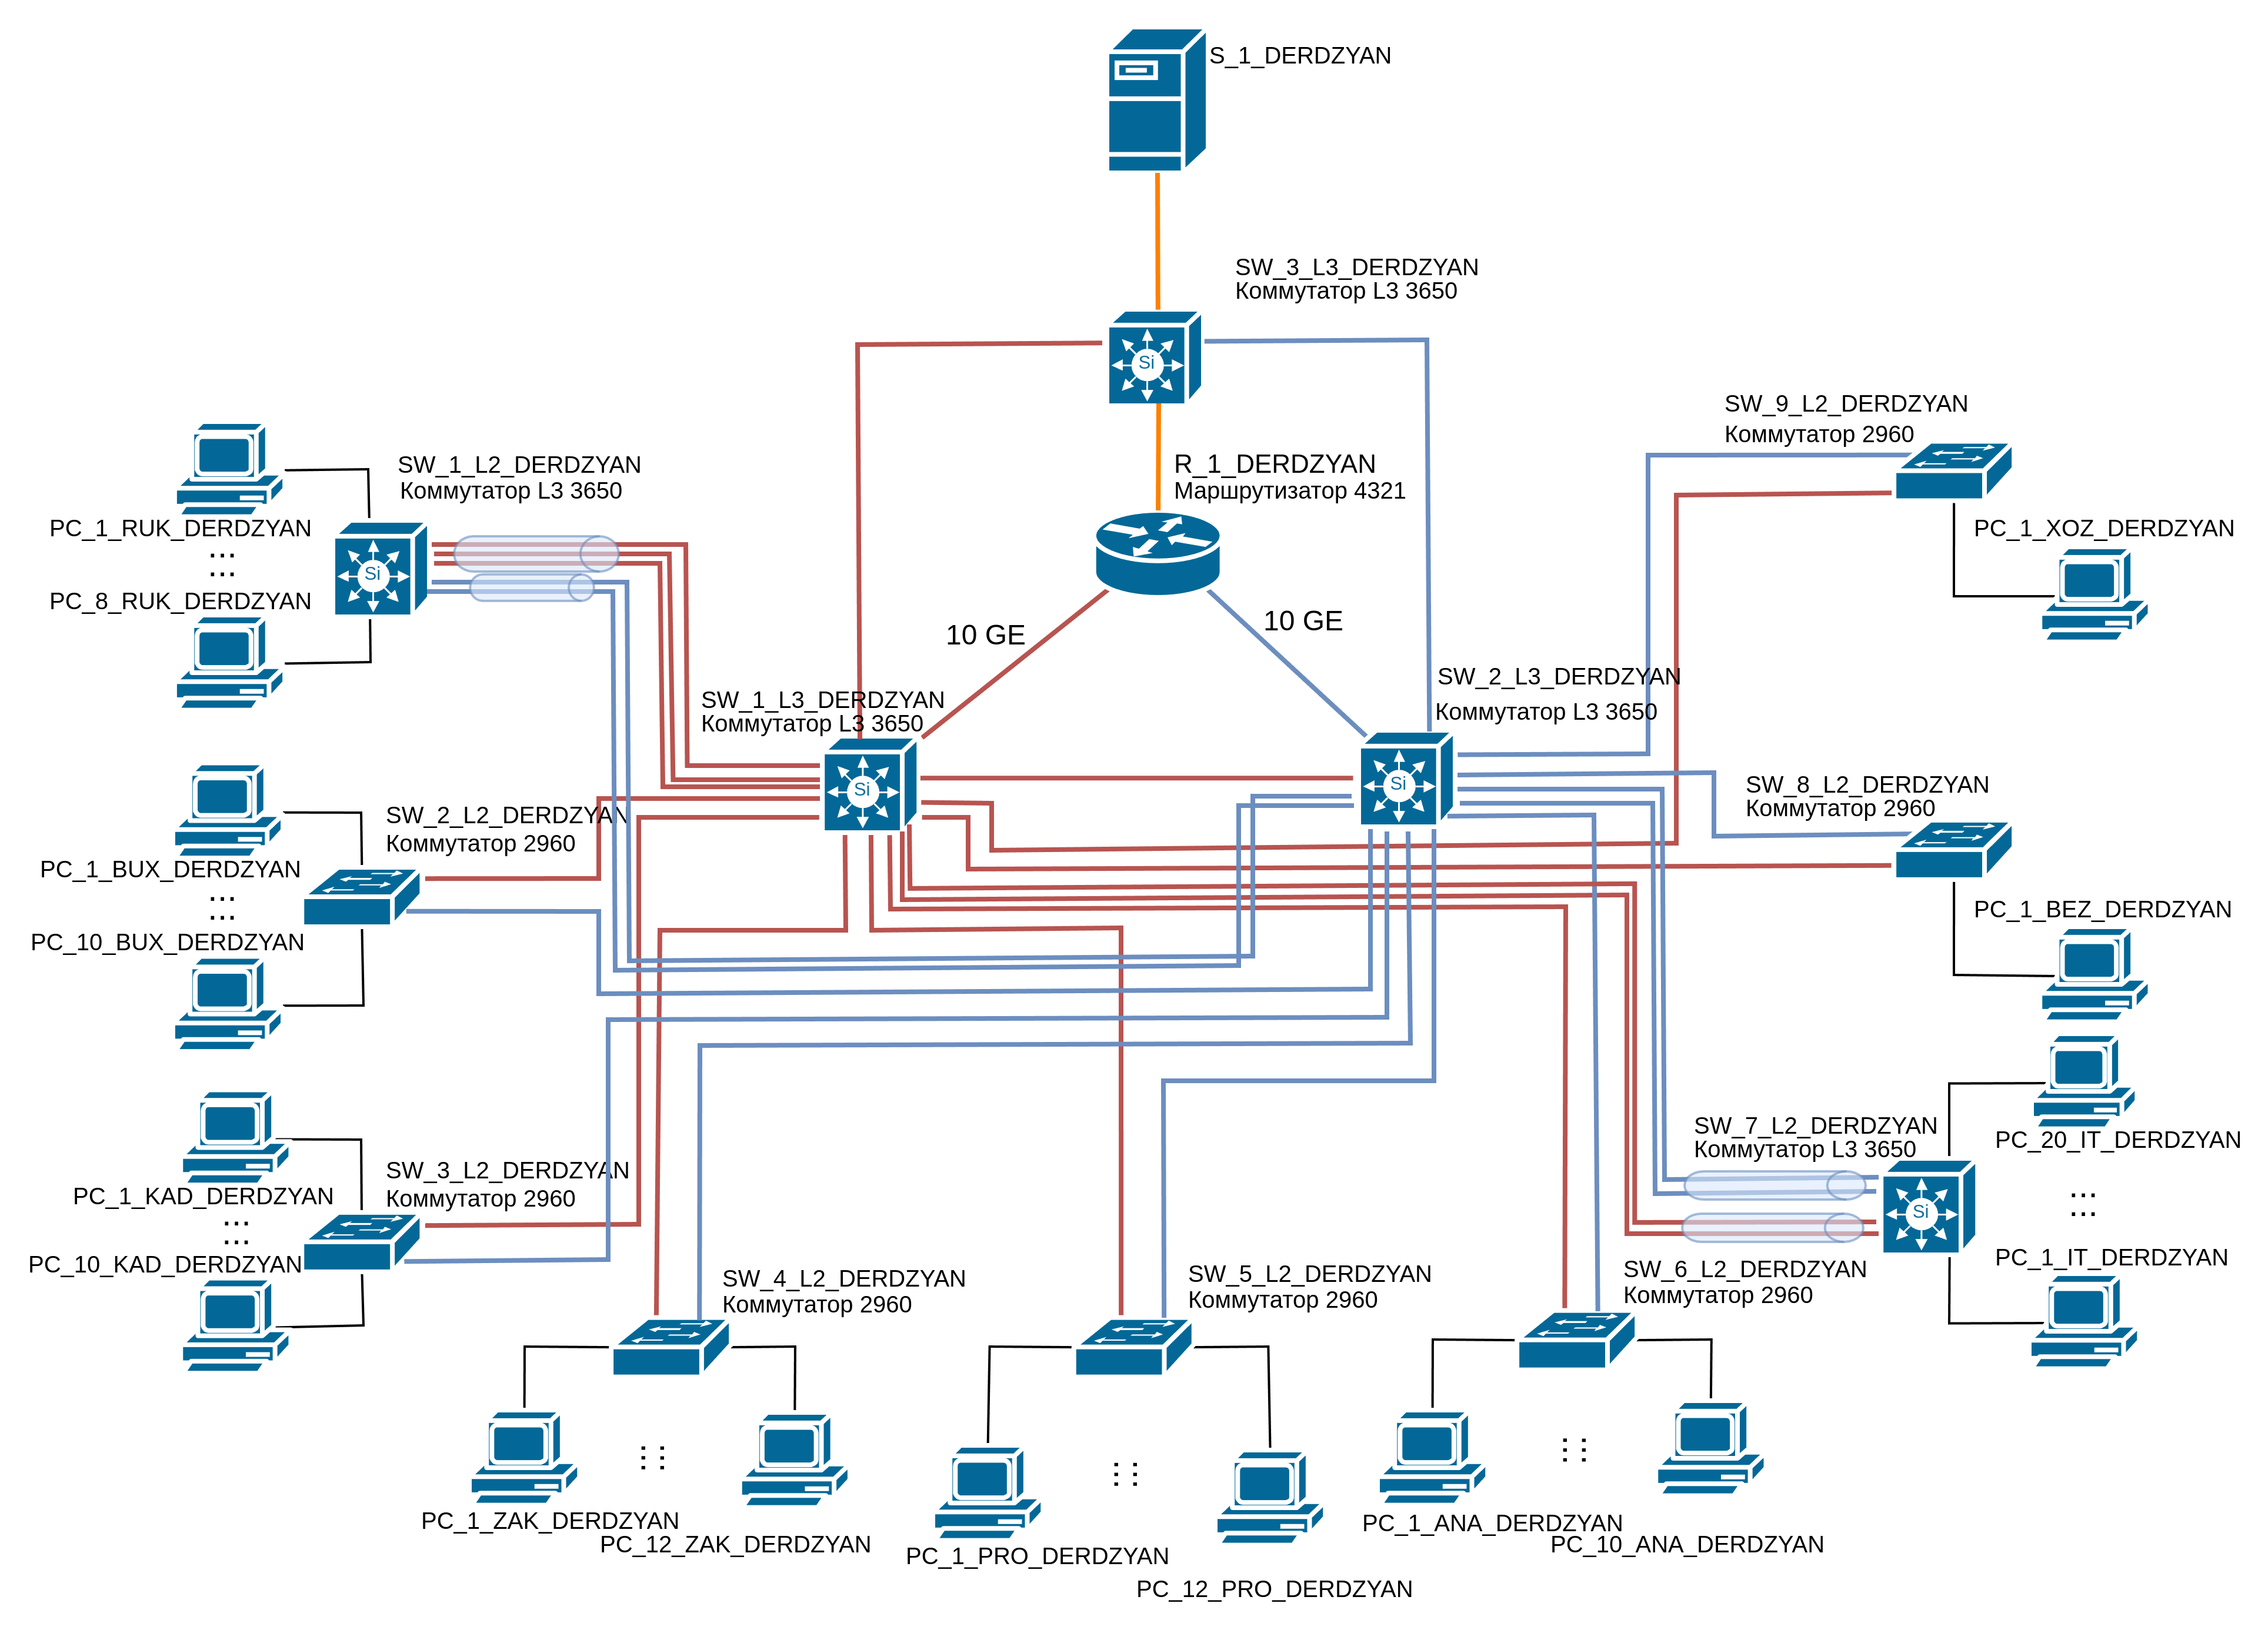
\includegraphics[scale=0.12]{../misc/topo_oz.png}
\caption{Проектирование топологии сети основного здания\label{fig:topo_oz}}
\end{figure}

\begin{figure}[H]
\numberwithin{figure}{section}
\centering
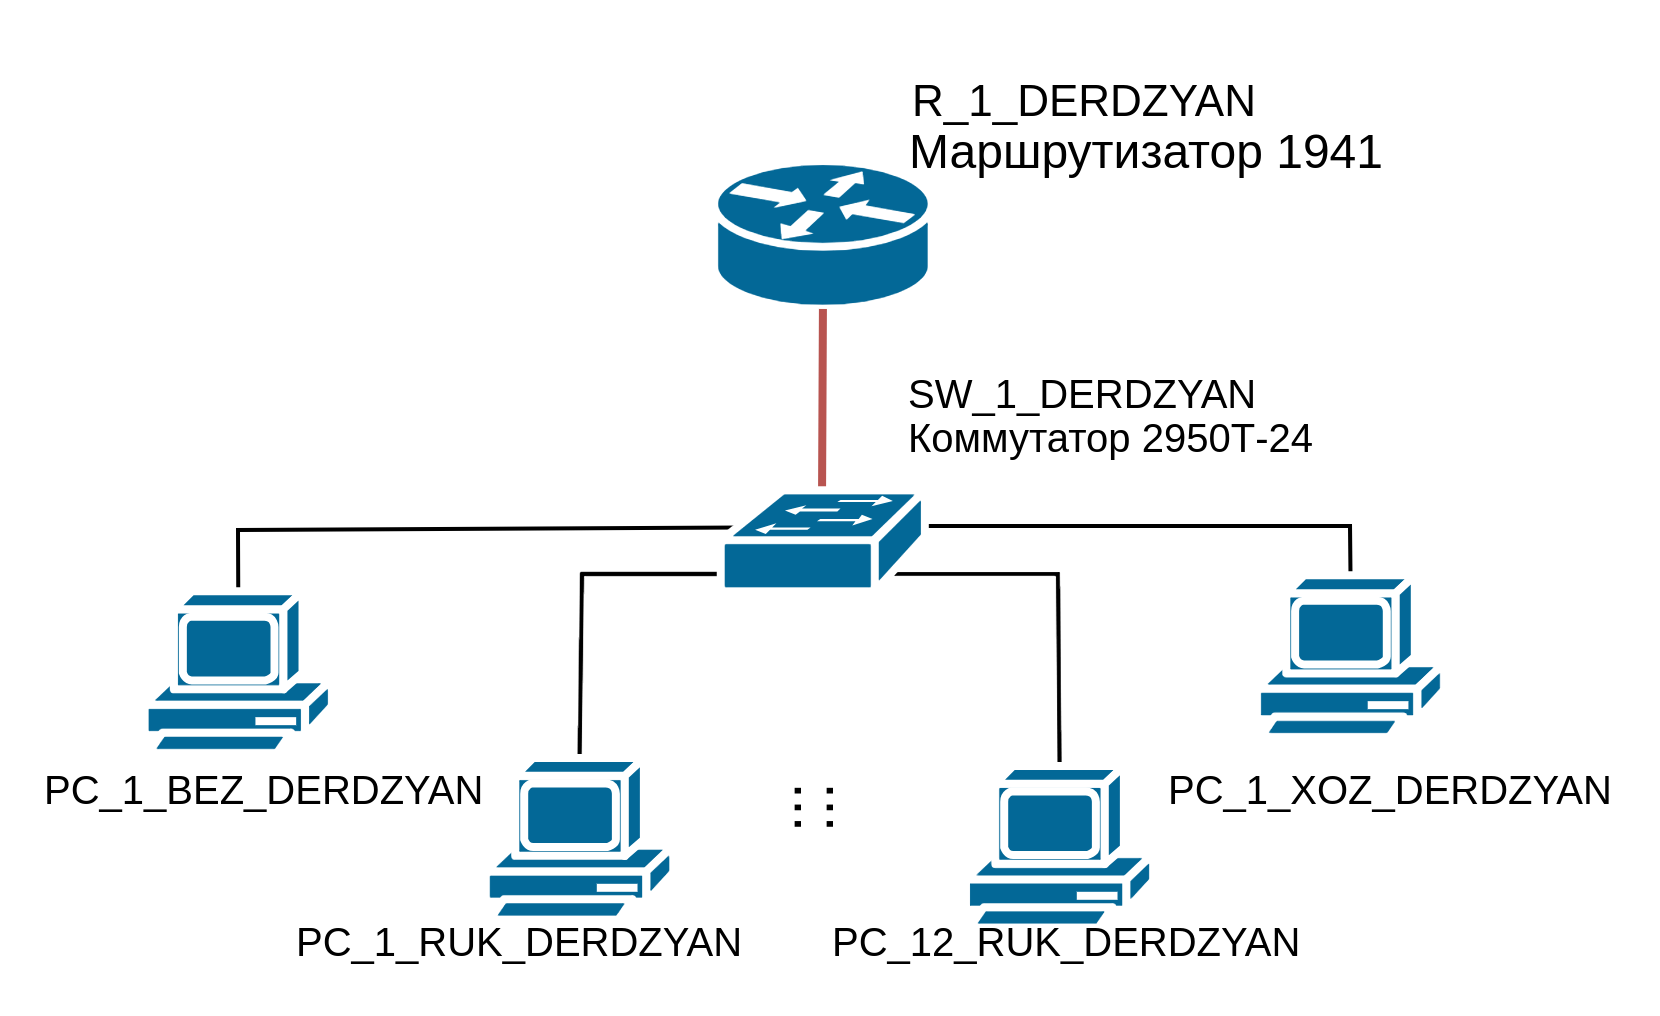
\includegraphics[scale=0.20]{../misc/topo_sk.png}
\caption{Проектирование топологии сети склада\label{fig:topo_sk}}
\end{figure}

В Таблицах\;\ref{table:plan_ports_oz} -\;\ref{table:plan_ports_sk} представлен план подключения промежуточных устройств в основном здании и складе по портам.

\begin{table}[H]
    \centering
    \numberwithin{table}{section}
	\caption{План подключения оборудования по портам для основного здания\label{table:plan_ports_oz}}
    \small
	\begin{tabularx}{\textwidth}{|X|X|X|}
        \hline
		Название устройства& Порт&Описание подключения \\
        \hline
		\multirow{1}{*}{R\_1\_ DERDZYAN} & GigabitEthernet 0/0/1 - 0/0/3 & SW\_1-3\_L3\_DERDZYAN \\
		\hline
		\multirow{3}{*}{SW\_1\_L3\_DERDZYAN} & GigabitEthernet 1/0/2 &  R\_1\_ DERDZYAN \\
		\cline{2-3}
			& GigabitEthernet 1/0/1, 1/0/3 & SW\_2-3\_L3\_DERDZYAN \\
		\cline{2-3}
			& GigabitEthernet 1/0/4 - 1/0/15 & SW\_1-9\_L2\_DERDZYAN \\
		\hline
		\multirow{3}{*}{SW\_2\_L3\_DERDZYAN} & GigabitEthernet 1/0/2 &  R\_1\_ DERDZYAN \\
		\cline{2-3}
			& GigabitEthernet 1/0/1, 1/0/3 & SW\_1, 3\_L3\_DERDZYAN \\
		\cline{2-3}
			& GigabitEthernet 1/0/4 - 1/0/14 & SW\_1-9\_L2\_DERDZYAN \\
		\hline
		\multirow{3}{*}{SW\_3\_L3\_DERDZYAN} & GigabitEthernet 1/0/3 &  R\_1\_ DERDZYAN \\
		\cline{2-3}
			& GigabitEthernet 1/0/2, 1/0/4 & SW\_1-2\_L3\_DERDZYAN \\
		\cline{2-3}
			& GigabitEthernet 1/0/1 & S\_1\_DERDZYAN \\
		\hline
		\multirow{2}{*}{SW\_1\_L2\_DERDZYAN} & GigabitEthernet 1/0/1 - 1/0/3 & SW\_1\_L3\_DERDZYAN  \\
		\cline{2-3}
			& GigabitEthernet 1/0/4 - 1/0/6 & SW\_2\_L3\_DERDZYAN  \\
		\cline{2-3}
			& GigabitEthernet 1/0/7 - 1/0/15 & PC\_1-8\_RUK\_DERDZYAN \\
		\hline
		\multirow{2}{*}{SW\_2\_L2\_DERDZYAN} & GigabitEthernet 0/1 - 0/2 & SW\_1-2\_L3\_DERDZYAN  \\
		\cline{2-3}
			& FastEthernet 0/1 - 0/10 & PC\_1-10\_BUX\_DERDZYAN \\
		\hline
		\multirow{2}{*}{SW\_3\_L2\_DERDZYAN} & GigabitEthernet 0/1 - 0/2 & SW\_1-2\_L3\_DERDZYAN  \\
		\cline{2-3}
			& FastEthernet 0/1 - 0/10 & PC\_1-10\_KAD\_DERDZYAN \\
		\hline
		\multirow{2}{*}{SW\_4\_L2\_DERDZYAN} & GigabitEthernet 0/1 - 0/2 & SW\_1-2\_L3\_DERDZYAN  \\
		\cline{2-3}
			& FastEthernet 0/1 - 0/12 & PC\_1-12\_ZAK\_DERDZYAN \\
		\hline
		\multirow{2}{*}{SW\_5\_L2\_DERDZYAN} & GigabitEthernet 0/1 - 0/2 & SW\_1-2\_L3\_DERDZYAN  \\
		\cline{2-3}
			& FastEthernet 0/1 - 0/10 & PC\_1-10\_PRO\_DERDZYAN \\
		% \hline
		% \multirow{2}{*}{SW\_6\_L2\_DERDZYAN} & GigabitEthernet 0/1 - 0/2 & SW\_1-2\_L3\_DERDZYAN  \\
		% \cline{2-3}
		% 	& FastEthernet 0/1 - 0/10 & PC\_1-10\_ANA\_DERDZYAN \\
		% \hline
		% \multirow{2}{*}{SW\_7\_L2\_DERDZYAN} & GigabitEthernet 1/0/1 - 1/0/4 & SW\_1-2\_L3\_DERDZYAN  \\
		% \cline{2-3}
		% 	& GigabitEthernet 1/0/5 - 1/0/24 & PC\_1-20\_IT\_DERDZYAN \\
		% \hline
		% \multirow{2}{*}{SW\_8\_L2\_DERDZYAN} & GigabitEthernet 0/1 - 0/2 & SW\_1-2\_L3\_DERDZYAN  \\
		% \cline{2-3}
		% 	& FastEthernet 0/1 & PC\_1\_BEZ\_DERDZYAN \\
		% \hline
		% \multirow{2}{*}{SW\_9\_L2\_DERDZYAN} & GigabitEthernet 0/1 - 0/2 & SW\_1-2\_L3\_DERDZYAN  \\
		% \cline{2-3}
		% 	& FastEthernet 0/1 & PC\_1\_XOZ\_DERDZYAN \\
		% \hline
    \end{tabularx}
\end{table}

\begin{table}[H]
    \centering
    \numberwithin{table}{section}
	\caption{Продолжение Таблицы\;\ref{table:plan_ports_oz}}
    \small
	\begin{tabularx}{\textwidth}{|X|X|X|}
        \hline
		Название устройства& Порт&Описание подключения \\
        \hline
		% \multirow{1}{*}{R\_1\_ DERDZYAN} & GigabitEthernet 0/0/1 - 0/0/3 & SW\_1-3\_L3\_DERDZYAN \\
		% \hline
		% \multirow{3}{*}{SW\_1\_L3\_DERDZYAN} & GigabitEthernet 1/0/2 &  R\_1\_ DERDZYAN \\
		% \cline{2-3}
		% 	& GigabitEthernet 1/0/1, 1/0/3 & SW\_2-3\_L3\_DERDZYAN \\
		% \cline{2-3}
		% 	& GigabitEthernet 1/0/4 - 1/0/15 & SW\_1-9\_L2\_DERDZYAN \\
		% \hline
		% \multirow{3}{*}{SW\_2\_L3\_DERDZYAN} & GigabitEthernet 1/0/2 &  R\_1\_ DERDZYAN \\
		% \cline{2-3}
		% 	& GigabitEthernet 1/0/1, 1/0/3 & SW\_1, 3\_L3\_DERDZYAN \\
		% \cline{2-3}
		% 	& GigabitEthernet 1/0/4 - 1/0/14 & SW\_1-9\_L2\_DERDZYAN \\
		% \hline
		% \multirow{3}{*}{SW\_3\_L3\_DERDZYAN} & GigabitEthernet 1/0/3 &  R\_1\_ DERDZYAN \\
		% \cline{2-3}
		% 	& GigabitEthernet 1/0/2, 1/0/4 & SW\_1-2\_L3\_DERDZYAN \\
		% \cline{2-3}
		% 	& GigabitEthernet 1/0/1 & S\_1\_DERDZYAN \\
		% \hline
		% \multirow{2}{*}{SW\_1\_L2\_DERDZYAN} & GigabitEthernet 1/0/1 - 1/0/3 & SW\_1\_L3\_DERDZYAN  \\
		% \cline{2-3}
		% 	& GigabitEthernet 1/0/4 - 1/0/6 & SW\_2\_L3\_DERDZYAN  \\
		% \cline{2-3}
		% 	& GigabitEthernet 1/0/7 - 1/0/15 & PC\_1-8\_RUK\_DERDZYAN \\
		% \multirow{2}{*}{SW\_2\_L2\_DERDZYAN} & GigabitEthernet 0/1 - 0/2 & SW\_1-2\_L3\_DERDZYAN  \\
		% \cline{2-3}
		% 	& FastEthernet 0/1 - 0/10 & PC\_1-10\_BUX\_DERDZYAN \\
		% \hline
		% \multirow{2}{*}{SW\_3\_L2\_DERDZYAN} & GigabitEthernet 0/1 - 0/2 & SW\_1-2\_L3\_DERDZYAN  \\
		% \cline{2-3}
		% 	& FastEthernet 0/1 - 0/10 & PC\_1-10\_KAD\_DERDZYAN \\
		% \hline
		% \multirow{2}{*}{SW\_4\_L2\_DERDZYAN} & GigabitEthernet 0/1 - 0/2 & SW\_1-2\_L3\_DERDZYAN  \\
		% \cline{2-3}
		% 	& FastEthernet 0/1 - 0/12 & PC\_1-12\_ZAK\_DERDZYAN \\
		% \hline
		% \multirow{2}{*}{SW\_5\_L2\_DERDZYAN} & GigabitEthernet 0/1 - 0/2 & SW\_1-2\_L3\_DERDZYAN  \\
		% \cline{2-3}
		% 	& FastEthernet 0/1 - 0/10 & PC\_1-10\_PRO\_DERDZYAN \\
		% \hline
		\multirow{2}{*}{SW\_6\_L2\_DERDZYAN} & GigabitEthernet 0/1 - 0/2 & SW\_1-2\_L3\_DERDZYAN  \\
		\cline{2-3}
			& FastEthernet 0/1 - 0/10 & PC\_1-10\_ANA\_DERDZYAN \\
		\hline
		\multirow{2}{*}{SW\_7\_L2\_DERDZYAN} & GigabitEthernet 1/0/1 - 1/0/4 & SW\_1-2\_L3\_DERDZYAN  \\
		\cline{2-3}
			& GigabitEthernet 1/0/5 - 1/0/24 & PC\_1-20\_IT\_DERDZYAN \\
		\hline
		\multirow{2}{*}{SW\_8\_L2\_DERDZYAN} & GigabitEthernet 0/1 - 0/2 & SW\_1-2\_L3\_DERDZYAN  \\
		\cline{2-3}
			& FastEthernet 0/1 & PC\_1\_BEZ\_DERDZYAN \\
		\hline
		\multirow{2}{*}{SW\_9\_L2\_DERDZYAN} & GigabitEthernet 0/1 - 0/2 & SW\_1-2\_L3\_DERDZYAN  \\
		\cline{2-3}
			& FastEthernet 0/1 & PC\_1\_XOZ\_DERDZYAN \\
		\hline
    \end{tabularx}
\end{table}

\begin{table}[H]
    \centering
    \numberwithin{table}{section}
	\caption{План подключения оборудования по портам для склада\label{table:plan_ports_sk}}
    \small
	\begin{tabularx}{\textwidth}{|X|X|X|}
        \hline
		Название устройства& Порт&Описание подключения \\
        \hline
		R\_1\_ DERDZYAN & GigabitEthernet 0/0/1 & SW\_1\_DERDZYAN \\
		\hline
		\multirow{4}{*}{SW\_1\_DERDZYAN} & FastEthernet 1/0/1 &  PC\_1\_BEZ\_DERDZYAN \\
		\cline{2-3}
			& FastEthernet 1/0/2 & PC\_1\_XOZ\_DERDZYAN \\
		\cline{2-3}
			& GigabitEthernet 1/0/3  & PC\_1\_RUK\_DERDZYAN \\
		\cline{2-3}
			& FastEthernet 1/0/4 - 1/0/6 & PC\_2-4\_RUK\_DERDZYAN \\
		\hline
    \end{tabularx}
\end{table}

\subsection{Планирование сети уровня 2}

Данный этап планирования предназначен для уровня 2 --- проектирование виртуальных локальных сетей (VLAN).Виртуальные локальные сети разделены на сервисные VLAN, управляющие VLAN и взаимосвязанные VLAN. VLAN позволяет создавать виртуальные группы устройств, которые могут взаимодействовать друг с другом, независимо от их физического расположения в сети.

Использование технологии VLAN\cite{query-theory} позволяет предприятиям более гибко и эффективно управлять своей сетью, сокращать затраты на физические маршрутизаторы и обеспечивать лучшую изоляцию и безопасность для различных частей сети.

При проектировании сервисной локальной сети учитывается, что она предназначена для обеспечения доступности сервисов для пользователей. Приведенные VLAN назначены на основе логических областей и по типу услуг разных отделов предприятия.

Управляющий VLAN используется для удаленного доступа к устройствам и управления ими. Коммутаторы уровня 2 используют адреса виртуального интерфейса VLAN в качестве адресов управления. Все коммутаторы одной сети уровня 2 используют одну и ту же управляющую VLAN, а их IP-адреса управления находятся в одном сегменте сети. Взаимосвязанные VLAN нужны для соединения устройств при переходе с уровня агрегации на уровень ядра.

\begin{enumerate}
        \item Управляющая VLAN зарезервирована для устройств уровня 2;
        \item Сеть VLAN подразделяется на гостевую VLAN и так же для каждого отдела предприятия отдельный VLAN;
        \item Коммутаторы уровня 3 подключены к маршрутизаторам через интерфейс VLANIF используя взаимосвязанный VLAN.
\end{enumerate}

Результат планирования VLAN представлен в Таблице\;\ref{table:VLANS_oz}.

\begin{table}[H]
    \centering
    \numberwithin{table}{section}
	\caption{Результат планирования VLAN для основного здания\label{table:VLANS_oz}}
    \small
	\begin{tabularx}{\textwidth}{|X|X|X|}
        \hline
		Идентификатор VLAN (VID)& Имя VLAN & Описание \\ \hline
		2		&	Management\_L2	&	Управляющая VLAN устройств уровня 2 \\ \hline
		3		& Interconnected\_1	&	Взаимосвязанная VLAN между SW\_1\_L3\_ DERDZYAN и R\_1\_ DERDZYAN \\ \hline
		4		& Interconnected\_2	&	Взаимосвязанная VLAN между SW\_2\_L3\_ DERDZYAN и R\_1\_ DERDZYAN \\ \hline
		5		& Interconnected\_3	&	Взаимосвязанная VLAN между SW\_3\_L3\_ DERDZYAN и R\_1\_ DERDZYAN \\ \hline
        101     & Admin        		& Руководство предприятия       \\ \hline
        102     & Accaunting    	& Бухгалтерия                   \\ \hline
        103     & HR            	& Отдел кадров                  \\ \hline
        104     & Purchasing    	& Отдел закупок                 \\ \hline
        105     & Sales        		& Отдел продаж                  \\ \hline
        106     & Analytics     	& Отдел аналитики               \\ \hline
        107     & IT            	& ИТ --- департамент            \\ 
  %       108     & Security      	& Служба безопасности           \\ \hline
		% 109     & Service       	& Хозяйственная безопасности    \\ \hline
		% 111		& Server			& VLAN для сервера				\\ \hline
    \end{tabularx}
\end{table}

\begin{table}[H]
    \centering
    \numberwithin{table}{section}
	\caption{Продолжение Таблицы\;\ref{table:VLANS_oz}}
    \small
	\begin{tabularx}{\textwidth}{|X|X|X|}
        \hline
		Идентификатор VLAN (VID)& Имя VLAN & Описание \\ \hline
		% 2		&	Management\_L2	&	Управляющая VLAN устройств уровня 2 \\ \hline
		% 3		& Interconnected\_1	&	Взаимосвязанная VLAN между SW\_1\_L3\_ DERDZYAN и R\_1\_ DERDZYAN \\ \hline
		% 4		& Interconnected\_2	&	Взаимосвязанная VLAN между SW\_2\_L3\_ DERDZYAN и R\_1\_ DERDZYAN \\ \hline
		% 5		& Interconnected\_3	&	Взаимосвязанная VLAN между SW\_3\_L3\_ DERDZYAN и R\_1\_ DERDZYAN \\ \hline
  %       101     & Admin        		& Руководство предприятия       \\ \hline
  %       102     & Accaunting    	& Бухгалтерия                   \\ \hline
  %       103     & HR            	& Отдел кадров                  \\ \hline
  %       104     & Purchasing    	& Отдел закупок                 \\ \hline
  %       105     & Sales        		& Отдел продаж                  \\ \hline
  %       106     & Analytics     	& Отдел аналитики               \\ \hline
  %       107     & IT            	& ИТ --- департамент            \\ \hline
        108     & Security      	& Служба безопасности           \\ \hline
		109     & Service       	& Хозяйственная безопасности    \\ \hline
		111		& Server			& VLAN для сервера				\\ \hline
    \end{tabularx}
\end{table}

% \begin{table}[H]
% 	\centering
% 	\numberwithin{table}{section}
% 	\caption{Продолжение Таблицы\;\ref{table:VLANS_oz}}
% 	\small
% 	\begin{tabularx}{\textwidth}{|X|X|X|}
% 		\hline
% 		Идентификатор VLAN (VID)& Имя VLAN & Описание \\ \hline
% 		3		& Interconnected\_1	&	Взаимосвязанная VLAN между SW\_1\_L3\_ DERDZYAN и R\_1\_ DERDZYAN \\ \hline
% 		4		& Interconnected\_2	&	Взаимосвязанная VLAN между SW\_2\_L3\_ DERDZYAN и R\_1\_ DERDZYAN \\ \hline
% 		5		& Interconnected\_3	&	Взаимосвязанная VLAN между SW\_3\_L3\_ DERDZYAN и R\_1\_ DERDZYAN \\ \hline
% 		5		& Interconnected\_3	&	Взаимосвязанная VLAN между SW\_3\_L3\_ DERDZYAN и R\_1\_ DERDZYAN \\ \hline
% 		101		&	Guest			& Гостевая VLAN 				\\ \hline
%         102     & Admin        		& Руководство предприятия       \\ \hline
%         103     & Accaunting    	& Бухгалтерия                   \\ \hline
%         104     & HR            	& Отдел кадров                  \\ \hline
%         105     & Purchasing    	& Отдел закупок                 \\ \hline
%         106     & Sales        		& Отдел продаж                  \\ \hline
%         107     & Analytics     	& Отдел аналитики               \\ \hline
%         108     & IT            	& ИТ --- департамент            \\ \hline
%         109     & Security      	& Служба безопасности           \\ \hline
% 		110     & Service       	& Хозяйственная безопасности    \\ \hline
% 		111		& Server			& VLAN для сервера				\\ \hline
%     \end{tabularx}
% \end{table}

% \begin{table}[H]
%     \centering
%     \numberwithin{table}{section}
% 	\caption{Результат планирования VLAN для склада\label{table:VLANS_sk}}
%     \small
% 	\begin{tabularx}{\textwidth}{|X|X|X|}
%         \hline
% 		Идентификатор VLAN (VID)& Имя VLAN & Описание \\ \hline
% 		2		&	Management\_L2	&	Управляющая VLAN устройств уровня 2 \\ \hline
% 		3		& Interconnected	&	Взаимосвязанная VLAN между SW\_1\_DERDZYAN и R\_1\_DERDZYAN \\ \hline
% 		101		&	Guest			& Гостевая VLAN 				\\ \hline
%         102     & Admin        		& Руководство предприятия       \\ \hline
%         103     & Security      	& Служба безопасности           \\ \hline
% 		104     & Service       	& Хозяйственная безопасности    \\ \hline
%     \end{tabularx}
% \end{table}

Ниже представлена таблица с описанием устройств их портов и  привязкой к виртуальным локальным сетям (Таблица\;\ref{table:VLAN_plan_oz}). Access port или порт доступа — порт, находящийся в определенном VLAN и передающий не тегированные кадры. Как правило, это порт, смотрящий на пользовательское устройство. Trunk port или магистральный порт — порт, передающий тегированный трафик. Как правило, этот порт поднимается между сетевыми устройствами. Для маршрутизатора в поле access указаны отношения коммутатора и его взаимосвязанный VLAN.

\begin{table}[H]
    \centering
    \numberwithin{table}{section}
	\caption{План виртуальных локальных сетей по портам для основного здания\label{table:VLAN_plan_oz}}
    \small
	\begin{tabularx}{\textwidth}{|X|X|X|X|X|}
        \hline
		Название устройства	&	Порт	& Описание подключения 	& \multicolumn{2}{X|}{VLAN} \\
		\cline{4-5}
							&			&						&	Access	&	Trunk \\
		\hline
		R\_1\_ DERDZYAN & GigabitEthernet 0/0/1 - 0/0/3 & SW\_1-3\_L3\_ DERDZYAN & 3-5 &	 \\
		\hline
		SW\_1\_L3\_ DERDZYAN & GigabitEthernet 1/0/2 &  R\_1\_ DERDZYAN &  3 &	\\
		\cline{2-5}
			& GigabitEthernet 1/0/1, 1/0/3 & SW\_2-3\_L3\_ DERDZYAN & 	&	101 - 109, 111	\\
		\cline{2-5}
			& GigabitEthernet 1/0/4 - 1/0/12 & SW\_1-9\_L2\_ DERDZYAN & &	101 - 109, 111	\\
		\hline
		SW\_2\_L3\_ DERDZYAN & GigabitEthernet 1/0/2 &  R\_1\_ DERDZYAN & 4 &	\\
		\cline{2-5}
			& GigabitEthernet 1/0/1, 1/0/3 & SW\_1, 3\_L3\_ DERDZYAN & & 101 - 109, 111\\
		\cline{2-5}
			& GigabitEthernet 1/0/4 - 1/0/12 & SW\_1-9\_L2\_ DERDZYAN & & 101 - 109, 111\\
		\hline
		SW\_3\_L3\_ DERDZYAN & GigabitEthernet 1/0/3 &  R\_1\_ DERDZYAN & 5 & \\
		\cline{2-5}
			& GigabitEthernet 1/0/2, 1/0/4 & SW\_1-2\_L3\_ DERDZYAN & & 101 - 109, 111\\
		\cline{2-5}
			& GigabitEthernet 1/0/1 & S\_1\_ DERDZYAN & & 101 - 109, 111\\
		% \hline
    \end{tabularx}
\end{table}



\begin{table}[H]
    \centering
    \numberwithin{table}{section}
	\caption{Продолжение Таблицы\;\ref{table:VLAN_plan_oz}}
    \small
	\begin{tabularx}{\textwidth}{|X|X|X|X|X|}
        \hline
		Название устройства	&	Порт	& Описание подключения 	& \multicolumn{2}{X|}{VLAN} \\
		\cline{4-5}
							&			&						&	Access	&	Trunk \\
		\hline
		SW\_1\_L2\_ DERDZYAN & GigabitEthernet 1/0/1 - 1/0/3 & SW\_1\_L3\_ DERDZYAN  && 2, 101-109, 111\\
		\cline{2-5}
			& GigabitEthernet 1/0/4 - 1/0/5 & SW\_2\_L3\_ DERDZYAN  &&  2, 101-109, 111\\
		\cline{2-5}
			& GigabitEthernet 1/0/6 - 1/0/13 & PC\_1-8\_RUK\_ DERDZYAN &102&\\
		\hline
		SW\_2\_L2\_ DERDZYAN & GigabitEthernet 0/1 - 0/2 & SW\_1-2\_L3\_ DERDZYAN  & &2, 101 - 109, 111\\
		\cline{2-5}
			& FastEthernet 0/1 - 0/10 & PC\_1-10\_BUX\_ DERDZYAN &	103	 &\\
		\hline
		SW\_3\_L2\_ DERDZYAN & GigabitEthernet 0/1 - 0/2 & SW\_1-2\_L3\_ DERDZYAN  &&2, 101 - 109, 111\\
		\cline{2-5}
			& FastEthernet 0/1 - 0/10 & PC\_1-10\_KAD\_ DERDZYAN &	104	&\\
		\hline
		SW\_4\_L2\_ DERDZYAN & GigabitEthernet 0/1 - 0/2 & SW\_1-2\_L3\_ DERDZYAN  &&2, 101 - 109, 111\\
		\cline{2-5}
			& FastEthernet 0/1 - 0/12 & PC\_1-12\_ZAK\_ DERDZYAN &	105	&\\
		\hline
		SW\_5\_L2\_ DERDZYAN & GigabitEthernet 0/1 - 0/2 & SW\_1-2\_L3\_ DERDZYAN  & 		&2, 101 - 109, 111\\
		\cline{2-5}
			& FastEthernet 0/1 - 0/10 & PC\_1-10\_PRO\_ DERDZYAN &	106	&\\
		\hline
		SW\_6\_L2\_ DERDZYAN & GigabitEthernet 0/1 - 0/2 & SW\_1-2\_L3\_ DERDZYAN  &		&2, 101 - 109, 111\\
		\cline{2-5}
			& FastEthernet 0/1 - 0/10 & PC\_1-10\_ANA\_ DERDZYAN &	107	&\\
		\hline
		SW\_7\_L2\_ DERDZYAN & GigabitEthernet 1/0/1 - 1/0/4 & SW\_1-2\_L3\_ DERDZYAN  &		&2, 101 - 109, 111\\
		\cline{2-5}
			& GigabitEthernet 1/0/5 - 1/0/24 & PC\_1-20\_IT\_ DERDZYAN &	108	 &\\
		\hline
		SW\_8\_L2\_ DERDZYAN & GigabitEthernet 0/1 - 0/2 & SW\_1-2\_L3\_ DERDZYAN  & 		&2, 101 - 109, 111\\
		\cline{2-5}
			& FastEthernet 0/1 & PC\_1\_BEZ\_ DERDZYAN &	109	&\\
		% \hline   
		% SW\_9\_L2\_ DERDZYAN & GigabitEthernet 0/1 - 0/2 & SW\_1-2\_L3\_ DERDZYAN  & 		&2, 101 - 111\\
		% \cline{2-5}
		% 	& FastEthernet 0/1 & PC\_1\_XOZ\_ DERDZYAN &	110	&\\
		% \hline
    \end{tabularx}
\end{table}


\begin{table}[H]
    \centering
    \numberwithin{table}{section}
	\caption{Продолжение Таблицы\;\ref{table:VLAN_plan_oz}}
    \small
	\begin{tabularx}{\textwidth}{|X|X|X|X|X|}
        \hline
		Название устройства	&	Порт	& Описание подключения 	& \multicolumn{2}{X|}{VLAN} \\
		\cline{4-5}
							&			&						&	Access	&	Trunk \\
		\hline   
		SW\_9\_L2\_ DERDZYAN & GigabitEthernet 0/1 - 0/2 & SW\_1-2\_L3\_ DERDZYAN  & 		&2, 101 - 109, 111\\
		\cline{2-5}
			& FastEthernet 0/1 & PC\_1\_XOZ\_ DERDZYAN &	110	&\\
		\hline
    \end{tabularx}
\end{table}

% \begin{table}[H]
%     \centering
%     \numberwithin{table}{section}
% 	\caption{План виртуальных локальных сетей по портам для склада\label{table:VLAN_plan_sk}}
%     \small
% 	\begin{tabularx}{\textwidth}{|X|X|X|X|X|}
%         \hline
% 		Название устройства	&	Порт	& Описание подключения 	& \multicolumn{2}{X|}{VLAN} \\
% 		\cline{4-5}
% 							&			&						&	Access	&	Trunk \\
%         \hline
% 		R\_1\_ DERDZYAN & GigabitEthernet 0/1 & SW\_1\_ DERDZYAN & 3 &  \\
% 		\hline
% 		SW\_1\_ DERDZYAN & FastEthernet 0/1 &  PC\_1\_BEZ\_ DERDZYAN & 103 &\\
% 		\cline{2-5}
% 			& FastEthernet 0/2 & PC\_1\_XOZ\_ DERDZYAN & 104 &\\
% 		\cline{2-5}
% 			& GigabitEthernet 0/3  & PC\_1\_RUK\_ DERDZYAN & 102 & \\
% 		\cline{2-5}
% 			& FastEthernet 0/4 - 0/6 & PC\_2-4\_RUK\_ DERDZYAN & 102 & \\
% 		\hline
%     \end{tabularx}
% \end{table}

Для предотвращения петель уровня 2 в основном здании используется прокол связующего дерева\cite{stp-for-small} (STP), а в частности его модификация под названием RSTP (Rapid Spanning Tree Protocol), который в рамках устройств ``Cisco'' называется rapid-pvst. RSTP в основном отличается от STP своей ускоренной работой, то на перестройку топологии в случае отказа какого либо порта или коммутатора понадобится меньше времени, так же в RSTP в отличие от STP все свичи шлют BPDU (Bridge Protocol Data Unit).

Принцип работы RSTP - выбирается корневой коммутатор (root switch), затем каждый коммутатор, участвующий в построении дерева, ищет кратчайший маршрут (с учётом пропускной способности канала) к корневому коммутатору через соседние коммутаторы (или напрямую). Линии, не попавшие в маршрут, переводятся в режим ожидания и не используются для передачи данных, пока работают основные линии. В случае выхода из строя основных линий, ожидающие линии используются для построения альтернативной топологии, после чего одна из линий становится активной, а остальные продолжают находиться в режиме ожидания.

В конфигурации RSTP достаточно настроить SW\_1\_L3\_DERDZYAN настроить как корневой мост, а SW\_2\_L3\_DERDZYAN как вторичный и в начале работы RSTP выключит порт соединяющий эти коммутаторы, что и предотвратит появление петель второго уровня. Данный линк сделан для того, чтобы в случае, если какие то порты одного из коммутаторов выйдут из строя другой коммутатор при помощи пакетов BPDU узнал об этом без посредников.


% Для предотвращения петель уровня 2 используется протокол связующего дерева (STP), а в частности его модификация под названием MSP (Multiple Spanning Tree Protocol). MSTP является модификацией RSTP (Rapid Spanning Tree Protocol) а значит и STP. RSTP отличается от STP более оптимизированной отправкой BPDU (Bridge Protocol Data Unit) и работы в целом. MSTP же отличается от остальным умением запускать разные STP на разных VLAN. Одним из основных недостатков классического STP это то, что каждая инстанция STP и RSTP отправляют каждые две секунды BPDU. Если на транк порте пропускаются 100 вланов, то, значит, будет 100 сообщений в 2 секунды отправляться.
%
% Каждая инстанция - multiple spanning-tree instances (MSTI) — объединяет в себе вланы. А каждый регион объединяет в себе коммутаторы, которые имеют одинаковые MSTI. В регионе у коммутатора должны быть одинаковые следующие параметры:
%
% \begin{enumerate}
% 	\item region name — название региона. Задается командой name;
% 	\item revision level — параметр изменения конфигурации;
% 	\item MSTI.
% \end{enumerate}
%
% В каждом регионе есть инстанция MSTI 0 (instance 0), которая создана по умолчанию и в нее входят все вланы, которые не были включены в остальные инстанции. Instance 0 называется Internal Spanning Tree (IST) — специальная копия связующего дерева, которая, по умолчанию, существует в каждом MST-регионе. IST присвоен номер 0 (Instance 0). Она может отправлять и получать кадры BPDU и служит для управления топологией внутри региона. Все VLAN, настроенные на коммутаторах данного MST-региона, по умолчанию, привязаны к IST. Root Bridge для IST называется Regional Root Bridge. Именно посредством IST передаются кадры BPDU, через которые стоится дерево для каждой инстанции.
%
% В топологии данного предприятия выделены три региона, первый регион включается в себя VLAN 102-105, 111,  WS\_1-4\_L2\_DERDZYAN и коммутатор SW\_1\_L3\_DERDZYAN, как региональный мост для первого региона. Второй регион включает в себя VLAN 106-111, коммутаторы WS\_1-4\_L2\_DERDZYAN и коммутатор SW\_2\_L3\_DERDZYAN, как региональный мост для второго региона и третий регион --- это регион состоящий из VLAN 111, SW\_3\_L3\_DERDZYAN и сервера S\_1\_DERDZYAN.
%
% По протоколу MSTP первый региональный мост --- это коммутатор SW\_1\_L3\_DERDZYAN, а второй региональный мост --- это коммутатор SW\_2\_L3\_DERDZYAN, данные коммутаторы связаны с использованием ether-trunk, что обеспечивает высокий уровень отказоустойчивости в случае неработоспособности какого либо из них, помимо того связи между ними позволяет кротчайшим путем получить PBDU данные о то, что какой то из коммутаторов вышел из строя. STP позволяет предотвращать заколцованности между коммутаторами L3, так как соединения между ними в рамках протокола будут заблокированы до тех пора, пока какой то из коммутаторов не перестанет работать. Также ether-trunk настроен между SW\_3\_L3\_DERDZYAN и сервером S\_1\_DERDZYAN, для обеспечения отказоустойчивости канала передачи сервера, так как от сервера зависит работоспособность предприятия.


% \\\\\\\ Если STP, то просто раскоментируешь то, что ниже

% Так как в топологии данного предприятия коммутаторы SW\_1\_L3\_ DERDZYAN и SW\_2\_L3\_DERDZYAN связаны со всеми коммутаторами уровня агрегации и между их trunk соединениями передаются пакеты так же из всех коммутаторов уровня агрегации, а все используемые коммутаторы от одного вендора, то для предотвращения петель второго уровня и дополнительной отказоустойчивости используется протокол STP (Spanning Tree Protocol).
%
% По протоколу STP корневой мост --- это коммутатор SW\_1\_L3\_DERDZYAN, а второй коневой мост --- это коммутатор SW\_1\_L3\_ DERDZYAN, данные коммутаторы связаны с использованием ether-trunk, что обеспечивает высокий уровень отказоустойчивости в случае неработоспособности какого либо из них, помимо того связи между ними позволяет кротчайшим путем получить PBDU данные о то, что какой то из коммутаторов вышел из строя. STP позволяет предотвращать заколцованности между коммутаторами L3, так как соединения между ними в рамках протокола будут заблокированы до тех пора, пока какой то из коммутаторов не перестанет работать. Также ether-trunk настроен между SW\_3\_L3\_DERDZYAN и сервером S\_1\_DERDZYAN, для обеспечения отказоустойчивости канала передачи сервера, так как от сервера зависит работоспособность предприятия.

% \\\\\\\\\\\\\\\\\\\\\\\\\\\\\\\\\

\subsection{Планирование сети уровня 3}


Для выбора диапазона частных адресов в Таблице\;\ref{tab:net_parameters_gen} представлены параметры сети главного здания предприятия. В Таблице используются такие параметры, как количество подсетей, что является значимым фактором в процессе планирования и проектирования сетевой архитектуры. Оно отражает сумму независимых сегментов сети, каждый из которых может быть управляем и конфигурирован независимо. Количество бит для номера подсети определяет уникальный идентификатор, присвоенный каждой подсети в рамках глобальной сети. Количество этих бит может варьироваться в зависимости от требований к сети и выбранной схемы адресации. Максимальное количество узлов относится к максимальному количеству устройств, которые могут быть связаны внутри одной подсети. Этот параметр напрямую зависит от количества бит, выделенных для узловой части IP-адреса. Большее количество бит для узловой части позволяет подключить больше устройств к подсети, в то время как меньшее количество бит может ограничить возможное количество узлов. Минимальное количество бит для узловой части является наименьшим количеством бит, которые могут быть использованы для идентификации узла в подсети. Этот параметр обычно определяется требованиями к сети и выбранной схемой адресации. Минимальное количество бит для узловой части важно для обеспечения эффективного использования адресного пространства и соблюдения требований к сетевой производительности и безопасности.

Так же стоит учесть, что сеть разбита на подсети по принципу изолирования отделов.

\begin{table}[H]
\centering
\numberwithin{table}{section}
\caption{Параметры сети основного здания}\label{tab:net_parameters_gen}
\small
\begin{tabularx}{\textwidth}{|X|X|}
    \hline
    \multicolumn{1}{|c|}{Описание}                  & \multicolumn{1}{c|}{Количество} \\ \hline
    Количество подсетей                             & 9          \\ \hline
    Количество бит для номера подсети               & 3          \\ \hline
    Максимальное количество узлов                   & 20         \\ \hline
    Минимальное количество бит для узловой части    & 7          \\
    \hline
\end{tabularx}
\end{table}

Исходя из требований для внутренних локальных сетей в основном  выбран диапазона частных адресов класса <<С>> от 192.168.0.0 до 192.168.255.255.

Для IP-адресов используется следующая классификация:

\begin{enumerate}
		\item Сервисные адреса;
		\item Управляющие адреса;
		\item Для подключения сетевых устройств.
\end{enumerate}

Результат планирования и распределения IP-адресов представлен в Таблице\;\ref{table:plan_ip_oz}. 

\begin{table}[H]
\centering
\numberwithin{table}{section}
\caption{Планирование адресации основного здания}\label{table:plan_ip_oz}
\small
\begin{tabularx}{\textwidth}{|X|X|X|}
    \hline
	Сегмент/маска IP-сети	&	Адрес шлюза		&	Описание сегмента сети 		\\ \hline
	192.168.2.0/24			&	192.168.2.254	&	Сегмент управляющей сети для устройств уровня 2 со шлюзом, расположенным на коммутаторе уровня агрегации.				\\ \hline
	192.168.3.0/30			&		---			&	Первый сегмент сети между ядром и уровнем агрегации																		\\ \hline
	192.168.4.0/30			&		---			&	Второй сегмент сети между ядром и уровнем агрегации																		\\ \hline
	192.168.5.0/30			&		---			&	Третий сегмент сети между ядром и уровнем агрегации																		\\ \hline
	192.168.101.0/24			&	192.168.101.254	& Сегмент сети, к которому относится руководство, со шлюзом, расположенным на коммутаторе уровня агрегации. 			\\ \hline
	192.168.102.0/24			&	192.168.102.254	& Сегмент сети, к которому относится бухгалтерия, со шлюзом, расположенным на коммутаторе уровня агрегации. 			\\ \hline
	192.168.103.0/24			&	192.168.103.254	& Сегмент сети, к которому относится отдел кадров, со шлюзом, расположенным на коммутаторе уровня агрегации. 			\\ 
\end{tabularx}
\end{table}


\begin{table}[H]
\centering
\numberwithin{table}{section}
\caption{Продолжение таблицы\;\ref{table:plan_ip_oz}}
\small
\begin{tabularx}{\textwidth}{|X|X|X|}
    \hline
	Сегмент/маска IP-сети	&	Адрес шлюза		&	Описание сегмента сети 		\\ \hline
	192.168.104.0/24			&	192.168.104.254	& Сегмент сети, к которому относится отдел закупок, со шлюзом, расположенным на коммутаторе уровня агрегации. 			\\ \hline
	192.168.105.0/24			&	192.168.105.254	& Сегмент сети, к которому относится отдел продаж, со шлюзом, расположенным на коммутаторе уровня агрегации. 			\\ \hline
	192.168.106.0/24			&	192.168.106.254	& Сегмент сети, к которому относится отдел аналитики, со шлюзом, расположенным на коммутаторе уровня агрегации. 		\\	\hline 
	192.168.107.0/24			&	192.168.107.254	& Сегмент сети, к которому относится IT-отдел, со шлюзом, расположенным на коммутаторе уровня агрегации. 				\\ 	\hline
	192.168.108.0/24			&	192.168.108.254	& Сегмент сети, к которому относится служба безопасности, со шлюзом, расположенным на коммутаторе уровня агрегации. 	\\ \hline
	192.168.109.0/24			&	192.168.109.254	& Сегмент сети, к которому относится хозяйственная служба, со шлюзом, расположенным на коммутаторе уровня агрегации.	\\ \hline
	192.168.111.0/24			&	192.168.111.254	& Сегмент сети, предназначенный для сервисов развернутых на сервере, со шлюзом, расположенным на коммутаторе уровня агрегации.	\\ \hline
\end{tabularx}
\end{table}


% \begin{table}[H]
% \centering
% \numberwithin{table}{section}
% \caption{Планирование адресации для склада}\label{table:plan_ip_sk}
% \small
% \begin{tabularx}{\textwidth}{|X|X|X|}
%     \hline
% 	Сегмент/маска IP-сети	&	Адрес шлюза		&	Описание сегмента сети 		\\ \hline
% 	192.168.2.0/24			&	192.168.2.254	&	Сегмент управляющей сети для устройств уровня 2 со шлюзом, расположенным на коммутаторе уровня агрегации.				\\ \hline
% 	192.168.3.0/30			&		---			&	Сегмент сети между ядром и уровнем агрегации																		\\ \hline
% \end{tabularx}
% \end{table}
%
%
% \begin{table}[H]
% \centering
% \numberwithin{table}{section}
% 	\caption{ Продолжение таблицы\;\ref{table:plan_ip_sk}}
% \small
% \begin{tabularx}{\textwidth}{|X|X|X|}
%     \hline
% 	Сегмент/маска IP-сети	&	Адрес шлюза		&	Описание сегмента сети 		\\ \hline
% 	192.168.101.0/24			&	192.168.101.254	& Сегмент сети, к которому относятся гости с проводным доступом, со шлюзом, расположенным на коммутаторе уровня агрегации	\\ \hline 
% 	192.168.102.0/24			&	192.168.102.254	& Сегмент сети, к которому относится руководство, со шлюзом, расположенным на коммутаторе уровня агрегации. 			\\ \hline
% 	192.168.103.0/24			&	192.168.109.254	& Сегмент сети, к которому относится служба безопасности, со шлюзом, расположенным на коммутаторе уровня агрегации. 	\\ \hline
% 	192.168.104.0/24			&	192.168.110.254	& Сегмент сети, к которому относится хозяйственная служба, со шлюзом, расположенным на коммутаторе уровня агрегации.	\\ \hline
% \end{tabularx}
% \end{table}

% IP-адреса сегментов предназначенных для подключения конечных пользователей и IP-телефонов назначаются динамически с использованием протокола DHCP (Dynamic Host Configuration Protocol). IP-адреса сервера, IP-камер и серверов печати используют статические IP-адреса (Таблица\;\ref{table:ip_settings}).
IP-адреса WAN-интерфейсов на выходных шлюзах назначаются оператором связи в статическом режиме. IP-адреса выходных шлюзов заранее получаются у оператора связи. Все терминалы получают IP-адреса по DHCP. Серверам и принтерам назначены фиксированные IP-адреса. IP-адреса всех сетевых устройств (кроме точек доступа) настраиваются динамически (Таблица\;\ref{table:ip_settings_oz}). 

\begin{table}[H]
\centering
\numberwithin{table}{section}
\caption{Планирование режима распределения IP-адресов для основного здания\label{table:ip_settings_oz}}
\small
\begin{tabularx}{\textwidth}{|X|X|X|}
    \hline
	Сегмент/Интерфейс IP-сети	&	Режим распределения		&	Описание режима распределения 	\\ 
	\hline
	192.168.101.0/24 
	192.168.102.0/24 
	192.168.103.0/24 
	192.168.104.0/24 
	192.168.105.0/24 
	192.168.106.0/24 
	192.168.107.0/24 
	192.168.108.0/24 
	192.168.109.0/24 &	DHCP & Распределяется коммутатором уровня агрегации. Он распределяет динамические IP-адреса  на конечные устройства пользователей и фиксированные IP-адреса принтерам и IP-телефонам \\ 
	\hline
	192.168.111.0/24 &	DHCP & Распределяется на уровне агрегации. Он выдает фиксированный IP-адрес для сервера. \\
	\hline
	192.168.2.0/24	& Статический & Статически настроенные IP-адреса управления устройством. \\
	\hline
	192.168.3.0/30 & Статический & Статически настроенный взаимосвязанный IP-адрес \\
	\hline
	192.168.4.0/30 & Статический & Статически настроенный взаимосвязанный IP-адрес \\
	\hline
	192.168.5.0/30 & Статический & Статически настроенный взаимосвязанный IP-адрес \\
	\hline
	GigabitEthernet 0/4 на коммутаторе уровня ядра & PPPoE & IP-адрес, назначенный оператором связи \\
	\hline
\end{tabularx}
\end{table}


% \begin{table}[H]
% \centering
% \numberwithin{table}{section}
% \caption{Продолжение таблицы\;\ref{table:ip_settings_oz}}
% \small
% \begin{tabularx}{\textwidth}{|X|X|X|}
%     \hline
% 	Сегмент/Интерфейс IP-сети	&	Режим распределения		&	Описание режима распределения 	\\ 
% 	\hline
% 	192.168.111.0/24 &	DHCP & Распределяется на уровне агрегации. Он выдает фиксированный IP-адрес для сервера. \\
% 	\hline
% 	192.168.2.0/24	& Статический & Статически настроенные IP-адреса управления устройством. \\
% 	\hline
% 	192.168.3.0/30 & Статический & Статически настроенный взаимосвязанный IP-адрес \\
% 	\hline
% 	192.168.4.0/30 & Статический & Статически настроенный взаимосвязанный IP-адрес \\
% 	\hline
% 	192.168.5.0/30 & Статический & Статически настроенный взаимосвязанный IP-адрес \\
% 	\hline
% 	GigabitEthernet 0/4 на коммутаторе уровня ядра & PPPoE & IP-адрес, назначенный оператором связи \\
% 	\hline
% \end{tabularx}
% \end{table}


% \begin{table}[H]
% \centering
% \numberwithin{table}{section}
% \caption{Планирование режима распределения IP-адресов для склада\label{table:ip_settings_sk}}
% \small
% \begin{tabularx}{\textwidth}{|X|X|X|}
%     \hline
% 	Сегмент/Интерфейс IP-сети	&	Режим распределения		&	Описание режима распределения 	\\ 
% 	\hline
% 	192.168.101.0/24 
% 	192.168.102.0/24 
% 	192.168.103.0/24 
% 	192.168.104.0/24 &	DHCP & Распределяется коммутатором уровня агрегации. Он распределяет динамические IP-адреса  на конечные устройства пользователей и фиксированные IP-адреса принтерам и IP-телефонам \\ 
% 	\hline
% 	192.168.2.0/24	& Статический & Статически настроенные IP-адреса управления устройством. \\
% 	\hline
% 	192.168.3.0/30 & Статический & Статически настроенный взаимосвязанный IP-адрес \\
% 	\hline
% \end{tabularx}
% \end{table}

% точка доступа (AP) и контроллером доступа (AC). table

Этап проектирование маршрутизации. Схема маршрутизации средней кампусной сети включает в себя проектирование внутренних маршрутов. Проектирование внутренней маршрутизации средней кампусной сети соответствует требованиям к связи устройств и терминалов кампусной сети и обеспечивать взаимодействие с внешними маршрутами. Поскольку кампусная сеть имеет небольшой размер, структура сети проста. Статические маршруты могут использоваться для удовлетворения требований. Не нужно использовать сложный протокол маршрутизации. 

Внутрисетевой сегмент. После выделения IP-адреса по DHCP создается маршрут по умолчанию\cite{habr-routing}. Коммутатор уровня агрегации выполняет функции шлюза уровня 3. Межсетевой сегмент. Для соответствия требованиям статические маршруты будут развернуты на всех устройствах, которым пересылают данные уровня 3. На выходе из кампуса настроены статические маршруты по умолчанию (Таблица\;\ref{table:all_set_plan_oz}).

\begin{table}[H]
\centering
\numberwithin{table}{section}
\caption{Итоги сетевого планирования уровня 3 для основного здания\label{table:all_set_plan_oz}}
\small
\begin{tabularx}{\textwidth}{|X|X|X|X|}
    \hline
	IP-сеть				&	Метод назначения адреса; шлюз	&	Режим маршрутизации	& описание сети	\\ 
	\hline
	192.168.2.0/24 		& Статические адреса; SW\_1-3\_L3\_ DERDZYAN & Маршруты по умолчанию, направленные на SW\_1-3\_L3\_ DERDZYAN & Сеть управления устройствами уровня 2\\
	\hline
	192.168.3.0/30		& Статические адреса шлюз не требуется 		& Включены OSPF и отношения соседства, маршрутизатор анонсирует маршрут по умолчанию & Сеть для организации связи между SW\_1\_L3\_ DERDZYAN и R\_1\_ DERDZYAN \\
	\cline{1-1}\cline{4-4}
	192.168.4.0/30		&                                          	&																				 	& Сеть для организации связи между SW\_2\_L3\_ DERDZYAN и R\_1\_ DERDZYAN \\
	\cline{1-1}\cline{4-4}
	192.168.5.0/30		&                                      		&                                                                                    & Сеть для организации связи между SW\_3\_L3\_ DERDZYAN и R\_1\_ DERDZYAN \\
	% \hline
	% 192.168.101.0/24 	& Назначение выполняет SW\_1\_L3\_ DERDZYAN посредством DHCP & Анонсирование в OSPF через шлюзовые устройства	& гостевая сеть \\
	% \cline{1-1}\cline{4-4}
	% 192.168.102.0/24	& &  & Сеть руководства\\
	% \cline{1-1}\cline{4-4}
	% 192.168.103.0/24	& &  & Сеть бухгалтерии\\
	% \cline{1-1}\cline{4-4}
	% 192.168.104.0/24	& &  & Сеть отдела кадров\\
	% \cline{1-1}\cline{4-4}
	% 192.168.105.0/24	& &  & Сеть отдела закупок\\
	% \cline{1-1}\cline{4-4}
	% % 192.168.106.0/24	& Назначение выполняет SW\_2\_L3\_ DERDZYAN посредством DHCP&  & Сеть отдела продаж\\
	% 192.168.106.0/24	& &  & Сеть отдела продаж\\
	% \cline{1-1}\cline{4-4}
	% 192.168.107.0/24	& &  & Сеть отдела аналитики \\
	% \cline{1-1}\cline{4-4}
	% 192.168.108.0/24	& &  & Сеть IT-департамента \\
	% \cline{1-1}\cline{4-4}
	% 192.168.109.0/24	& &  & Сеть службы безопасности \\
	% \cline{1-1}\cline{4-4}
	% 192.168.110.0/24	& &  & Сеть хозяйственной службы \\
	% \cline{1-2}\cline{4-4}
	% 192.168.111.0/24	& Статические адреса &  & Сеть сервера\\
	% \hline
\end{tabularx}
\end{table}

\begin{table}[H]
\centering
\numberwithin{table}{section}
\caption{Продолжение таблицы\;\ref{table:all_set_plan_oz}}
\small
\begin{tabularx}{\textwidth}{|X|X|X|X|}
	\hline
	IP-сеть				&	Метод назначения адреса; шлюз	&	Режим маршрутизации	& описание сети	\\ 
	% \hline
	% 192.168.3.0/30		& Статические адреса шлюз не требуется 		& Включены OSPF и отношения соседства, маршрутизатор анонсирует маршрут по умолчанию & Сеть для организации связи между SW\_1\_L3\_ DERDZYAN и R\_1\_ DERDZYAN \\
	% \cline{1-1}\cline{4-4}
	% 192.168.4.0/30		&                                          	&																				 	& Сеть для организации связи между SW\_2\_L3\_ DERDZYAN и R\_1\_ DERDZYAN \\
	% \cline{1-1}\cline{4-4}
	% 192.168.5.0/30		&                                      		&                                                                                    & Сеть для организации связи между SW\_3\_L3\_ DERDZYAN и R\_1\_ DERDZYAN \\
	\hline
	192.168.101.0/24 	& Назначение выполняет SW\_1\_L3\_ DERDZYAN посредством DHCP & Анонсирование в OSPF через шлюзовые устройства	& Сеть руководства \\
	\cline{1-1}\cline{4-4}
	% 192.168.102.0/24	& &  & Сеть руководства\\
	% \cline{1-1}\cline{4-4}
	192.168.102.0/24	& &  & Сеть бухгалтерии\\
	\cline{1-1}\cline{4-4}
	192.168.103.0/24	& &  & Сеть отдела кадров\\
	\cline{1-1}\cline{4-4}
	192.168.104.0/24	& &  & Сеть отдела закупок\\
	\cline{1-1}\cline{4-4}
	% 192.168.106.0/24	& Назначение выполняет SW\_2\_L3\_ DERDZYAN посредством DHCP&  & Сеть отдела продаж\\
	192.168.105.0/24	& &  & Сеть отдела продаж\\
	\cline{1-1}\cline{4-4}
	192.168.106.0/24	& &  & Сеть отдела аналитики \\
	\cline{1-1}\cline{4-4}
	192.168.107.0/24	& &  & Сеть IT-департамента \\
	\cline{1-1}\cline{4-4}
	192.168.108.0/24	& &  & Сеть службы безопасности \\
	\cline{1-1}\cline{4-4}
	192.168.109.0/24	& &  & Сеть хозяйственной службы \\
	\cline{1-2}\cline{4-4}
	192.168.111.0/24	& Статические адреса &  & Сеть сервера\\
	\hline
\end{tabularx}
\end{table}

% \begin{table}[H]
% \centering
% \numberwithin{table}{section}
% \caption{Итоги сетевого планирования уровня 3 для склада\label{table:all_set_plan_sk}}
% \small
% \begin{tabularx}{\textwidth}{|X|X|X|X|}
%     \hline
% 	IP-сеть				&	Метод назначения адреса; шлюз	&	Режим маршрутизации	& описание сети	\\ 
% 	\hline
% 	192.168.2.0/24 		& Статический адрес; SW\_1\_ DERDZYAN & Маршрут по умолчанию, направленный на SW\_1\_ DERDZYAN & Сеть управления устройствами уровня 2\\
% 	\hline
% 	192.168.3.0/24		& Статические адреса шлюз не требуется 		& Включены OSPF и отношения соседства, маршрутизатор анонсирует маршрут по умолчанию & Сеть для организации связи между SW\_1\_ DERDZYAN и R\_1\_ DERDZYAN \\
% 	\hline
% 	192.168.101.0/24 	& Назначение выполняет SW\_1\_ DERDZYAN посредством DHCP & Анонсирование в OSPF через шлюзовые устройства	& гостевая сеть \\
% 	\cline{1-1}\cline{4-4}
% 	192.168.102.0/24	& &  & Сеть руководства\\
% 	\cline{1-1}\cline{4-4}
% 	192.168.103.0/24	& &  & Сеть бухгалтерии\\
% 	\cline{1-1}\cline{4-4}
% 	192.168.104.0/24	& &  & Сеть отдела кадров\\
% 	\cline{1-1}\cline{4-4}
% 	192.168.105.0/24	& &  & Сеть отдела закупок\\
% 	\hline
% \end{tabularx}
% \end{table}

\subsection{Планирование политик фильтрации трафика}

Политики фильтрации трафика спланированы и реализованы в формате стандартных списков контроля доступа. 

ACL (Access Control List) — список правил, запрещающих или разрешающих использование ресурсов сети: доступа к интернету, телефонии, видеосвязи и т.д. ACL работает с IP-пакетами, но может узнать тип конкретного пакета, проанализировать порты TCP (Transmission Control Protocol) и UDP (User Datagram Protocol).

% Все отделы предприятия имеют доступ к сетевым службам для того, чтобы иметь доступ к серверу и к IT-департаменту, для возможности удаленного доступа с целью администрирования, остальные отделы не будут иметь других связей между собой (Рисунок\;\ref{fig:filtre}).
Все отделы предприятия имеют доступ к сетевым службам для того, чтобы иметь возможность работы с сервером, в остальном отделы не имеют других связей между собой (Рисунок\;\ref{fig:filtre}).


\begin{figure}[H] 
\numberwithin{figure}{section}
\centering
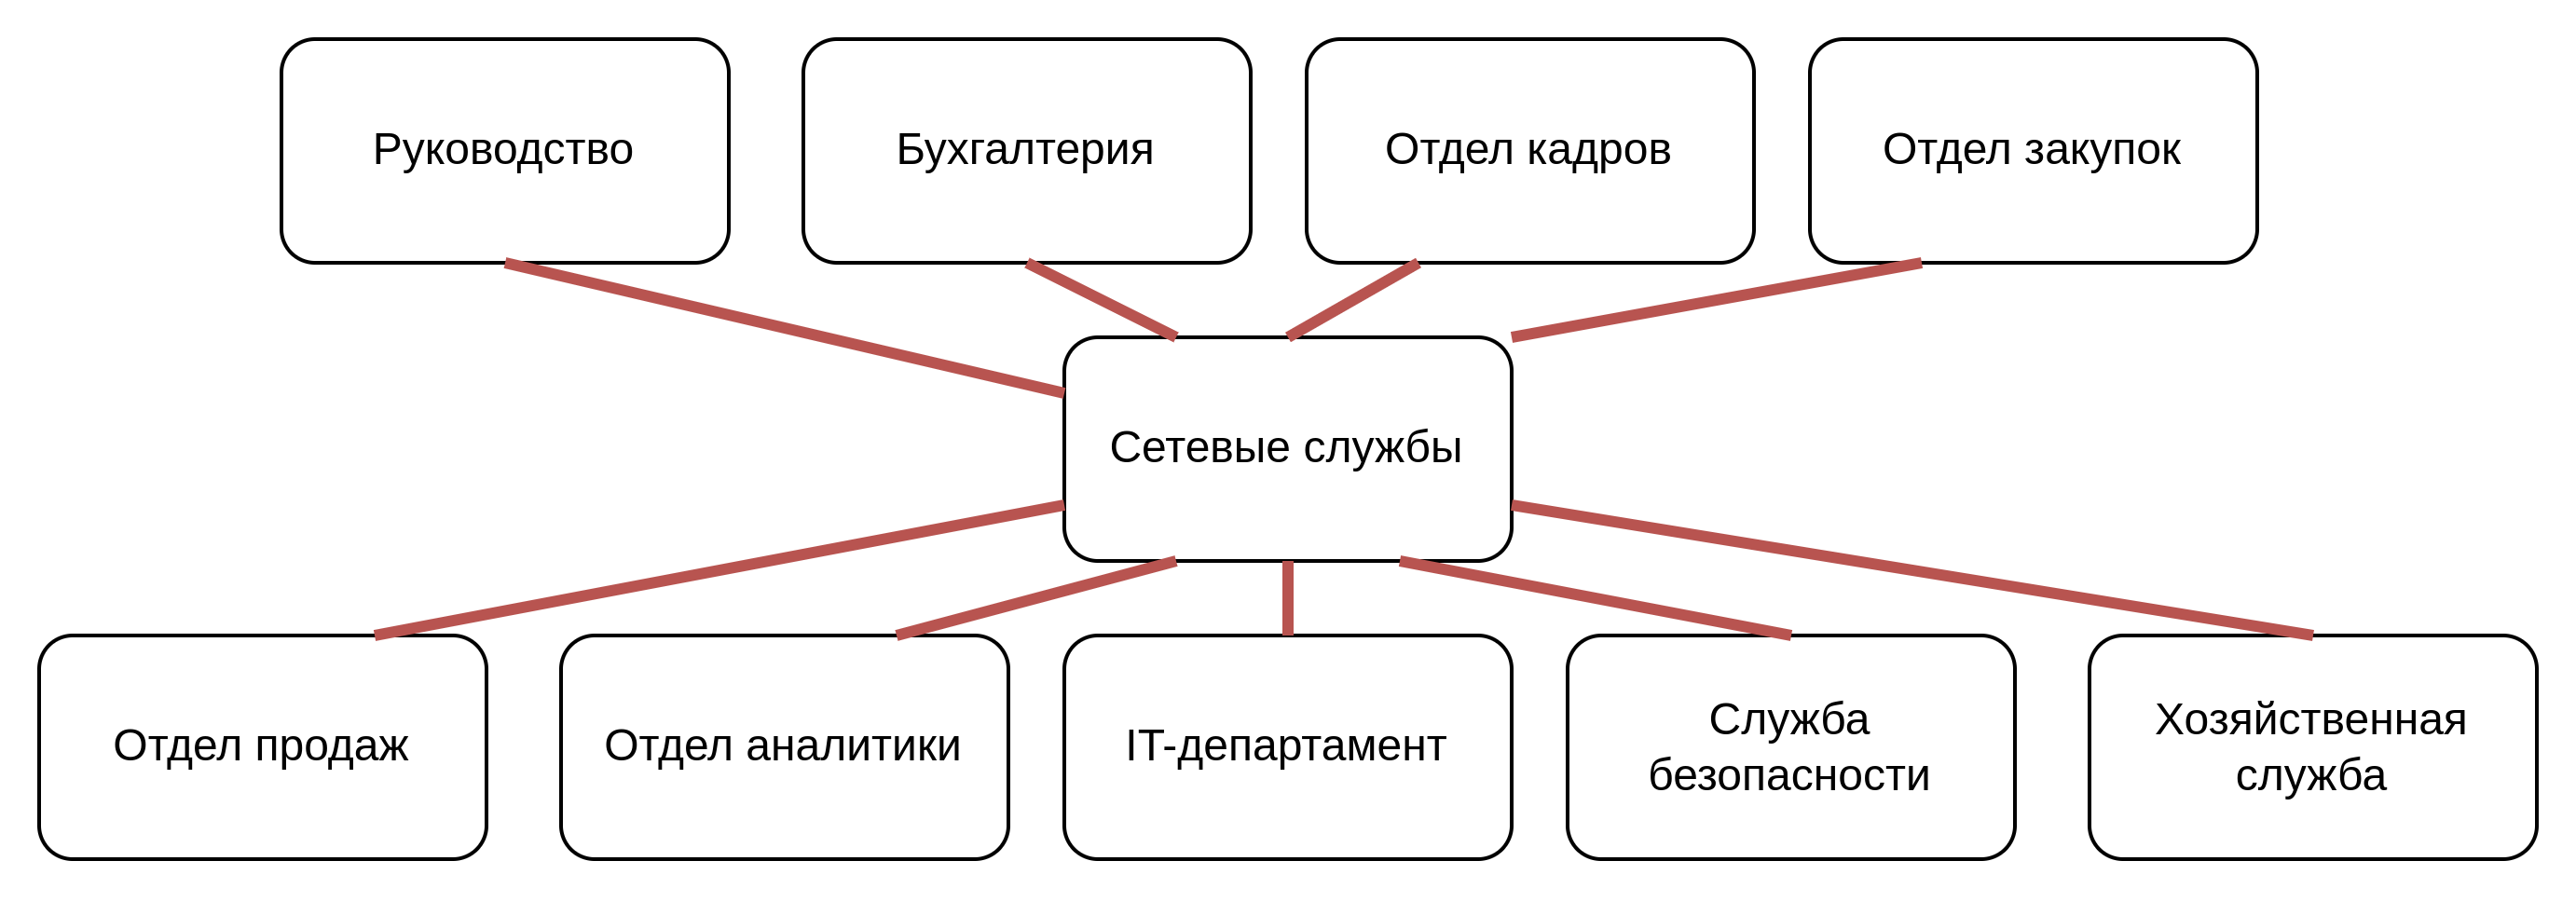
\includegraphics[scale=0.16]{../misc/fieltre.png}
\caption{Схема доступа\label{fig:filtre}}
\end{figure}

% ACL (Access Control List) настроены на всех коммутаторах уровня доступа, кроме SW\_7\_IT\_DERDZYAN. Для всех коммутаторов, кроме SW\_7\_IT\_ DERDZYAN, разрешены входящие пакты только из IP-адреса 192.168.108.0/24 и 192.168.111.0/24. Так же в ACL разрешены IP-адреса из диапазона 192.168.2.0/24, те адреса, которые предназначены для управления устройствами уровня 2.

На основе схемы созданы списки контроля доступа (ACL), которые контролируют и фильтруют взаимодействие и передачу данных между отделами. Такое решение обусловлено тем, что требуемое программное обеспечение для работы сотрудников предприятия установлено на сервере. Для обеспечения дополнительной безопасности отделы, не имеют возможности обмениваться данными между собой. 

На каждом из коммутаторов второго уровня создан список, фильтрующий трафик, который исходя из IP-адреса отправителя пакета на каждом порту определяет допускать трафик или нет. 


\subsection{Планирование политик обеспечения качества обслуживания}
В системе классификации трафика выделены четыре категории: премиальный, золотой, серебряный и бронзовый. Трафик NFS признается и обрабатывается как премиальный. Категория золотого класса включает в себя трафик службы управления пользователями и веб-службы. Серебряный класс охватывает трафик службы динамического конфигурирования хостов, а бронзовый класс связан с трафиком службы доменных имен. Все остальные виды трафика рассматриваются и обрабатываются в соответствии с моделью Best-effort.

Стандартная пересылка используется для узлов, не маркирующих трафик, или для всего остального трафика в данной топологии. Значение поля DSCP IP-пакета устанавливается в 000000 для передачи данных по сети, что гарантирует негарантированную доставку пакетов.

Введены четыре класса моделей поведения с гарантированной пересылкой, каждый из которых размещается в соответствующей очереди. Каждому классу присуща вероятность сброса, и при переполнении очереди пакеты с высокой вероятностью будут отброшены раньше остальных. Предусмотрено три уровня приоритета для отбрасывания.

Основной целью ускоренной пересылки EF является помещение пакетов в очередь с минимальной задержкой и потерями. Для этого используется приоритетная очередь, в которой пакеты отправляются раньше других. Однако существует вероятность блокировки других очередей, поэтому применяется ограничение скорости с использованием контроля. Значения DSCP\cite{dscp-value} обычно обозначаются как EF, в двоичном виде - 101110, а десятичное значение - 46.
% Определено четыре типа класса трафика --- это премиальный, золотой, серебряный и бронзовый. Трафик NFS считается и обрабатывается как премиальный. Трафик золотого класса состоит из трафика службы управления пользователями и веб-службы. Серебряный класс трафика содержит трафик службы динамического конфигурирования хостов, а бронзовый --- это трафик службы доменных имен. Все остальное рассматривается и обрабатывается по модели Best-effort.
%
% Сообщения премиального класса пересылаются с максимальной возможной задержкой до 500 Кбит/с в периоды перегрузки. Класс золотой предпочтительнее	класса серебряного, который в свою очередь, рассматривается предпочтительнее класса бронзового. Классы золотой, серебряный и бронзовый должны иметь 35\%, 25\%, 15\% пропускной способности. Класс бронзовый настроен на 320 Кбит/с, а класс best-effort ограничен 56 Кбит/с.

% Чтобы обеспечивать различные классы трафика, трафик должен быть классифицирован на основе DSCP в домене DiffServ. Для классификации на основе значений DSCP, трафик предварительно помечается соответствующими значениями DSCP во время входа в сеть.
%
% В данной топологии поддержка class selector опущена. Определяется три основные возможные модели поведения: стандартная пересылка (Default Forwarding), гарантированная пересылка (Assumed Forwarding) и экстренная пересылка (Expedited Forwarding).

% Стандартная пересылка используется для узлов, которые не маркируют трафик, либо для всего остального трафика в описываемой топологии. Для передачи данных по сети значения поля DSCP IP-пакета устанавливается в 000000. Данные пакеты с негарантированной доставкой.
%
% Существует 4 класса, модели поведения гарантированная пересылка, и каждый из них будет помещен в свою очередь. Также в каждом классе существует вероятность сброса (drop probability) --- когда очередь заполнена, пакеты с высокой вероятностью отбрасывания будут удалены из очередь раньше других пакетов. Всего есть 3 уровня для приоритета отбрасывания. 
% Поле DSCP делится на две части. Первые 3 бита используются для определения класса (class), а следующие 3 бита используются для определения вероятности сброса (drop probability). Class 4 имеет самый высокий приоритет. Например, любой пакет из class 4 будет обработан лучше, чем пакет из class 3. Значения поля DSCP приведены в Таблице\;\ref{table:some_shit}.
%
%
% \begin{table}[H]
% \centering
% \numberwithin{table}{section}
% \caption{Значения поля DSCP при модели поведения гарантированная доставка\;\label{table:some_shit}}
% \small
% \begin{tabularx}{\textwidth}{|X|X|X|X|X|}
% 	\hline
% 	Вероятность отбрасывания & Класс 1 & Класс 2 & Класс 3 & Класс 4 \\
% 	\hline
% 	Низкая					 & 001010 (10, AF11) & 010010 (18, AF21) & 011010 (26, AF31) & 100010 (34, AF41) \\
% 	\hline
% 	Средняя 				 & 001100 (12, AF12) & 010100 (20, AF22) & 011100 (28, AF32) & 100100 (36, AF42) \\
% 	\hline
% 	Высокая					 & 001110 (14, AF13) & 010110 (22, AF23) & 011110 (30, AF33) & 100110 (38, AF43) \\
% 	\hline
% \end{tabularx}
% \end{table}

% Цель ускоренной пересылки EF --- поместить пакеты в очередь, где они охватывают минимальную задержку и потери пакетов. Для обеспечения этого используется приоритетная очередь (priority queue). Если в очереди с приоритетом есть пакеты, они будут отправлены раньше всех остальных очередей. Но есть вероятность того, что другие очереди не получат возможность отправлять свои пакеты, поэтому выбираются ограничения скорости для этой очереди. Это делается с помощью контроля (polling). Значения DSCP обычно называется EF, в двоичном виде это 101110, десятичное значение 46.

Определенные модели поведения, по которой трафик должен быть обработан и вычисленные значения поля DSCP в Таблице\;\ref{table:some_shit_1}

\begin{table}[H]
\centering
\numberwithin{table}{section}
\caption{Значения DSCP для классов и типов трафика\;\label{table:some_shit_1}}
\small
\begin{tabularx}{\textwidth}{|X|X|X|X|}
	\hline
	Класс трафика & Тип трафика & Модель поведения & Значения DSCP \\
	\hline
	Премиальный 	   & NFS		& EF				& 46 \\
	\hline
	Золотой				& Служба управление пользователями & AF11 & 10 \\
	\cline{2-4}
						& Веб-служба						& AF12 & 12 \\
	\hline
	Серебряный 			& Служба динамического конфигурирования хостов & AF21 & 18 \\
	\hline
	Бронзовый 			& Служба доменных имен							& AF31 & 26 \\
	\hline
\end{tabularx}
\end{table}


\subsection{Планирование службы доменных имен}

DNS сервер для предприятия развернут в рамах программного обеспечения FreeIPA (Free Identity, Policy, Audit), так как он предоставляет интегрированный DNS-сервер. FreeIPA предлагает несколько преимуществ по сравнению с настройкой DNS изолированно:

\begin{enumerate}
	\item Централизованное управление идентификацией: FreeIPA предоставляет единую систему для управления идентификацией, политиками и аудитом. Это означает, что вместе с DNS вы также получаете управление пользователями, группами, хостами и другими объектами в единой системе;
	\item Интеграция с Kerberos и LDAP: FreeIPA включает в себя Kerberos для аутентификации и LDAP для хранения информации о пользователях и политиках. Это позволяет создавать более безопасную и легко масштабируемую сетевую инфраструктуру;
	\item Безопасность: FreeIPA предлагает расширенные функции безопасности, такие как централизованное управление ключами SSH и SSL сертификатами, политики паролей и интеграцию с системами аутентификации многофакторной идентификации;
	\item Автоматизация и упрощение администрирования: FreeIPA позволяет автоматизировать и упрощать многие процессы администрирования, которые при изолированной настройке DNS пришлось бы выполнять вручную.
\end{enumerate}

Были определены и установлены ключевые параметры для настройки DNS-сервера, включая зоны, записи и стратегии отказоустойчивости. После анализа было решено внедрить DNS-сервер с использованием программного обеспечения FreeIPA. Этот выбор обеспечивает интегрированное решение для управления пользователями, политиками и аудитом, дополняя основные DNS-сервисы. Преимущества включают централизованное управление, повышенную безопасность и упрощенное администрирование, что делает FreeIPA предпочтительным выбором для современной инфраструктуры предприятия. 

Результаты планирования службы доменных имен представлены в Таблице\;\ref{table:dns}

\begin{table}[H]
\centering
\numberwithin{table}{section}
\caption{Результаты планирования службы доменных имен\;\label{table:dns}}
\small
\begin{tabularx}{\textwidth}{|X|X|}
\hline
Параметр & Значение параметра \\
\hline
Название зоны & derdzyan.test \\
\hline
Запись в файле зоны & Конфигурируется автоматически программным обеспечением FreeIPA \\
% \hline
% Записи в файле зоны & "dns.derdzyan.test" A 192.168.111.2 \\
% & "dhcp.derdzyan.test" A 192.168.111.3 \\
% & "www.derdzyan.test" A 192.168.111.4 \\
% & "ntp.derdzyan.test" A 192.168.111.5 \\
% & "nfs.derdzyan.test" A 192.168.111.6 \\
% & "server.derdzyan.test" A 192.168.111.7 \\
\hline
Название обратной зоны & 111.168.192.in-addr.arpa. \\
\hline
Запись в файле зоны & Конфигурируется автоматически программным обеспечением FreeIPA \\
% \hline
% Записи в файле обратной зоны & 192.168.111.2 PTR "dns.derdzyan.test" \\
% & 192.168.111.3 PTR "dhcp.derdzyan.test" \\
% & 192.168.111.4 PTR "www.derdzyan.test" \\
% & 192.168.111.5 PTR "ntp.derdzyan.test" \\
% & 192.168.111.6 PTR "nfs.derdzyan.test" \\
% & 192.168.111.7 PTR "server.derdzyan.test" \\
\hline
Список серверов, на которые производится пересылка в случае отсутствия данных на сервере & 1.1.1.1, 8.8.8.8 \\
\hline
\end{tabularx}
\end{table}


\subsection{Планирование политик управления пользователями}

В данном пункте осуществляется планирование политик управления пользователями, сфокусированное на развертывании программного обеспечения FreeIPA. План включает в себя выделение ключевых конфигурационных параметров, необходимых для успешного развертывания данного программного продукта.

Основные конфигурационные параметры включают в себя параметры безопасности, параметры централизованного управления и аудита. Преимущества выбора FreeIPA связаны с его интегрированным решением для управления пользователями, политиками и службой доменных имен DNS (Таблица\;\ref{table:IPA_conf}).

\begin{table}[H]
\centering
\numberwithin{table}{section}
\caption{Основные конфигурационные параметры для FreeIPA\;\label{table:IPA_conf}}
\small
\begin{tabularx}{\textwidth}{|X|X|}
\hline
Название параметр	&	Значение параметра \\ \hline
IP-адрес		  	&	192.168.111.4	\\ \hline
Обратная зона	  	&	111.168.192.in-addr.arpa \\ \hline
Хостнейм сервера	&	server.derdzyan.test \\ \hline
Имя домена			&	server.derdzayn.test \\ \hline
Название зоны		&	derdzyan.test \\ \hline
Сервер пересылки	&	1.1.1.1, 8.8.8.8 \\ \hline
NTP сервер			&	192.168.111.4 \\ \hline
Порт				&	80 \\
\hline
\end{tabularx}
\end{table}


В рамках плана также определены параметры платформы для развертывания программного обеспечения, такие как требуемое количество оперативной памяти, поддерживаемая версия операционной системы, а также необходимые основные параметры и настройки ОС для эффективного функционирования программного обеспечения (Таблица\;\ref{table:IPA_platorm_param}).

\begin{table}[H]
\centering
\numberwithin{table}{section}
\caption{Основные конфигурационные параметры для FreeIPA\;\label{table:IPA_platorm_param}}
\small
\begin{tabularx}{\textwidth}{|X|X|}
\hline
Название параметр & Значение параметра \\ \hline
Оперативная память	&	2ГБ \\ \hline
Процессор			& 	Двухъядерный	\\ \hline
ОС версия			& 	Fedora server 39 (64 bit)	\\ \hline
Постоянная память	&	20ГБ \\
\hline
\end{tabularx}
\end{table}

\subsection{Планирование внедрения DHCP-сервера}

В данном пункте осуществляется планирование конфигурирования DHCP\cite{comp-network-olipher} (Dynamic Host Configuration Protocol), который в автоматическом режиме предоставляет IP-адреса, маски подсетей, шлюзы по умолчанию и другие сетевые параметры в зависимости от конфигураций.

Реализация развертывания сервера осуществлена на сервере предприятия с использованием необходимого пакета – isc-dhcpd version 4.4.3-P1 и изменения конфигурационного файла, в котором необходимо указать диапазон выдаваемых адресов в соответствии с определенной подсетью, стандартное время аренды IP- адреса в секундах, максимально время аренды, шлюз по умолчанию и адрес DNS-сервера.

Планирование распределения адресов по подсетям представлено в Таблице\;\ref{table:dhcp_subnets}

\begin{table}[H]
\centering
\numberwithin{table}{section}
\caption{Результат планирования распределения IP-адресов по отделам\;\label{table:dhcp_subnets}}
\small
\begin{tabularx}{\textwidth}{|X|X|}
\hline
Сегмент сети & Диапазон адресов \\ \hline
192.168.101.0/24 & 192.168.101.2 - 192.168.101.10 \\ \hline
192.168.102.0/24 & 192.168.102.2 - 192.168.102.12 \\ \hline
192.168.103.0/24 & 192.168.103.2 - 192.168.103.12 \\ \hline
192.168.104.0/24 & 192.168.104.2 - 192.168.104.14 \\ \hline
192.168.105.0/24 & 192.168.105.2 - 192.168.105.14 \\ 
\end{tabularx}
\end{table}

\begin{table}[H]
\centering
\numberwithin{table}{section}
\caption{Продолжение Таблицы\;\ref{table:dhcp_subnets}}
\small
\begin{tabularx}{\textwidth}{|X|X|}
\hline
Сегмент сети & Диапазон адресов \\ \hline
192.168.106.0/24 & 192.168.106.2 - 192.168.106.12 \\ \hline
192.168.107.0/24 & 192.168.107.2 - 192.168.107.22 \\ \hline
192.168.108.0/24 & 192.168.108.2 - 192.168.108.3 \\ \hline
192.168.109.0/24 & 192.168.109.2 - 192.168.109.3 \\ \hline
\end{tabularx}
\end{table}

Конечный набор параметров и их значения в рамках планирования DHCP-сервера представлены в Таблице\;\ref{table:dhcp_resault}.

\begin{table}[H]
\centering
\numberwithin{table}{section}
\caption{Результат планирования конфигурации DHCP-сервера\;\label{table:dhcp_resault}}
\small
\begin{tabularx}{\textwidth}{|X|X|}
\hline
Название параметра 			&	Значение параметра \\ \hline
Набор подсетей				&	192.168.101.0 – 192.168.109.0 \\ \hline
Стандартное время аренды	&	6000 секунд \\ \hline
Максимальное время аренды	&	7200 секунд \\ \hline
Шлюз по умолчанию			&	192.168.101.254 – 192.168.109.254 \\ \hline
Адрес DNS сервера			&	109.168.111.4 \\ \hline
\end{tabularx}
\end{table}

Стоит также упомянуть, что при разворачивании DHCP отдельно на сервере, требуется настройка DHCP-relay. Этот компонент перенаправляет запросы DHCP от клиентов через сетевые устройства, такие как маршрутизаторы и коммутаторы, к серверу DHCP. DHCP-relay необходим для обеспечения того, чтобы клиенты могли получать IP-конфигурацию в сетевых архитектурах с множественными подсетями, где прямой широковещательный трафик между подсетями ограничен или невозможен из-за разграничений маршрутизации.

\subsection{Планирование других сетевых служб}

Произведено планирование таких сетевых служб, как NTP (Network Time Protocol), Apache и NFS (Network File System).

Временная служба реализована в составе программного обеспечения chrony, которое состоит из двух компонентов, chronyd - служба, которая в фоновом режиме поддерживает работу времени и chronyc - интерфейс командной строки для chronyd.

Для корректной работы chronyd требуется в первую очередь дополнить конфигурационный файл серверами, которые находятся вблизи локации сервера компании, с которыми будут синхронизироваться часы и указать IP-адреса клиентов, которые могут использовать время на сервере. На клиентской машине в конфигурационном файле задан так же адрес сервера с которым синхронизируются часы клиента.

Apache — веб-сервер, распространяемый бесплатно. Программное обеспечение — кроссплатформенный продукт, то есть работает на разных операционных системах. Основные отличия от конкурентов — надежность и гибкость. Apache\cite{apache-vs-nginx} работает по принципу модулей. Клиент сначала устанавливает ядро, а потом подключает необходимые модули под свои задачи. В рамках конфигурирования сервера Apache в первую очередь добавляется конфигурационный файл, в котором указыается название сервера, путь по которому находится файл со страницей и при необходимости есть возможность установки порта и IP-адреса на которых разворачивается веб-сервер.

Сетевая файловая система (NFS) обеспечивает хранение файлов в сети. Сетевая файловая система (NFS) - это распределенная файловая система. NFS обеспечивает пользователям доступ к файлам, расположенным на удаленных компьютерах, и позволяет работать с этими файлами точно так же, как и с локальными. Например, с помощью команд операционной системы пользователи могут создавать, удалять, считывать, записывать и изменять атрибуты удаленных файлов и каталогов.

В рамках предприятия было решено создать директории на сервере для каждого отдел в <</root>> и разрешить импортирование соответствующим отделам, для этого необходимо каждой новой директории добавить запись в файле конфигурации, задать IP-адрес устройств, которые могут импортировать каталог и дать разрешение на запись и чтение. Так же выделена еще одна директория по пути <</root>>, которая будет уже доступна для всех отделов. Адреса устройств для доступа к директориям будут заданы, как подсети отделов.


\subsection{Определение и расчет сервисной нагрузки}

В данном пункте необходимо оценить нагрузку на сервер, сформированную каждым развернутым сервисом. Необходимо определить медианное и пиковое количество запросов к каждой сетевой службе в течение данного промежутка времени (рабочего дня, рабочей смены, а так же в течение секунды, если это является целесообразным).

Из необходимого трафика, от клиента к серверу, на котором запущены все необходимые службы, необходимо определить и вычислить объем данных одной транзакии (одного запроса) для каждого сервиса с учетом спецификации используемого службой протокола.

На Рисунке\;\ref{fig:NTP_wireshark} представлена транзакция, состоящая из запроса клиента к серверу.

\begin{figure}[H]
\numberwithin{figure}{section}
\centering
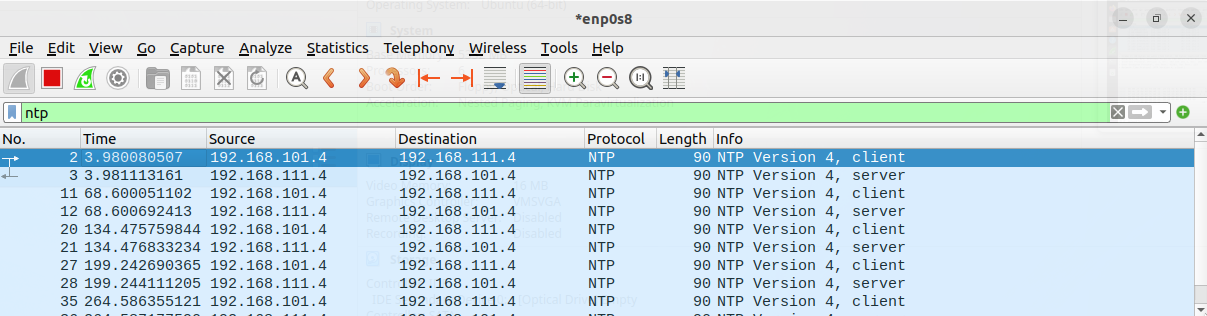
\includegraphics[scale=0.4]{../misc/NTP_wireshark.png}
\caption{Транзакции к NTP\label{fig:NTP_wireshark}}
\end{figure}

При анализе данной транзакции было определено, что количество пакетов в одной транзакции 2, а максимальный размер пакета 720 бит. Требуется определить объем транзакции, воспользовавшись Формулой 1.1


\begin{equation}
\numberwithin{equation}{section}
V_\text{транзакции} = 720 \times 2 = 1440 = 0.002\;\text{Мбит}
\label{eqn:agg_ports}
\end{equation}

Количество обращений к службе времени представлено в Таблице\;\ref{table:NTP_usage}

\begin{table}[H]
\centering
\numberwithin{table}{section}
\caption{Количество обращений к службе времени\;\label{table:NTP_usage}}
\small
\begin{tabularx}{\textwidth}{|X|X|X|X|}
\hline
	Название отдела	&	Количество АРМ	&	Количество обращений за рабочий день	&	Всего пакетов за рабочий день \\ \hline
		Руководство предприятия         & 8       		&  	4000				&	8000  \\
\end{tabularx}
\end{table}

\begin{table}[H]
\centering
\numberwithin{table}{section}
\caption{Продолжение Таблицы\;\ref{table:NTP_usage}}
\small
\begin{tabularx}{\textwidth}{|X|X|X|X|}
\hline
	Название отдела	&	Количество АРМ	&	Количество обращений за рабочий день	&	Всего пакетов за рабочий день \\ \hline
		Бухгалтерия						& 10         	&  	5000				&	10000  \\
		\hline
		Отдел кадров					& 10         	&  	5000				&	10000  \\
        \hline
		Отдел закупок					& 12         	&  	6000				&	12000  \\
        \hline
		Отдел продаж					& 12         	&  	6000				&	12000  \\
        \hline
		Отдел аналитики					& 10         	&  	5000				&	10000  \\
        \hline
		ИТ-департамент					& 20         	&  	10000				&	20000  \\
        \hline
		Служба безопасности				& 1				& 	500					&	1000	  \\
		\hline
		Хозяйственная служба			& 1         	&  	500					&	1000  \\
        \hline
		Итого							& 84			&	42000				& 	84000 \\  
		\hline
\end{tabularx}
\end{table}

В итоге за 9 часов (без вычета обеденного перерыва) формируется примерно 42000 транзакций для файловой службы, то есть около 1.3 транзакции в секунду, что примерно равно 0.0026 Мбит/с. Это значит, что на интерфейс коммутатора только от службы времени будет поступать как минимум 0.0026 Мбит/с трафика или с учетом расчета количества пакетов - 2.6 пакета в секунду.

На Рисунке\;\ref{fig:DNS_wireshark} представлены DNS пакеты, которые отправляются от клиента к серверу и обратно.

\begin{figure}[H]
\numberwithin{figure}{section}
\centering
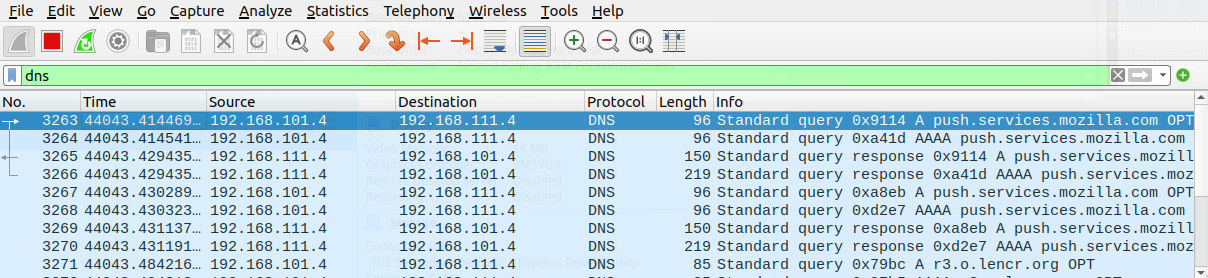
\includegraphics[scale=0.4]{../misc/DNS_wireshark.png}
\caption{Транзакции DNS\label{fig:DNS_wireshark}}
\end{figure}

При анализе данной транзакции определено, что количество пакетов в одной транзакции --- 4, максимальный размер пакета 1632 бита. Объем одной транзакции представлен Формулой 1.2.

\begin{equation}
\numberwithin{equation}{section}
V_\text{транзакции} = 1632 \times 4 = 6528 = 0.006\;\text{Мбит}
\label{eqn:agg_ports}
\end{equation}

Требуется обратить внимание на то, что количество обращений (транзакций) для каждого из отделов взят на основе логических соображений, а не конкретных подсчетов и анализа трафика. Количество обращений к службе доменных имен представлено в Таблиц\;\ref{table:DNS_usage}

\begin{table}[H]
\centering
\numberwithin{table}{section}
\caption{Количество обращений к службе времени\;\label{table:DNS_usage}}
\small
\begin{tabularx}{\textwidth}{|X|X|X|X|}
\hline
	Название отдела	&	Количество АРМ	&	Количество обращений за рабочий день	&	Всего пакетов за рабочий день \\ \hline
		Руководство предприятия         & 8       		&  	16000				&	64000  \\
		\hline
		Бухгалтерия						& 10         	&  	20000				&	80000  \\
        \hline
		Отдел кадров					& 10         	&  	20000				&	80000  \\
        \hline
		Отдел закупок					& 12         	&  	24000				&	96000  \\
        \hline
		Отдел продаж					& 12         	&  	24000				&	96000  \\
        \hline
		Отдел аналитики					& 10         	&  	20000				&	80000  \\
        \hline
		ИТ-департамент					& 20         	&  	40000				&	160000  \\
        \hline
		Служба безопасности				& 1				& 	2000				&	8000	  \\
		\hline
		Хозяйственная служба			& 1         	&  	2000				&	8000  \\
        \hline
		Итого							& 84			&	168000				& 	672000 \\  
		\hline
\end{tabularx}
\end{table}

В итоге за 8-часовой рабочий день формируется примерно 168000 транзакций для файловой службы, то есть около 5.8 транзакций в секунду, что примерно 0.348 Мбит/с. Это значит, что на интерфейс коммутатора только от службы доменных имен будет поступать как минимум 0.348 Мбит/с трафика или с учетом количества пакетов - 23.2 пакета в секунду. 


На Рисунке\;\ref{fig:TCP_HTTP_wireshark} представлены пакеты, отвечающие за соединение клиента в веб-сервером. 
\begin{figure}[H]
\numberwithin{figure}{section}
\centering
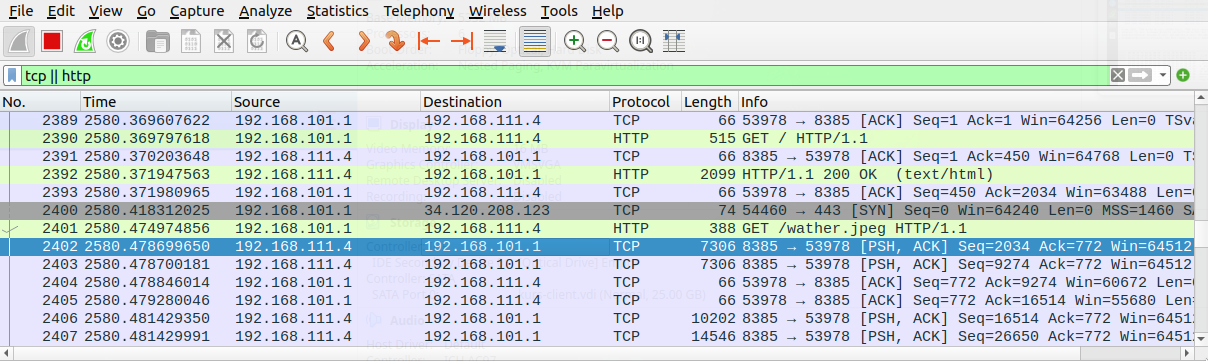
\includegraphics[scale=0.33]{../misc/TCP_HTTP_wireshark.png}
\caption{Результат соединения клиента и веб-сервера\label{fig:TCP_HTTP_wireshark}}
\end{figure}

Соединение состоится на основе применения двух протоколов - TCP и HTTP. При анализе данной транзакции было определено 12 пакетов, максимальный размер пакета 58448 бит. Объем данной транзакции равен (Формула 1.3).

\begin{equation}
\numberwithin{equation}{section}
V_\text{транзакции} = 58448 \times 12 = 701376 = 0.701\;\text{Мбит}
\label{eqn:agg_ports}
\end{equation}

Количество обращений к веб-серверу представлено в Таблиц\;\ref{table:TCP_HTTP_usage}

\begin{table}[H]
\centering
\numberwithin{table}{section}
\caption{Количество обращений к веб-службе\;\label{table:TCP_HTTP_usage}}
\small
\begin{tabularx}{\textwidth}{|X|X|X|X|}
\hline
	Название отдела	&	Количество АРМ	&	Количество обращений за рабочий день	&	Всего пакетов за рабочий день \\ \hline
		Руководство предприятия         & 8       		&  	1600				&	192000  \\
		\hline
		Бухгалтерия						& 10         	&  	7000				&	84000  \\
        \hline
		Отдел кадров					& 10         	&  	7000				&	84000  \\
        \hline
		Отдел закупок					& 12         	&  	7100				&	85200  \\
        \hline
		Отдел продаж					& 12         	&  	7100				&	85200  \\
        \hline
		Отдел аналитики					& 10         	&  	7000				&	84000  \\
        \hline
		ИТ-департамент					& 20         	&  	30000				&	160000  \\
        \hline
		Служба безопасности				& 1				& 	10					&	120	  \\
		\hline
		Хозяйственная служба			& 1         	&  	10					&	120  \\
        \hline
		Итого							& 84			&	66820				& 	801840 \\  
		\hline
\end{tabularx}
\end{table}

В итоге за 8-часовой рабочий день формируется примерно 66820 транзакций для веб-службы, то есть около 2.3 транзакций в секунду, что примерно 1.6 Мбит/с. Это значит, что на интерфейс коммутатора только от веб-службы будет поступать как минимум 1.6 Мбит/с трафика или с учетом количества пакетов - 27.6 пакета в секунду. 

На Рисунке\;\ref{fig:NFS_wireshark} представлены пакеты, отвечающие за NFS трафик. Клиент манипулирует разными pdf, xml файлами размером не больше пяти МБит.
\begin{figure}[H]
\numberwithin{figure}{section}
\centering
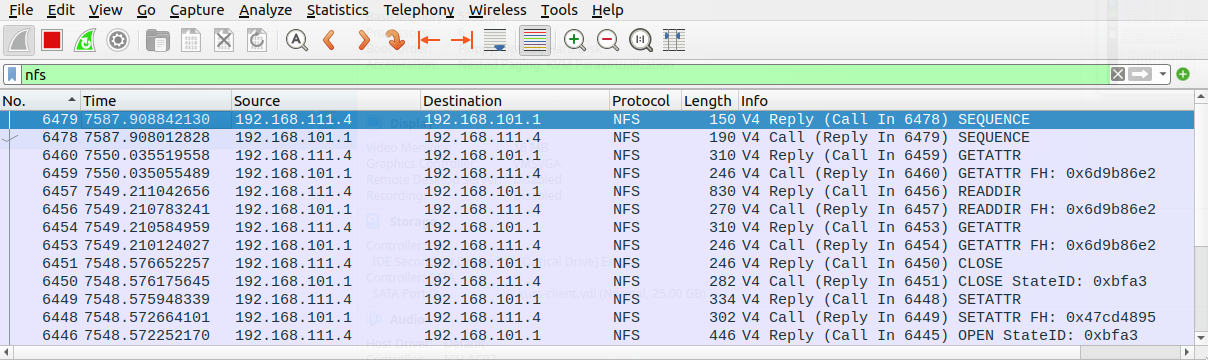
\includegraphics[scale=0.4]{../misc/NFS_wireshark.png}
\caption{Анализ трафика файловой службы\label{fig:NFS_wireshark}}
\end{figure}

При анализе данной транзакции определено, что количество пакетов в одной транзакции --- 540, максимальный размер пакета 2600 бита. Объем одной транзакции представлен Формулой 1.4.


\begin{equation}
\numberwithin{equation}{section}
V_\text{транзакции} = 2600 \times 540 = 1404000 = 1.404\;\text{Мбит}
\label{eqn:agg_ports}
\end{equation}

Количество обращений к файловой службе представлено в Таблиц\;\ref{table:NFS_usage}

\begin{table}[H]
\centering
\numberwithin{table}{section}
\caption{Количество обращений к файловой службе\;\label{table:NFS_usage}}
\small
\begin{tabularx}{\textwidth}{|X|X|X|X|}
\hline
	Название отдела	&	Количество АРМ	&	Количество обращений за рабочий день	&	Всего пакетов за рабочий день \\ \hline
		Руководство предприятия         & 8       		&  	800					&	43200  \\
		\hline
		Бухгалтерия						& 10         	&  	10000				&	5400000  \\
        \hline
		Отдел кадров					& 10         	&  	1000				&	540000  \\
        \hline
		Отдел закупок					& 12         	&  	6000				&	3240000  \\
        \hline
		Отдел продаж					& 12         	&  	6000				&	3240000  \\
        \hline
		Отдел аналитики					& 10         	&  	5000				&	270000  \\
        \hline
		ИТ-департамент					& 20         	&  	8000				&	4320000  \\
        \hline
		Служба безопасности				& 1				& 	10					&	5400	  \\
		\hline
		Хозяйственная служба			& 1         	&  	10					&	5400  \\
        \hline
		Итого							& 84			&	36820				& 	19882800 \\  
		\hline
\end{tabularx}
\end{table}

В итоге за 8-часовой рабочий день формируется примерно 36820 транзакций для файловой службы, то есть около 1.3 транзакций в секунду, что примерно 1.82 Мбит/с. Это значит, что на интерфейс коммутатора только от файловой службы будет поступать как минимум 1.82 Мбит/с трафика или с учетом количества пакетов - 972.8 пакета в секунду. 



На Рисунке\;\ref{fig:DHCP_wireshark} представлены пакеты, относящиеся к службе динамической конфигурации хоста (DHCP). 

\begin{figure}[H]
\numberwithin{figure}{section}
\centering
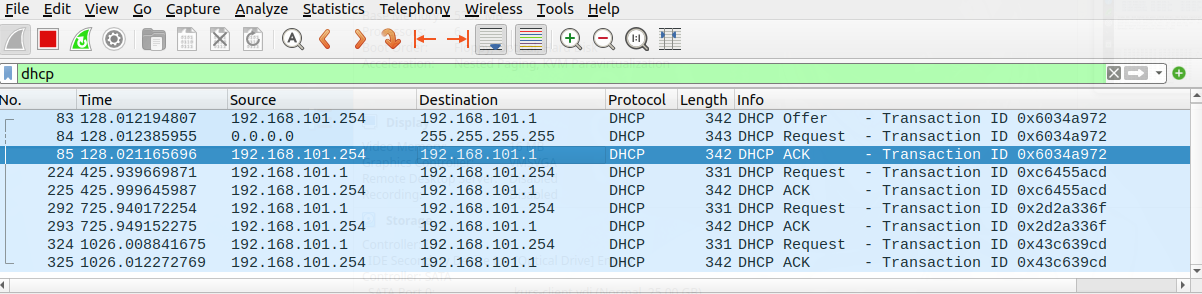
\includegraphics[scale=0.4]{../misc/DHCP_wireshark.png}
\caption{Анализ трафика службы DHCP\label{fig:DHCP_wireshark}}
\end{figure}

При анализе данной транзакции определено, что количество пакетов в одной транзакции --- 12, максимальный размер пакета 2744 бита. Объем одной транзакции представлен Формулой 1.5.

\begin{equation}
\numberwithin{equation}{section}
V_\text{транзакции} = 2744 \times 12  = 32928 = 0.032\;\text{Мбит}
\label{eqn:agg_ports}
\end{equation}

Количество обращений к службе управления пользователям представлено в Таблиц\;\ref{table:DHCP_usage}

\begin{table}[H]
\centering
\numberwithin{table}{section}
\caption{Количество обращений к службе конфигурирования хостов\;\label{table:DHCP_usage}}
\small
\begin{tabularx}{\textwidth}{|X|X|X|X|}
\hline
	Название отдела	&	Количество АРМ	&	Количество обращений за рабочий день	&	Всего пакетов за рабочий день \\ \hline
		Руководство предприятия         & 8       		&  	39				&	468     \\
		\hline
		Бухгалтерия						& 10         	&  	48				&	576		  \\
        \hline
		Отдел кадров					& 10         	&  	48				&	576 \\
        \hline
		Отдел закупок					& 12         	&  	58				&	696  \\
        \hline
		Отдел продаж					& 12         	&  	58				&	696  \\
        \hline
		Отдел аналитики					& 10         	&  	48				&	576  \\
        \hline
		ИТ-департамент					& 20         	&  	96				&	1152  \\
        \hline
		Служба безопасности				& 1				& 	5					&	60	  \\
        \hline
		Хозяйственная служба			& 1         	&  	5					&	60  \\
\end{tabularx}
\end{table}

\begin{table}[H]
\centering
\numberwithin{table}{section}
\caption{Продолжение Таблицы\;\ref{table:DHCP_usage}}
\small
\begin{tabularx}{\textwidth}{|X|X|X|X|}
\hline
	Название отдела	&	Количество АРМ	&	Количество обращений за рабочий день	&	Всего пакетов за рабочий день \\ \hline
		Итого							& 84			&	405				& 	4860 \\  
        \hline
\end{tabularx}
\end{table}

В итоге за 8-часовой рабочий день формируется примерно 4860 транзакций для службы динамической конфигурации хостов, то есть около 1.17 транзакций в секунду, что примерно 0.04 Мбит/с. Это значит, что на интерфейс коммутатора только от службы DHCP поступает как минимум 0.04 Мбит/с трафика или с учетом количества пакетов - 14 пакета в секунду. 



На Рисунке\;\ref{fig:LDAP_wireshark} представлены пакеты, состоящие из аутентификации пользователя в домене FreeIPA, проверки политик доступ (выполнение команд в привилегированном режиме) и другое. 

\begin{figure}[H]
\numberwithin{figure}{section}
\centering
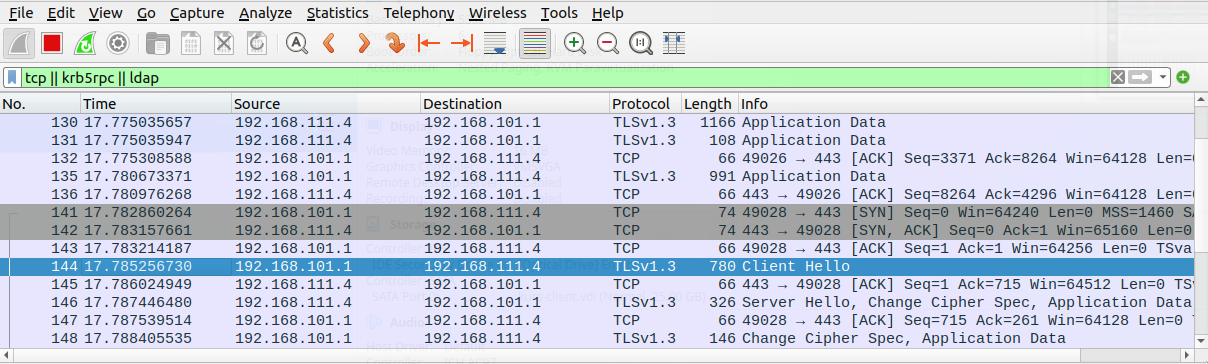
\includegraphics[scale=0.36]{../misc/LDAP_wireshark.png}
\caption{Анализ трафика службы управления пользователями\label{fig:LDAP_wireshark}}
\end{figure}

При анализе данной транзакции определено, что количество пакетов в одной транзакции --- 210, максимальный размер пакета 7936 бита. Объем одной транзакции представлен Формулой 1.6.

\begin{equation}
\numberwithin{equation}{section}
V_\text{транзакции} = 7936 \times 210 = 1666560 = 1.666\;\text{Мбит}
\label{eqn:agg_ports}
\end{equation}

Количество обращений к службе управления пользователям представлено в Таблиц\;\ref{table:IPA_usage}

\begin{table}[H]
\centering
\numberwithin{table}{section}
\caption{Количество обращений к службе управления пользователями\;\label{table:IPA_usage}}
\small
\begin{tabularx}{\textwidth}{|X|X|X|X|}
\hline
	Название отдела	&	Количество АРМ	&	Количество обращений за рабочий день	&	Всего пакетов за рабочий день \\ \hline
		Руководство предприятия         & 8       		&  	2400				&	504000  \\
		\hline
		Бухгалтерия						& 10         	&  	3000				&	630000  \\
        \hline
		Отдел кадров					& 10         	&  	3000				&	630000  \\
        \hline
		Отдел закупок					& 12         	&  	3600				&	756000  \\
        \hline
		Отдел продаж					& 12         	&  	3600				&	756000  \\
        \hline
		Отдел аналитики					& 10         	&  	3000				&	630000  \\
        \hline
		ИТ-департамент					& 20         	&  	20000				&	4200000  \\
		\hline
		Служба безопасности				& 1				& 	200					&	42000	  \\
        \hline
		Хозяйственная служба			& 1         	&  	200					&	42000  \\
        \hline
		Итого							& 84			&	39200				& 	8232000 \\  
		\hline
\end{tabularx}
\end{table}

% \begin{table}[H]
% \centering
% \numberwithin{table}{section}
% \caption{Продолжение Таблицы\;\ref{table:IPA_usage}}
% \small
% \begin{tabularx}{\textwidth}{|X|X|X|X|}
% \hline
% 	Название отдела	&	Количество АРМ	&	Количество обращений за рабочий день	&	Всего пакетов за рабочий день \\ \hline
% \end{tabularx}
% \end{table}

В итоге за 8-часовой рабочий день формируется примерно 39200 транзакций для службы управления пользователями, то есть около 1.36 транзакций в секунду, что примерно 2.26 Мбит/с. Это значит, что на интерфейс коммутатора только от службы управления пользователями поступает как минимум 2.26 Мбит/с трафика или с учетом количества пакетов - 474.5 пакета в секунду. 

На основе полученных данных с использованием и теории очередей M/M/1 произведен расчет минимальной необходимой скорости канала передачи данных между коммутатором L3 и сервером. Исходя из приведенных выше расходов среднее значение максимальных по размеру пакетов равно 15307 сумма всех пакетов передаваемых каждую секунду равна 1489. На основе медианного значения размера пакетов и их количества минимальная скорость канала будет равна 29 Мбит/с (Формула 1.6). Оптимальное значение коэффициента утилизации канала передачи канала взята 80\% так как иначе начинается отбрасывания пакетов, что не является предпочтительным сценарием.

\begin{equation}
\numberwithin{equation}{section}
V_\text{канала} \ge \frac{15307 \times 1489}{0.8} 
\label{eqn:agg_ports}
\end{equation}

Сделан вывод, что канала в 1 Гбит/с хватит для поддерживания необходимой пропускной способности и работы сервисов, как было предложено при предварительном планировании прототипа.


\subsection{Итоговое планирование}

В результате планирования сервисной сети передачи данных предприятия решено, что предварительный прототип полностью соответствует сети и не требует никаких модификаций. Стоит обратить внимание на то, что в доступных устройствах, с учетом модулей расширения, интерфейс с максимальной пропускной способностью имеет тип GigabitEthernet, чего недостаточно для передачи необходимого количества трафика между коммутаторами SW\_1-2\_L3\_DERDZYAN и маршрутизатором. Для обеспечения требуемой скорости передачи данных следует использовать интерфейс 10GigabithEthernet. 

Суммарная стоимость и мощность промежуточных устройств, которые используются в прототипе сети указаны в Таблицах\;\ref{table:oz_price_plan}~---~\ref{table:sk_price_plan}.

\begin{table}[H]
\centering
\numberwithin{table}{section}
\caption{Стоимость и мощность промежуточных устройств для основного здания\;\label{table:oz_price_plan}}
\small
\begin{tabularx}{\textwidth}{|p{3cm}|X|X|X|X|X|}
\hline
	Название устройства		& Количество устройств, шт	& Стоимость одного устройства, у.е. & Мощность одного устройства, Ватт 	& Суммарная стоимость, у.е. & Суммарная мощность, Ватт 	\\ \hline
	Маршрутизатор 4331		& 1							& 3150								& 535								& 3150						& 535						\\ \hline
	Коммутатор L3 3650 24PS & 5							& 5100								& 54								& 25500						& 270						\\ \hline
	Коммутатор 2950T-24		& 7							& 550								& 50								& 3850						& 350						\\ \hline
    \multicolumn{4}{|s|}{Итого:}  & 32500                    & 1155 \\ \hline
\end{tabularx}
\end{table}

\begin{table}[H]
\centering
\numberwithin{table}{section}
\caption{Стоимость и мощность промежуточных устройств для склада\;\label{table:sk_price_plan}}
\small
\begin{tabularx}{\textwidth}{|p{3cm}|X|X|X|X|X|}
\hline
	Название устройства      & Количество устройств, шт & Стоимость одного устройства, у.е. & Мощность одного устройства, Ватт 	& Суммарная стоимость, у.е. & Суммарная мощность, Ватт 	\\ \hline
	Маршрутизатор 1941		 & 1						& 650								& 35								& 650						& 35						\\ \hline
	Коммутатор 1950T-24		 & 1						& 550								& 50								& 550						& 50						\\ \hline
    \multicolumn{4}{|s|}{Итого:}  & 1200                    & 85 \\ \hline
\end{tabularx}
\end{table}

\section{МОДЕЛИРОВАНИЕ СЕТИ}
В данном пункте основное внимание уделяется моделированию сетевой инфраструктуры с использованием соответствующих инструментов. Задача заключается в создании и представлении различных артефактов, отражающих ключевые элементы и характеристики сети. Этот процесс разделяется на два взаимосвязанных этапа.

На первом этапе осуществляется моделирование сервисов, где необходимо разработать и описать основные сервисы, предоставляемые сетью. Это включает четкое определение всех необходимых сервисов, планирование их конфигурации, а также описание взаимодействия этих сервисов между собой и с конечными пользователями.

Второй этап фокусируется на моделировании сети передачи данных. Основное внимание уделяется созданию модели физической и логической структуры сети. Важными аспектами являются разработка топологии сети, включая расположение и связи между устройствами, оценка требуемой пропускной способности и производительности, а также интеграция мер безопасности для обеспечения защиты от несанкционированных утечек данных и аварий.

Комбинированный подход этих двух этапов помогает создать комплексную и эффективную модель сети, которая соответствует всем требованиям и спецификациям, необходимым для успешной реализации и поддержки сетевых функций и сервисов.


\subsection{Моделирование сервисов}

Моделирование сервисов произведено на двух виртуальных машинах с использованием VirualBox.

В качестве сервера используется виртуальная машина под управлением ОС Fedora server 39 с именем локального пользователя --- server\_derdzyan, а в качестве клиента Ubuntu 22.04.3 LTS с именем локального пользователя client\_derdzyan. Результат установки представлен на Рисунке\;\ref{fig:VMs}.

\begin{figure}[H]
\numberwithin{figure}{section}
\centering
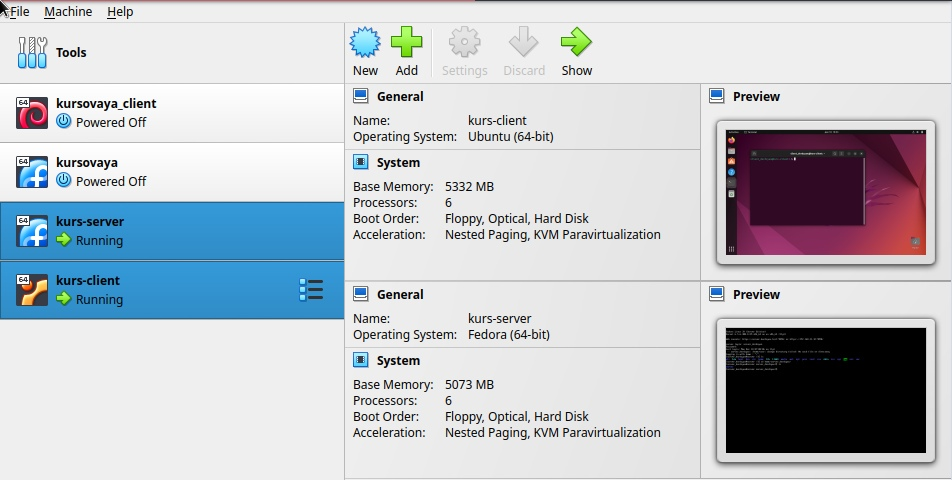
\includegraphics[scale=0.3]{../misc/VMs.jpg}
\caption{Результат установки виртуальных машин\label{fig:VMs}}
\end{figure}

Служба доменных имен развернута в качестве дополнительного пакета программного обеспечения -- FreeIPA. Конфигурация сервера DNS, в качестве доменных зон и DNS записей представлена на Рисунках\;\ref{fig:DNS_zones} -\;\ref{fig:DNS_records}.

\begin{figure}[H]
\numberwithin{figure}{section}
\centering
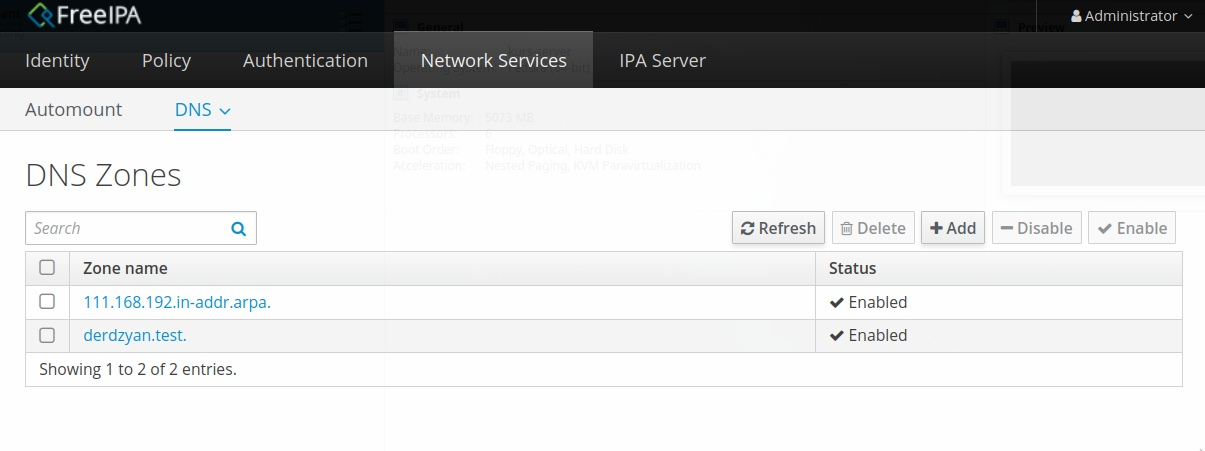
\includegraphics[scale=0.3]{../misc/DNS_zones.jpg}
\caption{DNS зоны\label{fig:DNS_zones}}
\end{figure}

\begin{figure}[H]
\numberwithin{figure}{section}
\centering
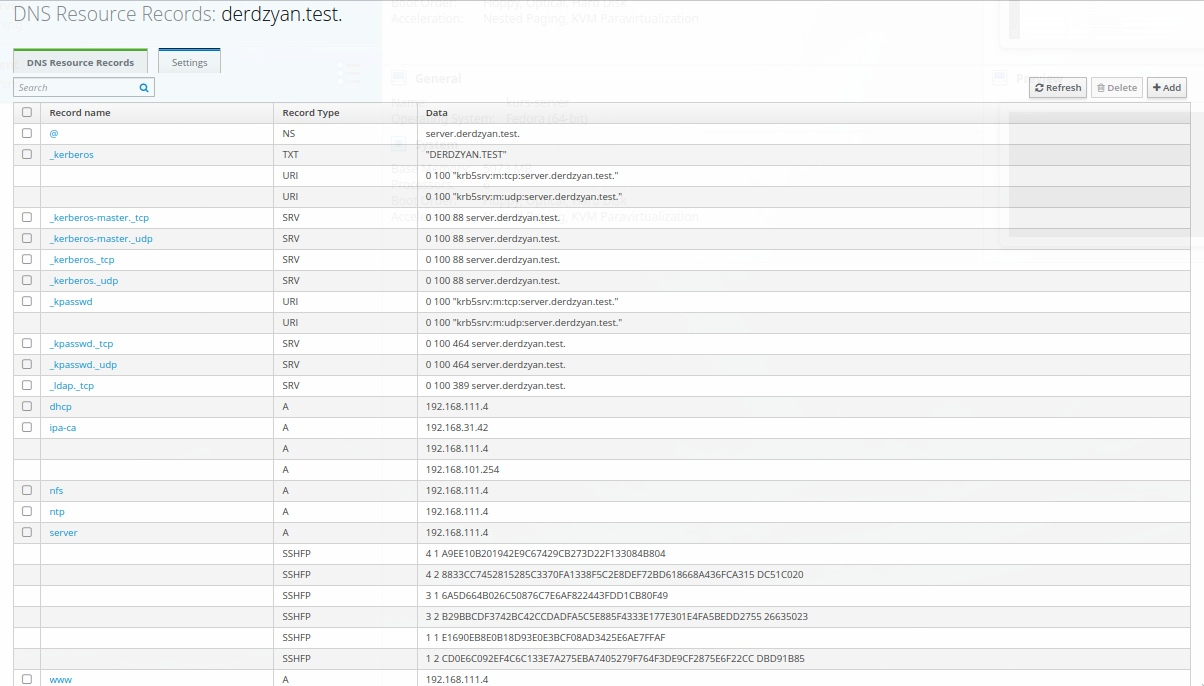
\includegraphics[scale=0.3]{../misc/DNS_records.jpg}
\caption{DNS записи\label{fig:DNS_records}}
\end{figure}

Конфигурация клиента представлена на Рисунке\;\ref{fig:DNS_client_conf}.

\begin{figure}[H]
\numberwithin{figure}{section}
\centering
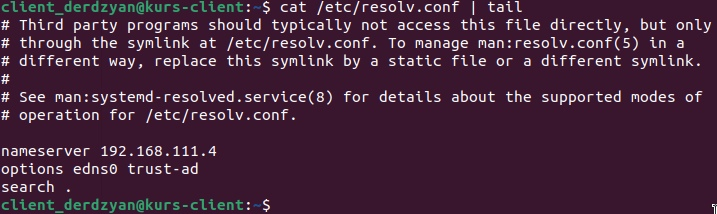
\includegraphics[scale=0.45]{../misc/DNS_client_conf.jpg}
\caption{Конфигурация DNS на клиенте\label{fig:DNS_client_conf}}
\end{figure}

Тестирование DNS с помощью nslookup представлено на Рисунке\;\ref{fig:DNS_client_test}.

\begin{figure}[H]
\numberwithin{figure}{section}
\centering
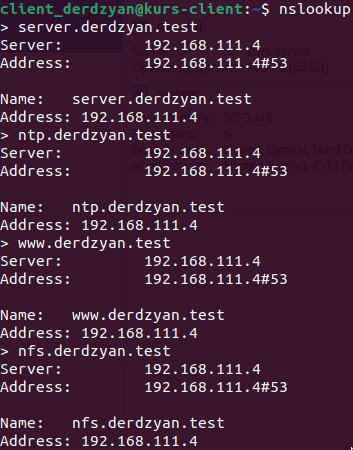
\includegraphics[scale=0.6]{../misc/DNS_client_test.jpg}
\caption{Тестирование DNS\label{fig:DNS_client_test}}
\end{figure}


Далее представлено развертывание службы динамического конфигурирования хостов (DHCP). Конфигураация сервера представлена на Рисунке\;\ref{fig:DHCP_config_server}.

\begin{figure}[H]
\numberwithin{figure}{section}
\centering
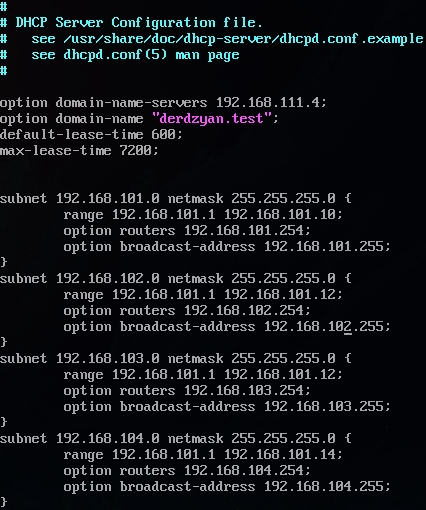
\includegraphics[scale=0.6]{../misc/DHCP_config_server.jpg}
\caption{Конфигурация сервера\label{fig:DHCP_config_server}}
\end{figure}

Конфигурация клиента представлена на Рисунке\;\ref{fig:DHCP_config_client}.

\begin{figure}[H]
\numberwithin{figure}{section}
\centering
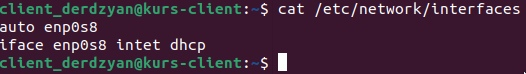
\includegraphics[scale=0.6]{../misc/DHCP_config_client.jpg}
\caption{Конфигурация клиента\label{fig:DHCP_config_client}}
\end{figure}


Результат получения клиентом конфигураций представлена на Рисунке\;\ref{fig:DHCP_res}

\begin{figure}[H]
\numberwithin{figure}{section}
\centering
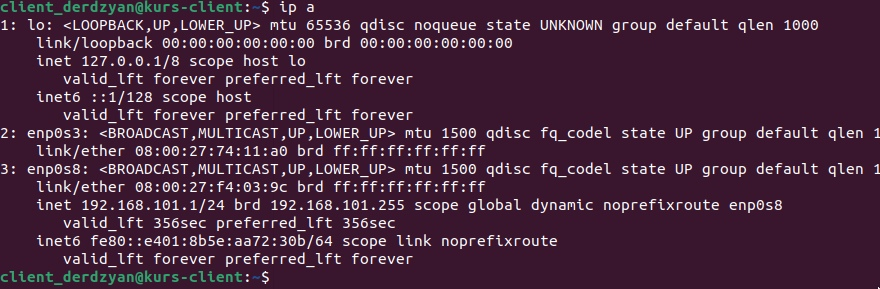
\includegraphics[scale=0.5]{../misc/DHCP_res.jpg}
\caption{Результат получения клиентом конфигурации\label{fig:DHCP_res}}
\end{figure}


Далее представлены артефакты, иллюстрирующие корректное конфигурирование и работы веб-сервера, а именно Apache. На Рисунке\;\ref{fig:apache_server_conf} представлена конфигурация httpd, в котором и указываются параметры для Apache.


\begin{figure}[H]
\numberwithin{figure}{section}
\centering
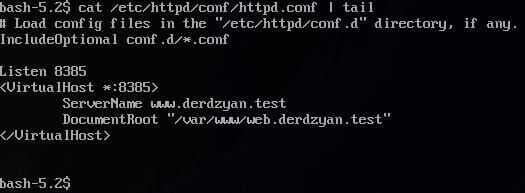
\includegraphics[scale=0.5]{../misc/apache_server_conf.jpg}
\caption{Основной участок конфигурации сервера\label{fig:apache_server_conf}}
\end{figure}

На Рисунке\;\ref{fig:apache_resoult} показана веб-страница предприятия.

\begin{figure}[H]
\numberwithin{figure}{section}
\centering
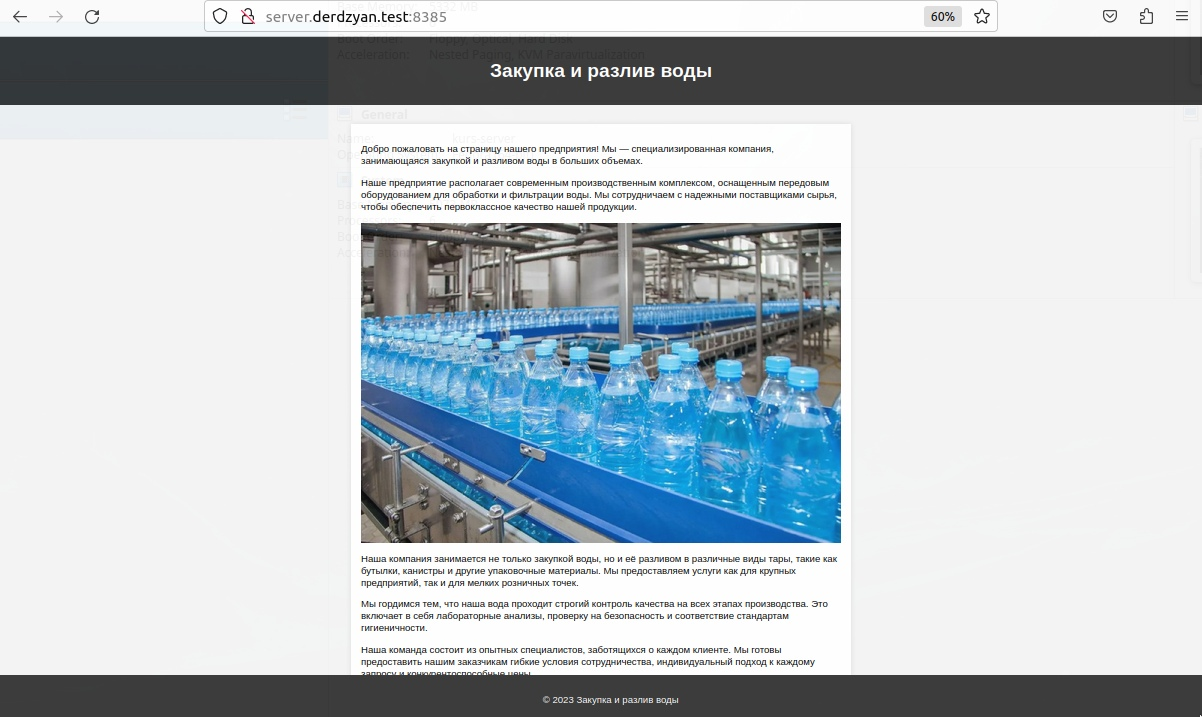
\includegraphics[scale=0.4]{../misc/apache_resoult.jpg}
\caption{Веб-страница\label{fig:apache_resoult}}
\end{figure}

Далее произведено развертывание службы времени --- NTP с использованием chrony. На Рисунке\;\ref{fig:NTP_status_client} представлен статус службы на клиенте.

\begin{figure}[H]
\numberwithin{figure}{section}
\centering
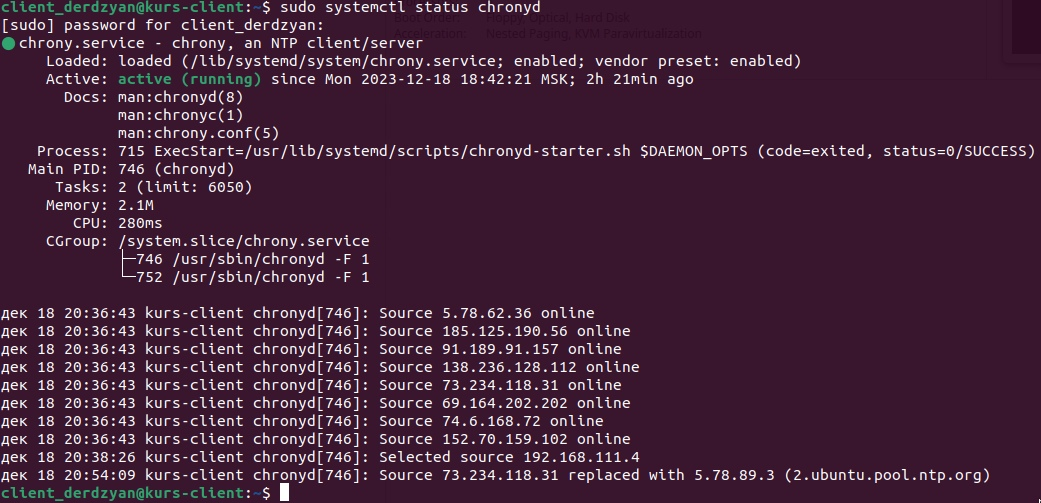
\includegraphics[scale=0.39]{../misc/chronyd_client.jpg}
\caption{Статус службы chronyd на клиенте\label{fig:NTP_status_client}}
\end{figure}

На Рисунке\;\ref{fig:NTP_now_client} представлено текущее время на клиенте.

\begin{figure}[H]
\numberwithin{figure}{section}
\centering
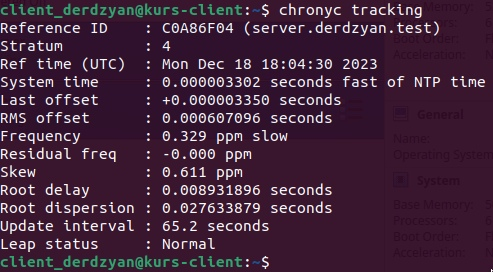
\includegraphics[scale=0.6]{../misc/chronyc_now_client.jpg}
\caption{Текущее время на клиенте\label{fig:NTP_now_client}}
\end{figure}

Следующим выполнено разворачивание файловой службы, используется NFS. На Рисунке\;\ref{fig:NFS_config} представлена конфигурация NFS на сервере.

\begin{figure}[H]
\numberwithin{figure}{section}
\centering
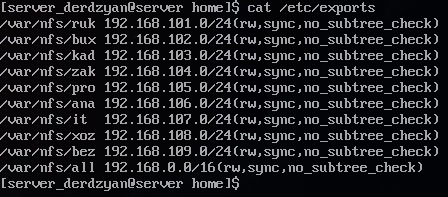
\includegraphics[scale=0.6]{../misc/NFS_config.jpg}
\caption{Конфигурация файловой службы на сервере\label{fig:NFS_config}}
\end{figure}

Проверка доступности файла отправленного с сервера на клиенте, подключенного к директории NFS (Рисунок\;\ref{fig:NFS_client}).

\begin{figure}[H]
\numberwithin{figure}{section}
\centering
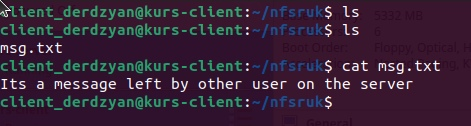
\includegraphics[scale=0.5]{../misc/NFS_client.jpg}
\caption{Проверка доступности файлов на клиенте\label{fig:NFS_client}}
\end{figure}

Также необходимо развернуть службу управления пользователями в качестве ПО – FreeIPA. На Рисунке\;\ref{fig:IPA_status} представлен статус службы FreeIPA.

\begin{figure}[H]
\numberwithin{figure}{section}
\centering
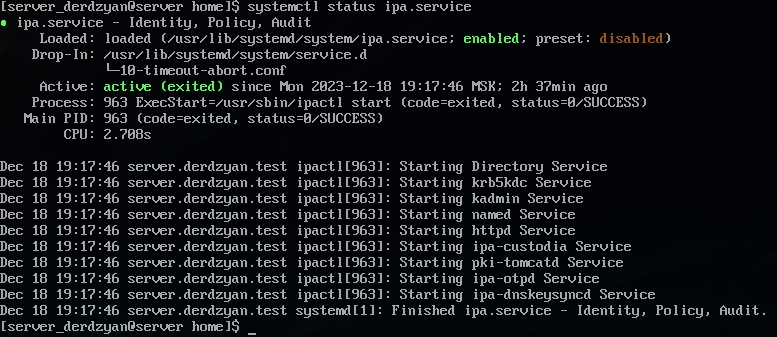
\includegraphics[scale=0.5]{../misc/IPA_status.jpg}
\caption{Статус службы ipa\label{fig:IPA_status}}
\end{figure}

На Рисунке\;\ref{fig:IPA_users} представлены пользователи домена FreeIPA.

\begin{figure}[H]
\numberwithin{figure}{section}
\centering
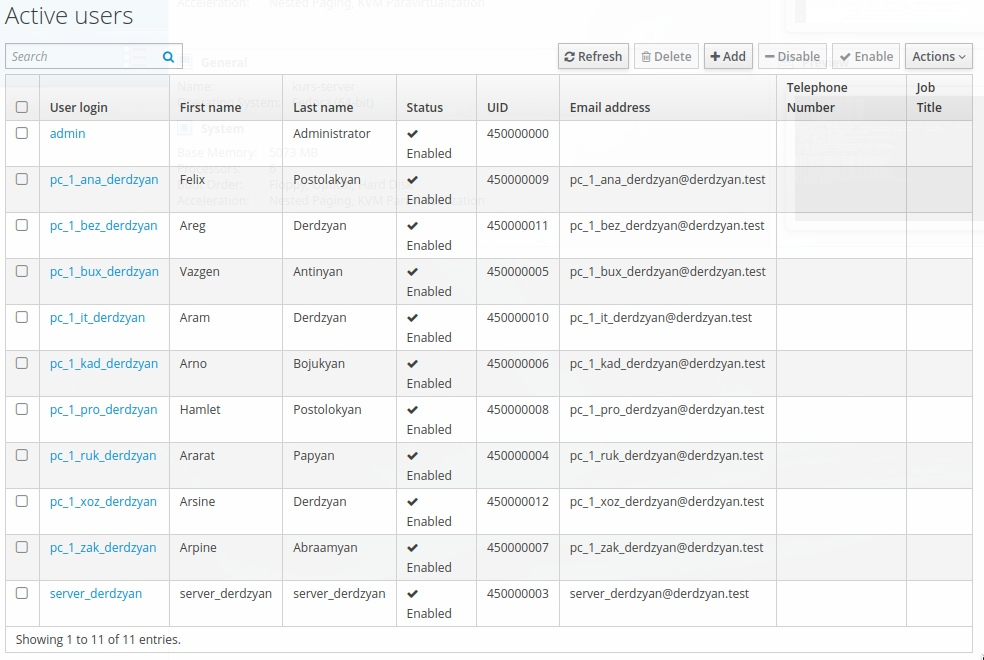
\includegraphics[scale=0.35]{../misc/IPA_users.jpg}
\caption{Пользователи домена FreeIPA\label{fig:IPA_users}}
\end{figure}

На Рисунке\;\ref{fig:IPA_user_log} представлено логирование клиента в домен FreeIPA.

\begin{figure}[H]
\numberwithin{figure}{section}
\centering
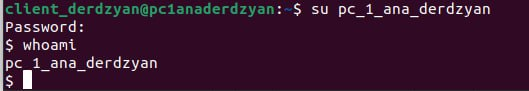
\includegraphics[scale=0.7]{../misc/IPA_user_log.jpg}
\caption{Логирование клиента в домене FreeIPA\label{fig:IPA_user_log}}
\end{figure}



\subsection{Моделирование сети передачи данных}


Моделирование сети передачи данных произведено в стимуляторе сети передачи данных ``Cisco Packet Tracer''. Моделирование сети передачи данных произведено только для основного здания предприятия. Топология содержит указанные выше устройства и приближенные к реальности настройки, которые позволят разным отделам основного здания иметь доступ сетевым службам, в топологии так же реализованы политики качества обслуживания, списки контроля доступа и другое (Рисунок\;\ref{fig:cisco_topo}).

\begin{figure}[H]
\numberwithin{figure}{section}
\centering
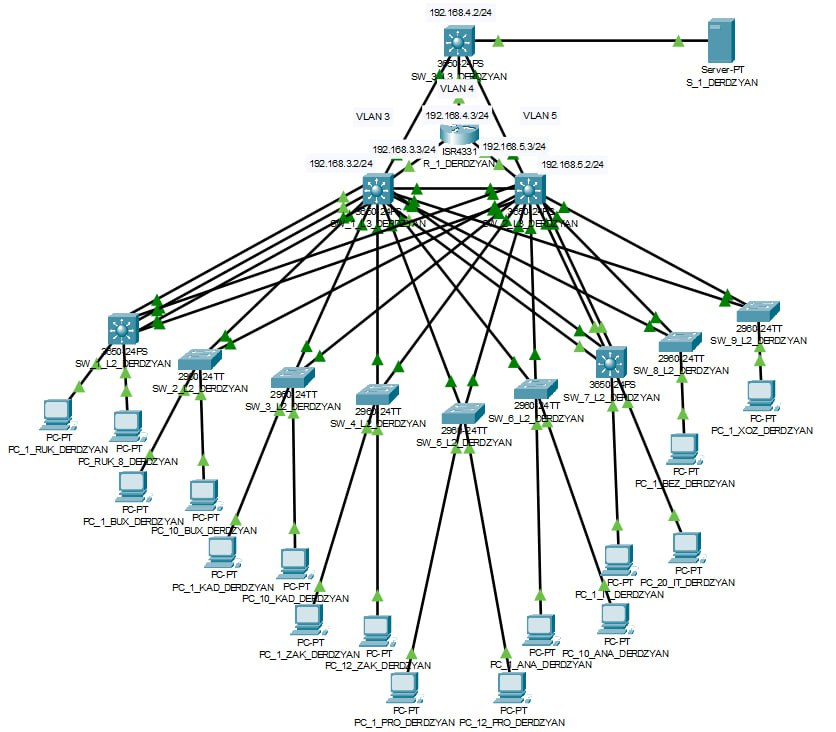
\includegraphics[scale=0.45]{../misc/cisco_topo.png}
\caption{Сконфигурированная топология сети передачи данных\label{fig:cisco_topo}}
\end{figure}

Проверка работоспособности смоделированной сети передачи данных представлена на Рисунке\;\ref{fig:cisco_ping}

\begin{figure}[H]
\numberwithin{figure}{section}
\centering
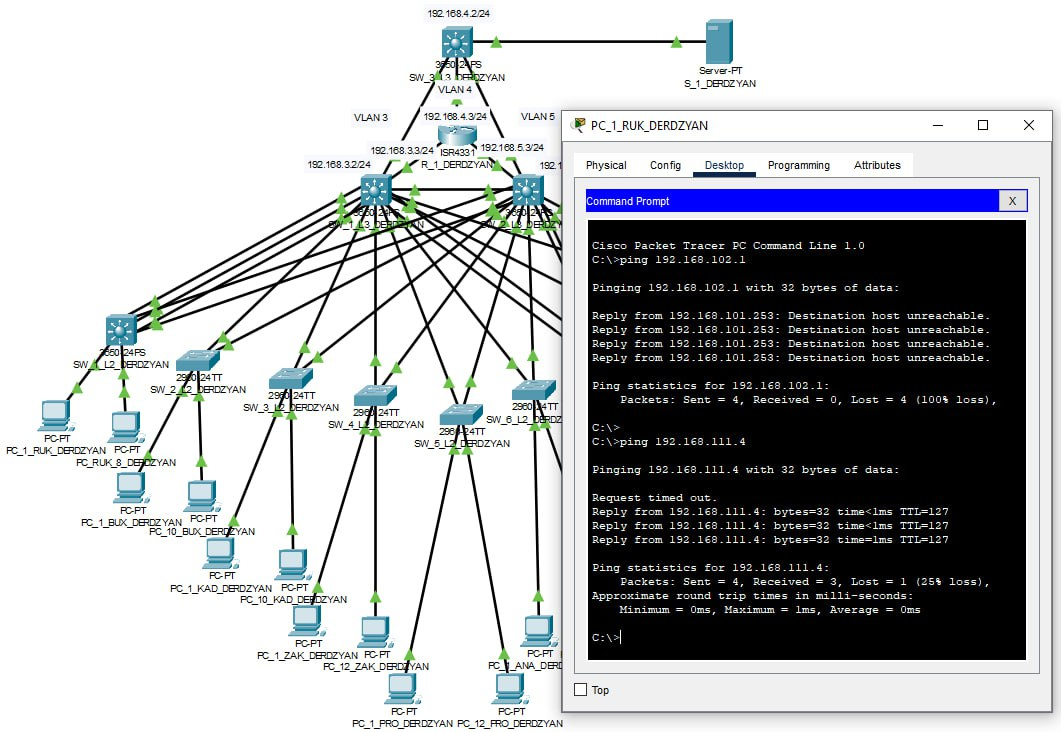
\includegraphics[scale=0.45]{../misc/cisco_ping.png}
\caption{Проверка работоспособности смоделированной сети\label{fig:cisco_ping}}
\end{figure}

В Листинге\;\ref{list:first_conf_into_text} представлена конфигурация одного из коммутаторов уровня три, остальная часть конфигураций приведены в Приложении\;\ref{apx:conf}. В приложении приведены не все конфигурационные файлы, так как большая часть исходят из тех, что приведены за изменением номера порта интерфейса.
\lstinputlisting[caption=Конфигурация устройства SW\_1\_L3\_DERDZYAN\label{list:first_conf_into_text}]{../configs/SW_1_L3_DERDZYAN_startup-config.txt}



% Вот здесь должен быть что то из разряда такого референса на приложение 
%Вот так ссылаться из текста
% Приложении\;\ref{apx:virtualbox}. Конфигурация сетевых устройств 



% \section{ВСЯ ХУЙНЯ}
% Конфигурация маршрутизатора представлена на Листинге \ref{list:ar1}.
% \begin{listing}[H]
% \caption{Конфигурация AR1\label{list:ar1}}
% \begin{Verbatim}[frame=single, fontsize=\footnotesize]
% #
% sysname Huawei
% #
% aaa 
%  authentication-scheme default
%  authorization-scheme default
%  accounting-scheme default
%  domain default 
%  domain default_admin 
%  local-user admin password cipher OOCM4m($F4ajUn1vMEIBNUw#
%  local-user admin service-type http
% #
% firewall zone Local
%  priority 16
% #
% interface Ethernet0/0/0
% #
% interface Ethernet0/0/1
% #
% interface Serial0/0/0
%  link-protocol ppp
% #
% interface Serial0/0/1
%  link-protocol ppp
% #
% interface Serial0/0/2
%  link-protocol ppp
% #
% interface Serial0/0/3
%  link-protocol ppp
% #
% interface GigabitEthernet0/0/0
% \end{Verbatim}
% \end{listing}
% \begin{listing}[H]
% \caption*{Продолжение листинга\;\ref{list:ar1}}
% \begin{Verbatim}[frame=single, fontsize=\footnotesize]
% #
% interface NULL0
% #
% ip route-static 192.168.0.0 255.255.255.192 192.168.110.1
% ip route-static 192.168.0.0 255.255.255.192 192.168.111.1 preference 70
% ip route-static 192.168.0.64 255.255.255.192 192.168.110.1
% ip route-static 192.168.0.64 255.255.255.192 192.168.111.1 preference 70
% ip route-static 192.168.0.128 255.255.255.192 192.168.110.1
% ip route-static 192.168.0.128 255.255.255.192 192.168.111.1 preference 70
% ip route-static 192.168.0.192 255.255.255.224 192.168.110.1
% ip route-static 192.168.0.192 255.255.255.224 192.168.111.1 preference 70
% ip route-static 192.168.0.224 255.255.255.224 192.168.110.1
% ip route-static 192.168.0.224 255.255.255.224 192.168.111.1 preference 70
% ip route-static 192.168.1.0 255.255.255.224 192.168.110.1
% ip route-static 192.168.1.0 255.255.255.224 192.168.111.1 preference 70
% ip route-static 192.168.1.32 255.255.255.240 192.168.110.1
% ip route-static 192.168.1.32 255.255.255.240 192.168.111.1 preference 70
% ip route-static 192.168.1.48 255.255.255.248 192.168.110.1
% ip route-static 192.168.1.48 255.255.255.248 192.168.111.1 preference 70
% ip route-static 192.168.1.56 255.255.255.248 192.168.110.1
% ip route-static 192.168.1.56 255.255.255.248 192.168.111.1 preference 70
% #
% user-interface con 0
% user-interface vty 0 4
% user-interface vty 16 20
% #
% return 
% \end{Verbatim}
% \end{listing}
% \newpage
%
% \begin{listing}[H]
% \caption{Конфигурация SL2-9\label{list:sl2_9}}
% \begin{Verbatim}[frame=single, fontsize=\footnotesize]
%
% #
% sysname Huawei
% #
% vlan batch 11 to 19
% #
% stp mode stp
% #
% cluster enable
% ntdp enable
% ndp enable
% #
% drop illegal-mac alarm
% #
% diffserv domain default
% #
% drop-profile default
% #
% aaa 
% authentication-scheme default
% authorization-scheme default
% accounting-scheme default
% domain default 
% domain default_admin 
% local-user admin password simple admin
% local-user admin service-type http
% #
% interface Vlanif1
% #
% interface MEth0/0/1
% #
% interface GigabitEthernet0/0/1
% port link-type access
% port default vlan 19
% #
% interface GigabitEthernet0/0/2
% port link-type access
% port default vlan 15
% #
% interface GigabitEthernet0/0/3
% port link-type trunk
% port trunk allow-pass vlan 11 to 19
% #
% interface GigabitEthernet0/0/4
% port link-type trunk
% port trunk allow-pass vlan 11 to 19
% #
% interface GigabitEthernet0/0/5
% #
% interface GigabitEthernet0/0/6
% #
% interface GigabitEthernet0/0/7
% #
% interface GigabitEthernet0/0/8
% #
% \end{Verbatim}
% \end{listing}
% \newpage
%
% \lstinputlisting[caption={Конфигурация SL2-10\label{list:sl2_10}}, firstline=1, lastline=43]{misc/config1.txt}
% \newpage
%
% \lstinputlisting[caption={Next}, firstline=51]{misc/config1.txt}
%
\section*{ЗАКЛЮЧЕНИЕ} 
\addcontentsline{toc}{section}{ЗАКЛЮЧЕНИЕ}
В ходе выполнения данной курсовой работы было проведено планирование и реализация сервисной сети передачи данных для предприятия, занимающегося закупкой воды в больших емкостях и последующим разливом в тару меньшего объема. Целью исследования было создание эффективной и надежной сервисной сети передачи данных, удовлетворяющей специфике и требованиям такого типа бизнеса.
Результаты работы позволят обеспечить стабильную и эффективную работу предприятия в долгосрочной перспективе.

Процесс планирования и проектирования сети передачи данных включал в себя анализ исходных данных, определение структуры предприятия, расчет пропускной способности каналов передачи данных, прототипирование сети, а также планирование адресации, маршрутизации, политик фильтрации трафика, обеспечения качества обслуживания, служб доменных имен, управления пользователями, внедрения DHCP-сервера и других сетевых служб.

Инструменты исследования, такие как Cisco Packet Tracer и Apache, обеспечили возможность моделирования и тестирования сетевых архитектур, что способствовало разработке оптимальных решений.

Основными этапами работы стали обзор теоретических основ и современных технологий передачи данных, изучение специфики деятельности предприятия, разработка схемы адресации и маршрутизации, проектирование виртуальных и локальных сетей, создание прототипа, планирование служб и настройка сети, а также проведение расчетов для определения сервисной нагрузки.

Таким образом, выполнение данной курсовой работы позволило разработать рекомендации по проектированию и реализации системы управления закупками и разливом вина для предприятия, занимающегося данной сферой деятельности. Созданная система управления обеспечивает эффективный контроль и управление процессами закупки и разлива, что способствует повышению производительности предприятия. Итоговое решение предоставит предприятию не только возможность улучшить эффективность своей сервисной сети передачи данных, но и станет основой для развития инфраструктуры в будущем.

\begingroup
\let\itshape\upshape
\sloppy
%\raggedright
%\nocite{*} print everything
\printbibliography[title=СПИСОК ИСПОЛЬЗУЕМЫХ ИСТОЧНИКОВ]\addcontentsline{toc}{section}{СПИСОК ИСПОЛЬЗУЕМЫХ ИСТОЧНИКОВ}
\endgroup

%Вот так ссылаться из текста
% Приложении\;\ref{apx:virtualbox}. Конфигурация сетевых устройств 

\clearpage
\section*{ПРИЛОЖЕНИЯ}
\addcontentsline{toc}{section}{ПРИЛОЖЕНИЯ}


\begin{appendices}

\titleformat{name=\section}[display]
	{\newpage\normalfont\centering}
        {\bfseries Приложение\ \thesection}{0em}{}{}
\renewcommand \thesection {\realasbuk{section}}
\addtocontents{toc}{\protect\setcounter{tocdepth}{0}}

\begin{raggedright}
% Приложение\;\ref{apx:qos_acl}~---~Списки контроля доступа для обеспечения политик качества обслуживания\\
% Приложение\;\ref{apx:virtualbox}~---~Моделирование сетевых служб\\ % ну мне это не надо
Приложение\;\ref{apx:conf}~---~Конфигурация сетевых устройств\\
% Приложение\;\ref{apx:test}~---~Тестирование работоспособности сети\\
\end{raggedright}

% \section{Списки контроля доступа для обеспечения политик качества обслуживания}
% \label{apx:qos_acl}
%
% Списки контроля доступа распределы по типам сервисов, на которые будет применяться политики обеспечения качества обслуживания.
%
% Для файловой службы сервера необходима фильтрация портов TCP/UDP 2049 (Листинг\;\ref{list:qos_acl_nfs}).
%
% \begin{lstlisting}[caption=Список контроля доступа для файловой службы\label{list:qos_acl_nfs}]
% ip access-list extended NFS
%  permit tcp host 192.168.109.1 192.168.104.0 0.0.0.255 eq 2049
%  permit udp host 192.168.109.1 192.168.104.0 0.0.0.255 eq 2049
% \end{lstlisting}
%
% Для службы управления пользователями необходима фильтрация по портам TCP/UDP (Листинг\;\ref{list:qos_acl_ipa}), которые используются в рамках данной службы а именно:
%
% TCP порты:
% \begin{itemize}
% \item 80, 443: HTTP/HTTPS;
% \item 389, 636: LDAP/LDAPS;
% \item 88, 464: kerberos;
% \item 53: bind (служба доменных имен).
% \end{itemize}
%
% UDP порты:
% \begin{itemize}
% \item 88, 464: kerberos;
% \item 53: bind (служба доменных имен).
% \end{itemize}
%
% \begin{lstlisting}[caption=Список контроля доступа для службы управления пользователями\label{list:qos_acl_ipa}]
% ip access-list extended IPA
%  permit tcp host 192.168.109.1 192.168.96.0 0.0.15.255 eq 389
%  permit tcp host 192.168.109.1 192.168.96.0 0.0.15.255 eq 636
%  permit tcp host 192.168.109.1 192.168.96.0 0.0.15.255 eq www
%  permit tcp host 192.168.109.1 192.168.96.0 0.0.15.255 eq 443
%  permit tcp host 192.168.109.1 192.168.96.0 0.0.15.255 eq 88
%  permit tcp host 192.168.109.1 192.168.96.0 0.0.15.255 eq 464
%  permit tcp host 192.168.109.1 192.168.96.0 0.0.15.255 eq domain
%  permit udp host 192.168.109.1 192.168.96.0 0.0.15.255 eq 88
%  permit udp host 192.168.109.1 192.168.96.0 0.0.15.255 eq 464
%  permit udp host 192.168.109.1 192.168.96.0 0.0.15.255 eq domain
% \end{lstlisting}
%
% Для списков контроля доступа к веб-службе сервера используется фильтрация по TCP порту 8385, который был выделен как порт веб-страницы (Листинг\;\ref{list:qos_acl_web}).
%
% \begin{lstlisting}[caption=Список контроля доступа для веб-сервера\label{list:qos_acl_web}]
% ip access-list extended WEB
%  permit tcp host 192.168.109.1 192.168.96.0 0.0.15.255 eq 8385
% \end{lstlisting}
%
% Для служб динамического конфигурирования хостов и управления временем также идет фильтрация по стандартным для данных служб UDP портам (Листинги\;\ref{list:qos_acl_dhcp}-\ref{list:qos_acl_ntp}).
%
% \begin{lstlisting}[caption=Список контроля доступа для службы динамического конфигурирования хостов\label{list:qos_acl_dhcp}]
% ip access-list extended DHCP
%  permit udp host 192.168.109.1 192.168.96.0 0.0.15.255 eq bootpc
% \end{lstlisting}
%
% \begin{lstlisting}[caption=Список контроля доступа для службы управления временем\label{list:qos_acl_ntp}]
% ip access-list extended NTP
%  permit udp host 192.168.109.1 192.168.96.0 0.0.15.255 eq 123
% \end{lstlisting}
%
% Поскольку разграничение доступа происходит при помощи отдельных списков контроля доступа, которые установлены на логические интерфейсы VLAN на L3 коммутаторах, то для политик best-effort мы разрешаем все пакеты из любого источника (Листинг\;\ref{list:qos_acl_server}).
%
% \begin{lstlisting}[caption=Список контроля доступа для службы динамического конфигурирования хостов\label{list:qos_acl_server}]
% ip access-list extended SERVER
%  permit ip any any
% \end{lstlisting}
%
% \section{Моделирование сетевых служб}
% \label{apx:virtualbox}


\section{Конфигурация сетевых устройств}
\label{apx:conf}

\lstinputlisting[caption=Конфигурация устройства R\_1\_DERDZYAN\label{list:conf_r1}]{../configs/R_1_DERDZYAN_startup-config.txt}
\lstinputlisting[caption=Конфигурация устройства SW\_2\_L3\_DERDZYAN\label{list:conf_sw2_l3}]{../configs/SW_2_L3_DERDZYAN_startup-config.txt}
\lstinputlisting[caption=Конфигурация устройства SW\_3\_L3\_DERDZYAN\label{list:conf_sw3_l3}]{../configs/SW_3_L3_DERDZYAN_startup-config.txt}
\lstinputlisting[caption=Конфигурация устройства SW\_1\_L2\_DERDZYAN\label{list:conf_sw1_l2}]{../configs/SW_1_L2_DERDZYAN_startup-config.txt}
\lstinputlisting[caption=Конфигурация устройства SW\_2\_L2\_DERDZYAN\label{list:conf_sw2_l2}]{../configs/SW_2_L2_DERDZYAN_startup-config.txt}

% \begin{lstlisting}[caption=Конфигурация устройства R\_1\_IVANOV\label{list:conf_r1}]
% !
% version 15.4
% no service timestamps log datetime msec
% no service timestamps debug datetime msec
% service password-encryption
% !
% hostname R_1_IVANOV
% !
% !
% !
% enable password 7 0822455D0A16
% !
% !
% !
% !
% !
% !
% ip cef
% no ipv6 cef
% !
% !
% !
% username SSHAdmin privilege 15 password 7 0822455D0A16
% !
% !
% !
% !
% !
% !
% !
% !
% ip ssh authentication-retries 2
% ip ssh time-out 60
% no ip domain-lookup
% ip domain-name rtp.ivanov.test
% !
% !
% spanning-tree mode pvst
% !
% !
% !
% !
% !
% !
% interface Loopback0
%  ip address 1.1.1.1 255.255.255.255
% !
% interface GigabitEthernet0/0/0
%  ip address 192.168.116.1 255.255.255.252
%  duplex auto
%  speed auto
% !
% interface GigabitEthernet0/0/1
%  ip address 192.168.112.2 255.255.255.252
%  duplex auto
%  speed auto
% !
% interface GigabitEthernet0/0/2
%  ip address 192.168.113.2 255.255.255.252
%  duplex auto
%  speed auto
% !
% interface Vlan1
%  no ip address
%  shutdown
% !
% router ospf 1
%  log-adjacency-changes
%  network 192.168.112.0 0.0.0.3 area 0
%  network 192.168.113.0 0.0.0.3 area 0
%  network 192.168.116.0 0.0.0.3 area 0
%  default-information originate
% !
% router rip
% !
% ip classless
% ip route 0.0.0.0 0.0.0.0 Loopback0 
% !
% ip flow-export version 9
% !
% !
% !
% banner motd #
% Unauthorized access is prohibited!
% #
% !
% !
% !
% !
% line con 0
%  password 7 0822455D0A16
%  login
% !
% line aux 0
% !
% line vty 0 4
%  password 7 0822455D0A16
%  login local
%  transport input ssh
% line vty 5 14
%  password 7 0822455D0A16
%  login local
%  transport input ssh
% line vty 15
%  login local
%  transport input ssh
% !
% !
% !
% end
%
% \end{lstlisting}
%
% \begin{lstlisting}[caption=Конфигурация устройства R\_2\_IVANOV\label{list:conf_r2}]
% !
% version 15.4
% no service timestamps log datetime msec
% no service timestamps debug datetime msec
% service password-encryption
% !
% hostname R_2_IVANOV
% !
% !
% !
% enable password 7 0822455D0A16
% !
% !
% !
% !
% !
% !
% ip cef
% no ipv6 cef
% !
% !
% !
% username SSHAdmin privilege 15 password 7 0822455D0A16
% !
% !
% !
% !
% !
% !
% !
% !
% ip ssh authentication-retries 2
% ip ssh time-out 60
% no ip domain-lookup
% ip domain-name rtp.ivanov.test
% !
% !
% spanning-tree mode pvst
% !
% !
% !
% !
% !
% !
% interface Loopback0
%  ip address 2.2.2.2 255.255.255.255
% !
% interface GigabitEthernet0/0/0
%  ip address 192.168.116.2 255.255.255.252
%  duplex auto
%  speed auto
% !
% interface GigabitEthernet0/0/1
%  ip address 192.168.115.2 255.255.255.252
%  duplex auto
%  speed auto
% !
% interface GigabitEthernet0/0/2
%  ip address 192.168.114.2 255.255.255.252
%  duplex auto
%  speed auto
% !
% interface Vlan1
%  no ip address
%  shutdown
% !
% router ospf 1
%  log-adjacency-changes
%  network 192.168.114.0 0.0.0.3 area 0
%  network 192.168.115.0 0.0.0.3 area 0
%  network 192.168.116.0 0.0.0.3 area 0
%  default-information originate
% !
% router rip
% !
% ip classless
% ip route 0.0.0.0 0.0.0.0 Loopback0 
% !
% ip flow-export version 9
% !
% !
% !
% banner motd #
% Unauthorized access is prohibited!
% #
% !
% !
% !
% !
% line con 0
%  password 7 0822455D0A16
%  login
% !
% line aux 0
% !
% line vty 0 4
%  password 7 0822455D0A16
%  login local
%  transport input ssh
% line vty 5 14
%  password 7 0822455D0A16
%  login local
%  transport input ssh
% line vty 15
%  login local
%  transport input ssh
% !
% !
% !
% end
%
% \end{lstlisting}
%
% \begin{lstlisting}[caption=Конфигурация устройства SW\_1\_L3\_IVANOV\label{list:conf_sw1_l3}]
% !
% version 16.3.2
% no service timestamps log datetime msec
% no service timestamps debug datetime msec
% service password-encryption
% !
% hostname SW_1_L3_IVANOV
% !
% !
% enable password 7 0822455D0A16
% !
% !
% !
% !
% !
% !
% ip cef
% ip routing
% !
% no ipv6 cef
% !
% !
% !
% username SSHAdmin privilege 15 password 7 0822455D0A16
% !
% !
% !
% !
% !
% !
% !
% !
% !
% !
% ip ssh authentication-retries 2
% ip ssh time-out 60
% no ip domain-lookup
% ip domain-name sw.ivanov.test
% !
% !
% spanning-tree mode pvst
% spanning-tree vlan 101-104,110-112,114 priority 24576
% spanning-tree vlan 105-109,113,115 priority 28672
% !
% class-map match-all EF
%  match access-group name NFS
% class-map match-all platinum
%  match ip dscp ef
% class-map match-all AF11
%  match access-group name IPA
% class-map match-all AF21
%  match access-group name WEB
% class-map match-all gold
%  match ip dscp af11
%  match ip dscp af21
% class-map match-all AF31
%  match access-group name DHCP
% class-map match-all silver
%  match ip dscp af31
% class-map match-all AF41
%  match access-group name NTP
% class-map match-all bronze
%  match ip dscp af31
% class-map match-all best-effort
%  match access-group name SERVER
% !
% policy-map SERVER
%  class platinum
%   priority 500
%  class gold
%   bandwidth percent 35
%  class silver
%   bandwidth percent 25
%  class bronze
%   bandwidth percent 15
%   shape average 320000
%  class best-effort
% !
% policy-map SETDSCP
%  class EF
%   set ip dscp ef
%  class AF11
%   set ip dscp af11
%  class AF21
%   set ip dscp af21
%  class AF31
%   set ip dscp af31
%  class AF41
%   set ip dscp af41
% !
% !
% !
% !
% !
% interface Port-channel1
%  switchport trunk allowed vlan 101-115
%  switchport mode trunk
% !
% interface GigabitEthernet1/0/1
%  switchport trunk allowed vlan 101-115
%  switchport mode trunk
% !
% interface GigabitEthernet1/0/2
%  switchport trunk allowed vlan 101-115
%  switchport mode trunk
% !
% interface GigabitEthernet1/0/3
%  switchport trunk allowed vlan 101-115
%  switchport mode trunk
%  channel-protocol lacp
%  channel-group 1 mode passive
% !
% interface GigabitEthernet1/0/4
%  switchport trunk allowed vlan 101-115
%  switchport mode trunk
%  channel-protocol lacp
%  channel-group 1 mode passive
% !
% interface GigabitEthernet1/0/5
%  switchport trunk allowed vlan 101-115
%  switchport mode trunk
%  channel-protocol lacp
%  channel-group 1 mode passive
% !
% interface GigabitEthernet1/0/6
%  switchport trunk allowed vlan 101-112
%  switchport mode trunk
% !
% interface GigabitEthernet1/0/7
%  switchport trunk allowed vlan 101-115
%  switchport mode trunk
% !
% interface GigabitEthernet1/0/8
%  switchport trunk allowed vlan 101-115
%  switchport mode trunk
% !
% interface GigabitEthernet1/0/9
%  switchport access vlan 112
%  switchport mode access
% !
% interface GigabitEthernet1/0/10
%  switchport access vlan 114
%  switchport mode access
% !
% interface GigabitEthernet1/0/11
%  switchport trunk allowed vlan 101-115
%  switchport mode trunk
% !
% interface GigabitEthernet1/0/12
% !
% interface GigabitEthernet1/0/13
% !
% interface GigabitEthernet1/0/14
% !
% interface GigabitEthernet1/0/15
% !
% interface GigabitEthernet1/0/16
% !
% interface GigabitEthernet1/0/17
% !
% interface GigabitEthernet1/0/18
% !
% interface GigabitEthernet1/0/19
% !
% interface GigabitEthernet1/0/20
% !
% interface GigabitEthernet1/0/21
% !
% interface GigabitEthernet1/0/22
% !
% interface GigabitEthernet1/0/23
% !
% interface GigabitEthernet1/0/24
% !
% interface GigabitEthernet1/1/1
% !
% interface GigabitEthernet1/1/2
% !
% interface GigabitEthernet1/1/3
% !
% interface GigabitEthernet1/1/4
% !
% interface Vlan1
%  no ip address
%  shutdown
% !
% interface Vlan101
%  mac-address 0050.0f51.3701
%  ip address 192.168.101.254 255.255.255.0
%  ip helper-address 192.168.109.1
%  ip access-group IT in
% !
% interface Vlan102
%  mac-address 0050.0f51.3702
%  ip address 192.168.102.254 255.255.255.0
%  ip helper-address 192.168.109.1
%  ip access-group SELLS in
% !
% interface Vlan103
%  mac-address 0050.0f51.3703
%  ip address 192.168.103.254 255.255.255.0
%  ip helper-address 192.168.109.1
%  ip access-group STOCKS in
% !
% interface Vlan104
%  mac-address 0050.0f51.3704
%  ip address 192.168.104.254 255.255.255.0
%  ip helper-address 192.168.109.1
%  ip access-group BUKH in
% !
% interface Vlan105
%  mac-address 0050.0f51.3705
%  ip address 192.168.105.254 255.255.255.0
%  ip helper-address 192.168.109.1
%  ip access-group HR in
% !
% interface Vlan106
%  mac-address 0050.0f51.3706
%  ip address 192.168.106.254 255.255.255.0
%  ip helper-address 192.168.109.1
%  ip access-group HEADS in
% !
% interface Vlan107
%  mac-address 0050.0f51.3707
%  ip address 192.168.107.254 255.255.255.0
%  ip helper-address 192.168.109.1
%  ip access-group AHO in
% !
% interface Vlan108
%  mac-address 0050.0f51.3708
%  ip address 192.168.108.254 255.255.255.0
%  ip helper-address 192.168.109.1
%  ip access-group SEC in
% !
% interface Vlan109
%  mac-address 0050.0f51.3709
%  ip address 192.168.109.254 255.255.255.0
% !
% interface Vlan110
%  mac-address 0050.0f51.370a
%  ip address 192.168.110.254 255.255.255.0
% !
% interface Vlan111
%  mac-address 0050.0f51.370b
%  ip address 192.168.111.1 255.255.255.0
% !
% interface Vlan112
%  mac-address 0050.0f51.370c
%  ip address 192.168.112.1 255.255.255.252
% !
% interface Vlan114
%  mac-address 0050.0f51.370d
%  ip address 192.168.114.1 255.255.255.252
% !
% router ospf 1
%  log-adjacency-changes
%  network 192.168.101.0 0.0.0.255 area 0
%  network 192.168.102.0 0.0.0.255 area 0
%  network 192.168.103.0 0.0.0.255 area 0
%  network 192.168.104.0 0.0.0.255 area 0
%  network 192.168.105.0 0.0.0.255 area 0
%  network 192.168.106.0 0.0.0.255 area 0
%  network 192.168.107.0 0.0.0.255 area 0
%  network 192.168.108.0 0.0.0.255 area 0
%  network 192.168.109.0 0.0.0.255 area 0
%  network 192.168.110.0 0.0.0.255 area 0
%  network 192.168.112.0 0.0.0.3 area 0
%  network 192.168.114.0 0.0.0.3 area 0
% !
% ip classless
% !
% ip flow-export version 9
% !
% !
% ip access-list extended SERVER
%  permit ip any any
% ip access-list extended NFS
%  permit tcp host 192.168.109.1 192.168.104.0 0.0.0.255 eq 2049
%  permit udp host 192.168.109.1 192.168.104.0 0.0.0.255 eq 2049
% ip access-list extended IPA
%  permit tcp host 192.168.109.1 192.168.96.0 0.0.15.255 eq 389
%  permit tcp host 192.168.109.1 192.168.96.0 0.0.15.255 eq 636
%  permit tcp host 192.168.109.1 192.168.96.0 0.0.15.255 eq www
%  permit tcp host 192.168.109.1 192.168.96.0 0.0.15.255 eq 443
%  permit tcp host 192.168.109.1 192.168.96.0 0.0.15.255 eq 88
%  permit tcp host 192.168.109.1 192.168.96.0 0.0.15.255 eq 464
%  permit tcp host 192.168.109.1 192.168.96.0 0.0.15.255 eq domain
%  permit udp host 192.168.109.1 192.168.96.0 0.0.15.255 eq 88
%  permit udp host 192.168.109.1 192.168.96.0 0.0.15.255 eq 464
%  permit udp host 192.168.109.1 192.168.96.0 0.0.15.255 eq domain
% ip access-list extended WEB
%  permit tcp host 192.168.109.1 192.168.96.0 0.0.15.255 eq 8385
% ip access-list extended DHCP
%  permit udp host 192.168.109.1 192.168.96.0 0.0.15.255 eq bootpc
%  permit udp any any eq bootps
% ip access-list extended NTP
%  permit udp host 192.168.109.1 192.168.96.0 0.0.15.255 eq 123
% ip access-list extended SELLS
%  permit ospf any any
%  permit udp any any eq bootps
%  permit udp host 192.168.102.255 host 192.168.109.1 eq bootpc
%  permit ip 192.168.101.0 0.0.0.255 any
%  permit ip 192.168.102.0 0.0.0.255 host 192.168.112.2
%  permit ip 192.168.102.0 0.0.0.255 host 192.168.113.2
%  permit ip 192.168.102.0 0.0.0.255 host 192.168.114.2
%  permit ip 192.168.102.0 0.0.0.255 host 192.168.115.2
%  permit ip 192.168.102.0 0.0.0.255 host 192.168.116.2
%  permit ip 192.168.102.0 0.0.0.255 host 1.1.1.1
%  permit ip 192.168.102.0 0.0.0.255 host 2.2.2.2
%  permit icmp 192.168.102.0 0.0.0.255 host 192.168.109.1 echo
%  permit icmp 192.168.102.0 0.0.0.255 host 192.168.109.1 echo-reply
%  permit tcp 192.168.102.0 0.0.0.255 host 192.168.109.1 eq domain
%  permit tcp 192.168.102.0 0.0.0.255 host 192.168.109.1 eq www
%  permit udp 192.168.102.0 0.0.0.255 host 192.168.109.1 eq domain
%  permit tcp 192.168.102.0 0.0.0.255 host 192.168.109.1 eq 389
%  permit tcp 192.168.102.0 0.0.0.255 host 192.168.109.1 eq 636
%  permit tcp 192.168.102.0 0.0.0.255 host 192.168.109.1 eq 88
%  permit tcp 192.168.102.0 0.0.0.255 host 192.168.109.1 eq 464
%  permit tcp 192.168.102.0 0.0.0.255 host 192.168.109.1 eq 2049
%  permit tcp 192.168.102.0 0.0.0.255 host 192.168.109.1 eq 8385
%  permit udp 192.168.102.0 0.0.0.255 host 192.168.109.1 eq 123
%  permit udp 192.168.102.0 0.0.0.255 host 192.168.109.1 eq 88
%  permit udp 192.168.102.0 0.0.0.255 host 192.168.109.1 eq 464
%  permit udp 192.168.102.0 0.0.0.255 host 192.168.109.1 eq 2049
% ip access-list extended STOCKS
%  permit ospf any any
%  permit udp any any eq bootps
%  permit udp host 192.168.103.255 host 192.168.109.1 eq bootpc
%  permit ip 192.168.101.0 0.0.0.255 any
%  permit ip 192.168.103.0 0.0.0.255 host 192.168.112.2
%  permit ip 192.168.103.0 0.0.0.255 host 192.168.113.2
%  permit ip 192.168.103.0 0.0.0.255 host 192.168.114.2
%  permit ip 192.168.103.0 0.0.0.255 host 192.168.115.2
%  permit ip 192.168.103.0 0.0.0.255 host 192.168.116.2
%  permit ip 192.168.103.0 0.0.0.255 host 1.1.1.1
%  permit ip 192.168.103.0 0.0.0.255 host 2.2.2.2
%  permit icmp 192.168.103.0 0.0.0.255 host 192.168.109.1 echo
%  permit icmp 192.168.103.0 0.0.0.255 host 192.168.109.1 echo-reply
%  permit tcp 192.168.103.0 0.0.0.255 host 192.168.109.1 eq domain
%  permit tcp 192.168.103.0 0.0.0.255 host 192.168.109.1 eq www
%  permit udp 192.168.103.0 0.0.0.255 host 192.168.109.1 eq domain
%  permit tcp 192.168.103.0 0.0.0.255 host 192.168.109.1 eq 389
%  permit tcp 192.168.103.0 0.0.0.255 host 192.168.109.1 eq 636
%  permit tcp 192.168.103.0 0.0.0.255 host 192.168.109.1 eq 88
%  permit tcp 192.168.103.0 0.0.0.255 host 192.168.109.1 eq 464
%  permit tcp 192.168.103.0 0.0.0.255 host 192.168.109.1 eq 2049
%  permit tcp 192.168.103.0 0.0.0.255 host 192.168.109.1 eq 8385
%  permit udp 192.168.103.0 0.0.0.255 host 192.168.109.1 eq 123
%  permit udp 192.168.103.0 0.0.0.255 host 192.168.109.1 eq 88
%  permit udp 192.168.103.0 0.0.0.255 host 192.168.109.1 eq 464
%  permit udp 192.168.103.0 0.0.0.255 host 192.168.109.1 eq 2049
% ip access-list extended BUKH
%  permit ospf any any
%  permit udp any any eq bootps
%  permit udp host 192.168.104.255 host 192.168.109.1 eq bootpc
%  permit ip 192.168.101.0 0.0.0.255 any
%  permit ip 192.168.104.0 0.0.0.255 host 192.168.112.2
%  permit ip 192.168.104.0 0.0.0.255 host 192.168.113.2
%  permit ip 192.168.104.0 0.0.0.255 host 192.168.114.2
%  permit ip 192.168.104.0 0.0.0.255 host 192.168.115.2
%  permit ip 192.168.104.0 0.0.0.255 host 192.168.116.2
%  permit ip 192.168.104.0 0.0.0.255 host 1.1.1.1
%  permit ip 192.168.104.0 0.0.0.255 host 2.2.2.2
%  permit icmp 192.168.104.0 0.0.0.255 host 192.168.109.1 echo
%  permit icmp 192.168.104.0 0.0.0.255 host 192.168.109.1 echo-reply
%  permit tcp 192.168.104.0 0.0.0.255 host 192.168.109.1 eq domain
%  permit tcp 192.168.104.0 0.0.0.255 host 192.168.109.1 eq www
%  permit udp 192.168.104.0 0.0.0.255 host 192.168.109.1 eq domain
%  permit tcp 192.168.104.0 0.0.0.255 host 192.168.109.1 eq 389
%  permit tcp 192.168.104.0 0.0.0.255 host 192.168.109.1 eq 636
%  permit tcp 192.168.104.0 0.0.0.255 host 192.168.109.1 eq 88
%  permit tcp 192.168.104.0 0.0.0.255 host 192.168.109.1 eq 464
%  permit tcp 192.168.104.0 0.0.0.255 host 192.168.109.1 eq 2049
%  permit tcp 192.168.104.0 0.0.0.255 host 192.168.109.1 eq 8385
%  permit udp 192.168.104.0 0.0.0.255 host 192.168.109.1 eq 123
%  permit udp 192.168.104.0 0.0.0.255 host 192.168.109.1 eq 88
%  permit udp 192.168.104.0 0.0.0.255 host 192.168.109.1 eq 464
%  permit udp 192.168.104.0 0.0.0.255 host 192.168.109.1 eq 2049
% ip access-list extended HR
%  permit ospf any any
%  permit udp any any eq bootps
%  permit udp host 192.168.105.255 host 192.168.109.1 eq bootpc
%  permit ip 192.168.101.0 0.0.0.255 any
%  permit ip 192.168.105.0 0.0.0.255 host 192.168.112.2
%  permit ip 192.168.105.0 0.0.0.255 host 192.168.113.2
%  permit ip 192.168.105.0 0.0.0.255 host 192.168.114.2
%  permit ip 192.168.105.0 0.0.0.255 host 192.168.115.2
%  permit ip 192.168.105.0 0.0.0.255 host 192.168.116.2
%  permit ip 192.168.105.0 0.0.0.255 host 1.1.1.1
%  permit ip 192.168.105.0 0.0.0.255 host 2.2.2.2
%  permit icmp 192.168.105.0 0.0.0.255 host 192.168.109.1 echo
%  permit icmp 192.168.105.0 0.0.0.255 host 192.168.109.1 echo-reply
%  permit tcp 192.168.105.0 0.0.0.255 host 192.168.109.1 eq domain
%  permit tcp 192.168.105.0 0.0.0.255 host 192.168.109.1 eq www
%  permit udp 192.168.105.0 0.0.0.255 host 192.168.109.1 eq domain
%  permit tcp 192.168.105.0 0.0.0.255 host 192.168.109.1 eq 389
%  permit tcp 192.168.105.0 0.0.0.255 host 192.168.109.1 eq 636
%  permit tcp 192.168.105.0 0.0.0.255 host 192.168.109.1 eq 88
%  permit tcp 192.168.105.0 0.0.0.255 host 192.168.109.1 eq 464
%  permit tcp 192.168.105.0 0.0.0.255 host 192.168.109.1 eq 2049
%  permit tcp 192.168.105.0 0.0.0.255 host 192.168.109.1 eq 8385
%  permit udp 192.168.105.0 0.0.0.255 host 192.168.109.1 eq 123
%  permit udp 192.168.105.0 0.0.0.255 host 192.168.109.1 eq 88
%  permit udp 192.168.105.0 0.0.0.255 host 192.168.109.1 eq 464
%  permit udp 192.168.105.0 0.0.0.255 host 192.168.109.1 eq 2049
% ip access-list extended HEADS
%  permit ospf any any
%  permit udp any any eq bootps
%  permit udp host 192.168.106.255 host 192.168.109.1 eq bootpc
%  permit ip 192.168.101.0 0.0.0.255 any
%  permit ip 192.168.106.0 0.0.0.255 host 192.168.112.2
%  permit ip 192.168.106.0 0.0.0.255 host 192.168.113.2
%  permit ip 192.168.106.0 0.0.0.255 host 192.168.114.2
%  permit ip 192.168.106.0 0.0.0.255 host 192.168.115.2
%  permit ip 192.168.106.0 0.0.0.255 host 192.168.116.2
%  permit ip 192.168.106.0 0.0.0.255 host 1.1.1.1
%  permit ip 192.168.106.0 0.0.0.255 host 2.2.2.2
%  permit icmp 192.168.106.0 0.0.0.255 host 192.168.109.1 echo
%  permit icmp 192.168.106.0 0.0.0.255 host 192.168.109.1 echo-reply
%  permit tcp 192.168.106.0 0.0.0.255 host 192.168.109.1 eq domain
%  permit tcp 192.168.106.0 0.0.0.255 host 192.168.109.1 eq www
%  permit udp 192.168.106.0 0.0.0.255 host 192.168.109.1 eq domain
%  permit tcp 192.168.106.0 0.0.0.255 host 192.168.109.1 eq 389
%  permit tcp 192.168.106.0 0.0.0.255 host 192.168.109.1 eq 636
%  permit tcp 192.168.106.0 0.0.0.255 host 192.168.109.1 eq 88
%  permit tcp 192.168.106.0 0.0.0.255 host 192.168.109.1 eq 464
%  permit tcp 192.168.106.0 0.0.0.255 host 192.168.109.1 eq 2049
%  permit tcp 192.168.106.0 0.0.0.255 host 192.168.109.1 eq 8385
%  permit udp 192.168.106.0 0.0.0.255 host 192.168.109.1 eq 123
%  permit udp 192.168.106.0 0.0.0.255 host 192.168.109.1 eq 88
%  permit udp 192.168.106.0 0.0.0.255 host 192.168.109.1 eq 464
%  permit udp 192.168.106.0 0.0.0.255 host 192.168.109.1 eq 2049
% ip access-list extended AHO
%  permit ospf any any
%  permit udp any any eq bootps
%  permit udp host 192.168.107.255 host 192.168.109.1 eq bootpc
%  permit ip 192.168.101.0 0.0.0.255 any
%  permit ip 192.168.107.0 0.0.0.255 host 192.168.112.2
%  permit ip 192.168.107.0 0.0.0.255 host 192.168.113.2
%  permit ip 192.168.107.0 0.0.0.255 host 192.168.114.2
%  permit ip 192.168.107.0 0.0.0.255 host 192.168.115.2
%  permit ip 192.168.107.0 0.0.0.255 host 192.168.116.2
%  permit ip 192.168.107.0 0.0.0.255 host 1.1.1.1
%  permit ip 192.168.107.0 0.0.0.255 host 2.2.2.2
%  permit icmp 192.168.107.0 0.0.0.255 host 192.168.109.1 echo
%  permit icmp 192.168.107.0 0.0.0.255 host 192.168.109.1 echo-reply
%  permit tcp 192.168.107.0 0.0.0.255 host 192.168.109.1 eq domain
%  permit tcp 192.168.107.0 0.0.0.255 host 192.168.109.1 eq www
%  permit udp 192.168.107.0 0.0.0.255 host 192.168.109.1 eq domain
%  permit tcp 192.168.107.0 0.0.0.255 host 192.168.109.1 eq 389
%  permit tcp 192.168.107.0 0.0.0.255 host 192.168.109.1 eq 636
%  permit tcp 192.168.107.0 0.0.0.255 host 192.168.109.1 eq 88
%  permit tcp 192.168.107.0 0.0.0.255 host 192.168.109.1 eq 464
%  permit tcp 192.168.107.0 0.0.0.255 host 192.168.109.1 eq 2049
%  permit tcp 192.168.107.0 0.0.0.255 host 192.168.109.1 eq 8385
%  permit udp 192.168.107.0 0.0.0.255 host 192.168.109.1 eq 123
%  permit udp 192.168.107.0 0.0.0.255 host 192.168.109.1 eq 88
%  permit udp 192.168.107.0 0.0.0.255 host 192.168.109.1 eq 464
%  permit udp 192.168.107.0 0.0.0.255 host 192.168.109.1 eq 2049
% ip access-list extended SEC
%  permit ospf any any
%  permit udp any any eq bootps
%  permit udp host 192.168.108.255 host 192.168.109.1 eq bootpc
%  permit ip 192.168.101.0 0.0.0.255 any
%  permit ip 192.168.108.0 0.0.0.255 host 192.168.112.2
%  permit ip 192.168.108.0 0.0.0.255 host 192.168.113.2
%  permit ip 192.168.108.0 0.0.0.255 host 192.168.114.2
%  permit ip 192.168.108.0 0.0.0.255 host 192.168.115.2
%  permit ip 192.168.108.0 0.0.0.255 host 192.168.116.2
%  permit ip 192.168.108.0 0.0.0.255 host 1.1.1.1
%  permit ip 192.168.108.0 0.0.0.255 host 2.2.2.2
%  permit icmp 192.168.108.0 0.0.0.255 host 192.168.109.1 echo
%  permit icmp 192.168.108.0 0.0.0.255 host 192.168.109.1 echo-reply
%  permit tcp 192.168.108.0 0.0.0.255 host 192.168.109.1 eq domain
%  permit tcp 192.168.108.0 0.0.0.255 host 192.168.109.1 eq www
%  permit udp 192.168.108.0 0.0.0.255 host 192.168.109.1 eq domain
%  permit tcp 192.168.108.0 0.0.0.255 host 192.168.109.1 eq 389
%  permit tcp 192.168.108.0 0.0.0.255 host 192.168.109.1 eq 636
%  permit tcp 192.168.108.0 0.0.0.255 host 192.168.109.1 eq 88
%  permit tcp 192.168.108.0 0.0.0.255 host 192.168.109.1 eq 464
%  permit tcp 192.168.108.0 0.0.0.255 host 192.168.109.1 eq 2049
%  permit tcp 192.168.108.0 0.0.0.255 host 192.168.109.1 eq 8385
%  permit udp 192.168.108.0 0.0.0.255 host 192.168.109.1 eq 123
%  permit udp 192.168.108.0 0.0.0.255 host 192.168.109.1 eq 88
%  permit udp 192.168.108.0 0.0.0.255 host 192.168.109.1 eq 464
%  permit udp 192.168.108.0 0.0.0.255 host 192.168.109.1 eq 2049
% ip access-list extended IT
%  permit udp any any eq bootps
%  permit udp host 192.168.101.255 host 192.168.109.1 eq bootpc
%  permit ip 192.168.101.0 0.0.0.255 any
%  permit ospf any any
% !
% banner motd #
% Unauthorized access is prohibited
% #
% !
% !
% !
% !
% line con 0
%  password 7 0822455D0A16
%  login
% !
% line aux 0
% !
% line vty 0 4
%  password 7 0822455D0A16
%  login local
%  transport input ssh
% line vty 5 14
%  password 7 0822455D0A16
%  login local
%  transport input ssh
% line vty 15
%  login local
%  transport input ssh
% !
% !
% !
% !
% end
%
% \end{lstlisting}
%
% \begin{lstlisting}[caption=Конфигурация устройства SW\_2\_L3\_IVANOV\label{list:conf_sw2_l3}]
% !
% version 16.3.2
% no service timestamps log datetime msec
% no service timestamps debug datetime msec
% service password-encryption
% !
% hostname SW_2_L3_IVANOV
% !
% !
% enable password 7 0822455D0A16
% !
% !
% !
% !
% !
% !
% ip cef
% ip routing
% !
% no ipv6 cef
% !
% !
% !
% username SSHAdmin privilege 15 password 7 0822455D0A16
% !
% !
% !
% !
% !
% !
% !
% !
% !
% !
% ip ssh authentication-retries 2
% ip ssh time-out 60
% no ip domain-lookup
% ip domain-name sw.ivanov.test
% !
% !
% spanning-tree mode pvst
% spanning-tree vlan 105-109,113,115 priority 24576
% spanning-tree vlan 101-104,110-112,114 priority 28672
% !
% class-map match-all EF
%  match access-group name NFS
% class-map match-all platinum
%  match ip dscp ef
% class-map match-all AF11
%  match access-group name IPA
% class-map match-all AF21
%  match access-group name WEB
% class-map match-all gold
%  match ip dscp af11
%  match ip dscp af21
% class-map match-all AF31
%  match access-group name DHCP
% class-map match-all silver
%  match ip dscp af31
% class-map match-all AF41
%  match access-group name NTP
% class-map match-all bronze
%  match ip dscp af31
% class-map match-all best-effort
%  match access-group name SERVER
% !
% policy-map SERVER
%  class platinum
%   priority 500
%  class gold
%   bandwidth percent 35
%  class silver
%   bandwidth percent 25
%  class bronze
%   bandwidth percent 15
%   shape average 320000
%  class best-effort
%   shape average 56000
% !
% policy-map SETDSCP
%  class EF
%   set ip dscp ef
%  class AF11
%   set ip dscp af11
%  class AF21
%   set ip dscp af21
%  class AF31
%   set ip dscp af31
%  class AF41
%   set ip dscp af41
% !
% !
% !
% !
% !
% interface Port-channel1
%  switchport trunk allowed vlan 101-115
%  switchport mode trunk
% !
% interface GigabitEthernet1/0/1
%  switchport trunk allowed vlan 101-115
%  switchport mode trunk
% !
% interface GigabitEthernet1/0/2
%  switchport trunk allowed vlan 101-115
%  switchport mode trunk
% !
% interface GigabitEthernet1/0/3
%  switchport trunk allowed vlan 101-115
%  switchport mode trunk
%  channel-protocol lacp
%  channel-group 1 mode passive
% !
% interface GigabitEthernet1/0/4
%  switchport trunk allowed vlan 101-115
%  switchport mode trunk
%  channel-protocol lacp
%  channel-group 1 mode passive
% !
% interface GigabitEthernet1/0/5
%  switchport trunk allowed vlan 101-115
%  switchport mode trunk
%  channel-protocol lacp
%  channel-group 1 mode passive
% !
% interface GigabitEthernet1/0/6
%  switchport trunk allowed vlan 101-113
%  switchport mode trunk
% !
% interface GigabitEthernet1/0/7
%  switchport trunk allowed vlan 101-115
%  switchport mode trunk
% !
% interface GigabitEthernet1/0/8
%  switchport trunk allowed vlan 101-115
%  switchport mode trunk
% !
% interface GigabitEthernet1/0/9
%  switchport access vlan 115
%  switchport mode access
% !
% interface GigabitEthernet1/0/10
%  switchport access vlan 113
%  switchport mode access
% !
% interface GigabitEthernet1/0/11
%  switchport trunk allowed vlan 101-115
%  switchport mode trunk
% !
% interface GigabitEthernet1/0/12
% !
% interface GigabitEthernet1/0/13
% !
% interface GigabitEthernet1/0/14
% !
% interface GigabitEthernet1/0/15
% !
% interface GigabitEthernet1/0/16
% !
% interface GigabitEthernet1/0/17
% !
% interface GigabitEthernet1/0/18
% !
% interface GigabitEthernet1/0/19
% !
% interface GigabitEthernet1/0/20
% !
% interface GigabitEthernet1/0/21
% !
% interface GigabitEthernet1/0/22
% !
% interface GigabitEthernet1/0/23
% !
% interface GigabitEthernet1/0/24
% !
% interface GigabitEthernet1/1/1
% !
% interface GigabitEthernet1/1/2
% !
% interface GigabitEthernet1/1/3
% !
% interface GigabitEthernet1/1/4
% !
% interface Vlan1
%  no ip address
%  shutdown
% !
% interface Vlan101
%  mac-address 00e0.b0ce.6501
%  ip address 192.168.101.254 255.255.255.0
%  ip helper-address 192.168.109.1
%  ip access-group IT in
% !
% interface Vlan102
%  mac-address 00e0.b0ce.6502
%  ip address 192.168.102.254 255.255.255.0
%  ip helper-address 192.168.109.1
%  ip access-group SELLS in
% !
% interface Vlan103
%  mac-address 00e0.b0ce.6503
%  ip address 192.168.103.254 255.255.255.0
%  ip helper-address 192.168.109.1
%  ip access-group STOCKS in
% !
% interface Vlan104
%  mac-address 00e0.b0ce.6504
%  ip address 192.168.104.254 255.255.255.0
%  ip helper-address 192.168.109.1
%  ip access-group BUKH in
% !
% interface Vlan105
%  mac-address 00e0.b0ce.6505
%  ip address 192.168.105.254 255.255.255.0
%  ip helper-address 192.168.109.1
%  ip access-group HR in
% !
% interface Vlan106
%  mac-address 00e0.b0ce.6506
%  ip address 192.168.106.254 255.255.255.0
%  ip helper-address 192.168.109.1
%  ip access-group HEADS in
% !
% interface Vlan107
%  mac-address 00e0.b0ce.6507
%  ip address 192.168.107.254 255.255.255.0
%  ip helper-address 192.168.109.1
%  ip access-group AHO in
% !
% interface Vlan108
%  mac-address 00e0.b0ce.6508
%  ip address 192.168.108.254 255.255.255.0
%  ip helper-address 192.168.109.1
%  ip access-group SEC in
% !
% interface Vlan109
%  mac-address 00e0.b0ce.6509
%  ip address 192.168.109.254 255.255.255.0
% !
% interface Vlan110
%  mac-address 00e0.b0ce.650a
%  ip address 192.168.110.254 255.255.255.0
% !
% interface Vlan111
%  mac-address 00e0.b0ce.650b
%  ip address 192.168.111.2 255.255.255.0
% !
% interface Vlan113
%  mac-address 00e0.b0ce.650c
%  ip address 192.168.113.1 255.255.255.252
% !
% interface Vlan115
%  mac-address 00e0.b0ce.650d
%  ip address 192.168.115.1 255.255.255.252
% !
% router ospf 1
%  log-adjacency-changes
%  network 192.168.101.0 0.0.0.255 area 0
%  network 192.168.102.0 0.0.0.255 area 0
%  network 192.168.103.0 0.0.0.255 area 0
%  network 192.168.104.0 0.0.0.255 area 0
%  network 192.168.105.0 0.0.0.255 area 0
%  network 192.168.106.0 0.0.0.255 area 0
%  network 192.168.107.0 0.0.0.255 area 0
%  network 192.168.108.0 0.0.0.255 area 0
%  network 192.168.109.0 0.0.0.255 area 0
%  network 192.168.110.0 0.0.0.255 area 0
%  network 192.168.113.0 0.0.0.3 area 0
%  network 192.168.115.0 0.0.0.3 area 0
% !
% ip classless
% !
% ip flow-export version 9
% !
% !
% ip access-list extended SERVER
%  permit ip any any
% ip access-list extended NFS
%  permit tcp host 192.168.109.1 192.168.104.0 0.0.0.255 eq 2049
%  permit udp host 192.168.109.1 192.168.104.0 0.0.0.255 eq 2049
% ip access-list extended IPA
%  permit tcp host 192.168.109.1 192.168.96.0 0.0.15.255 eq 389
%  permit tcp host 192.168.109.1 192.168.96.0 0.0.15.255 eq 636
%  permit tcp host 192.168.109.1 192.168.96.0 0.0.15.255 eq www
%  permit tcp host 192.168.109.1 192.168.96.0 0.0.15.255 eq 443
%  permit tcp host 192.168.109.1 192.168.96.0 0.0.15.255 eq 88
%  permit tcp host 192.168.109.1 192.168.96.0 0.0.15.255 eq 464
%  permit tcp host 192.168.109.1 192.168.96.0 0.0.15.255 eq domain
%  permit udp host 192.168.109.1 192.168.96.0 0.0.15.255 eq 88
%  permit udp host 192.168.109.1 192.168.96.0 0.0.15.255 eq 464
%  permit udp host 192.168.109.1 192.168.96.0 0.0.15.255 eq domain
% ip access-list extended WEB
%  permit tcp host 192.168.109.1 192.168.96.0 0.0.15.255 eq 8385
% ip access-list extended DHCP
%  permit udp host 192.168.109.1 192.168.96.0 0.0.15.255 eq bootpc
%  permit udp any any eq bootps
% ip access-list extended NTP
%  permit udp host 192.168.109.1 192.168.96.0 0.0.15.255 eq 123
% ip access-list extended SELLS
%  permit ospf any any
%  permit udp any any eq bootps
%  permit udp host 192.168.102.255 host 192.168.109.1 eq bootpc
%  permit ip 192.168.101.0 0.0.0.255 any
%  permit ip 192.168.102.0 0.0.0.255 host 192.168.112.2
%  permit ip 192.168.102.0 0.0.0.255 host 192.168.113.2
%  permit ip 192.168.102.0 0.0.0.255 host 192.168.114.2
%  permit ip 192.168.102.0 0.0.0.255 host 192.168.115.2
%  permit ip 192.168.102.0 0.0.0.255 host 192.168.116.2
%  permit ip 192.168.102.0 0.0.0.255 host 1.1.1.1
%  permit ip 192.168.102.0 0.0.0.255 host 2.2.2.2
%  permit icmp 192.168.102.0 0.0.0.255 host 192.168.109.1 echo
%  permit icmp 192.168.102.0 0.0.0.255 host 192.168.109.1 echo-reply
%  permit tcp 192.168.102.0 0.0.0.255 host 192.168.109.1 eq domain
%  permit tcp 192.168.102.0 0.0.0.255 host 192.168.109.1 eq www
%  permit udp 192.168.102.0 0.0.0.255 host 192.168.109.1 eq domain
%  permit tcp 192.168.102.0 0.0.0.255 host 192.168.109.1 eq 389
%  permit tcp 192.168.102.0 0.0.0.255 host 192.168.109.1 eq 636
%  permit tcp 192.168.102.0 0.0.0.255 host 192.168.109.1 eq 88
%  permit tcp 192.168.102.0 0.0.0.255 host 192.168.109.1 eq 464
%  permit tcp 192.168.102.0 0.0.0.255 host 192.168.109.1 eq 2049
%  permit tcp 192.168.102.0 0.0.0.255 host 192.168.109.1 eq 8385
%  permit udp 192.168.102.0 0.0.0.255 host 192.168.109.1 eq 123
%  permit udp 192.168.102.0 0.0.0.255 host 192.168.109.1 eq 88
%  permit udp 192.168.102.0 0.0.0.255 host 192.168.109.1 eq 464
%  permit udp 192.168.102.0 0.0.0.255 host 192.168.109.1 eq 2049
% ip access-list extended STOCKS
%  permit ospf any any
%  permit udp any any eq bootps
%  permit udp host 192.168.103.255 host 192.168.109.1 eq bootpc
%  permit ip 192.168.101.0 0.0.0.255 any
%  permit ip 192.168.103.0 0.0.0.255 host 192.168.112.2
%  permit ip 192.168.103.0 0.0.0.255 host 192.168.113.2
%  permit ip 192.168.103.0 0.0.0.255 host 192.168.114.2
%  permit ip 192.168.103.0 0.0.0.255 host 192.168.115.2
%  permit ip 192.168.103.0 0.0.0.255 host 192.168.116.2
%  permit ip 192.168.103.0 0.0.0.255 host 1.1.1.1
%  permit ip 192.168.103.0 0.0.0.255 host 2.2.2.2
%  permit icmp 192.168.103.0 0.0.0.255 host 192.168.109.1 echo
%  permit icmp 192.168.103.0 0.0.0.255 host 192.168.109.1 echo-reply
%  permit tcp 192.168.103.0 0.0.0.255 host 192.168.109.1 eq domain
%  permit tcp 192.168.103.0 0.0.0.255 host 192.168.109.1 eq www
%  permit udp 192.168.103.0 0.0.0.255 host 192.168.109.1 eq domain
%  permit tcp 192.168.103.0 0.0.0.255 host 192.168.109.1 eq 389
%  permit tcp 192.168.103.0 0.0.0.255 host 192.168.109.1 eq 636
%  permit tcp 192.168.103.0 0.0.0.255 host 192.168.109.1 eq 88
%  permit tcp 192.168.103.0 0.0.0.255 host 192.168.109.1 eq 464
%  permit tcp 192.168.103.0 0.0.0.255 host 192.168.109.1 eq 2049
%  permit tcp 192.168.103.0 0.0.0.255 host 192.168.109.1 eq 8385
%  permit udp 192.168.103.0 0.0.0.255 host 192.168.109.1 eq 123
%  permit udp 192.168.103.0 0.0.0.255 host 192.168.109.1 eq 88
%  permit udp 192.168.103.0 0.0.0.255 host 192.168.109.1 eq 464
%  permit udp 192.168.103.0 0.0.0.255 host 192.168.109.1 eq 2049
% ip access-list extended BUKH
%  permit ospf any any
%  permit udp any any eq bootps
%  permit udp host 192.168.104.255 host 192.168.109.1 eq bootpc
%  permit ip 192.168.101.0 0.0.0.255 any
%  permit ip 192.168.104.0 0.0.0.255 host 192.168.112.2
%  permit ip 192.168.104.0 0.0.0.255 host 192.168.113.2
%  permit ip 192.168.104.0 0.0.0.255 host 192.168.114.2
%  permit ip 192.168.104.0 0.0.0.255 host 192.168.115.2
%  permit ip 192.168.104.0 0.0.0.255 host 192.168.116.2
%  permit ip 192.168.104.0 0.0.0.255 host 1.1.1.1
%  permit ip 192.168.104.0 0.0.0.255 host 2.2.2.2
%  permit icmp 192.168.104.0 0.0.0.255 host 192.168.109.1 echo
%  permit icmp 192.168.104.0 0.0.0.255 host 192.168.109.1 echo-reply
%  permit tcp 192.168.104.0 0.0.0.255 host 192.168.109.1 eq domain
%  permit tcp 192.168.104.0 0.0.0.255 host 192.168.109.1 eq www
%  permit udp 192.168.104.0 0.0.0.255 host 192.168.109.1 eq domain
%  permit tcp 192.168.104.0 0.0.0.255 host 192.168.109.1 eq 389
%  permit tcp 192.168.104.0 0.0.0.255 host 192.168.109.1 eq 636
%  permit tcp 192.168.104.0 0.0.0.255 host 192.168.109.1 eq 88
%  permit tcp 192.168.104.0 0.0.0.255 host 192.168.109.1 eq 464
%  permit tcp 192.168.104.0 0.0.0.255 host 192.168.109.1 eq 2049
%  permit tcp 192.168.104.0 0.0.0.255 host 192.168.109.1 eq 8385
%  permit udp 192.168.104.0 0.0.0.255 host 192.168.109.1 eq 123
%  permit udp 192.168.104.0 0.0.0.255 host 192.168.109.1 eq 88
%  permit udp 192.168.104.0 0.0.0.255 host 192.168.109.1 eq 464
%  permit udp 192.168.104.0 0.0.0.255 host 192.168.109.1 eq 2049
% ip access-list extended HR
%  permit ospf any any
%  permit udp any any eq bootps
%  permit udp host 192.168.105.255 host 192.168.109.1 eq bootpc
%  permit ip 192.168.101.0 0.0.0.255 any
%  permit ip 192.168.105.0 0.0.0.255 host 192.168.112.2
%  permit ip 192.168.105.0 0.0.0.255 host 192.168.113.2
%  permit ip 192.168.105.0 0.0.0.255 host 192.168.114.2
%  permit ip 192.168.105.0 0.0.0.255 host 192.168.115.2
%  permit ip 192.168.105.0 0.0.0.255 host 192.168.116.2
%  permit ip 192.168.105.0 0.0.0.255 host 1.1.1.1
%  permit ip 192.168.105.0 0.0.0.255 host 2.2.2.2
%  permit icmp 192.168.105.0 0.0.0.255 host 192.168.109.1 echo
%  permit icmp 192.168.105.0 0.0.0.255 host 192.168.109.1 echo-reply
%  permit tcp 192.168.105.0 0.0.0.255 host 192.168.109.1 eq domain
%  permit tcp 192.168.105.0 0.0.0.255 host 192.168.109.1 eq www
%  permit udp 192.168.105.0 0.0.0.255 host 192.168.109.1 eq domain
%  permit tcp 192.168.105.0 0.0.0.255 host 192.168.109.1 eq 389
%  permit tcp 192.168.105.0 0.0.0.255 host 192.168.109.1 eq 636
%  permit tcp 192.168.105.0 0.0.0.255 host 192.168.109.1 eq 88
%  permit tcp 192.168.105.0 0.0.0.255 host 192.168.109.1 eq 464
%  permit tcp 192.168.105.0 0.0.0.255 host 192.168.109.1 eq 2049
%  permit tcp 192.168.105.0 0.0.0.255 host 192.168.109.1 eq 8385
%  permit udp 192.168.105.0 0.0.0.255 host 192.168.109.1 eq 123
%  permit udp 192.168.105.0 0.0.0.255 host 192.168.109.1 eq 88
%  permit udp 192.168.105.0 0.0.0.255 host 192.168.109.1 eq 464
%  permit udp 192.168.105.0 0.0.0.255 host 192.168.109.1 eq 2049
% ip access-list extended HEADS
%  permit ospf any any
%  permit udp any any eq bootps
%  permit udp host 192.168.106.255 host 192.168.109.1 eq bootpc
%  permit ip 192.168.101.0 0.0.0.255 any
%  permit ip 192.168.106.0 0.0.0.255 host 192.168.112.2
%  permit ip 192.168.106.0 0.0.0.255 host 192.168.113.2
%  permit ip 192.168.106.0 0.0.0.255 host 192.168.114.2
%  permit ip 192.168.106.0 0.0.0.255 host 192.168.115.2
%  permit ip 192.168.106.0 0.0.0.255 host 192.168.116.2
%  permit ip 192.168.106.0 0.0.0.255 host 1.1.1.1
%  permit ip 192.168.106.0 0.0.0.255 host 2.2.2.2
%  permit icmp 192.168.106.0 0.0.0.255 host 192.168.109.1 echo
%  permit icmp 192.168.106.0 0.0.0.255 host 192.168.109.1 echo-reply
%  permit tcp 192.168.106.0 0.0.0.255 host 192.168.109.1 eq domain
%  permit tcp 192.168.106.0 0.0.0.255 host 192.168.109.1 eq www
%  permit udp 192.168.106.0 0.0.0.255 host 192.168.109.1 eq domain
%  permit tcp 192.168.106.0 0.0.0.255 host 192.168.109.1 eq 389
%  permit tcp 192.168.106.0 0.0.0.255 host 192.168.109.1 eq 636
%  permit tcp 192.168.106.0 0.0.0.255 host 192.168.109.1 eq 88
%  permit tcp 192.168.106.0 0.0.0.255 host 192.168.109.1 eq 464
%  permit tcp 192.168.106.0 0.0.0.255 host 192.168.109.1 eq 2049
%  permit tcp 192.168.106.0 0.0.0.255 host 192.168.109.1 eq 8385
%  permit udp 192.168.106.0 0.0.0.255 host 192.168.109.1 eq 123
%  permit udp 192.168.106.0 0.0.0.255 host 192.168.109.1 eq 88
%  permit udp 192.168.106.0 0.0.0.255 host 192.168.109.1 eq 464
%  permit udp 192.168.106.0 0.0.0.255 host 192.168.109.1 eq 2049
% ip access-list extended AHO
%  permit ospf any any
%  permit udp any any eq bootps
%  permit udp host 192.168.107.255 host 192.168.109.1 eq bootpc
%  permit ip 192.168.101.0 0.0.0.255 any
%  permit ip 192.168.107.0 0.0.0.255 host 192.168.112.2
%  permit ip 192.168.107.0 0.0.0.255 host 192.168.113.2
%  permit ip 192.168.107.0 0.0.0.255 host 192.168.114.2
%  permit ip 192.168.107.0 0.0.0.255 host 192.168.115.2
%  permit ip 192.168.107.0 0.0.0.255 host 192.168.116.2
%  permit ip 192.168.107.0 0.0.0.255 host 1.1.1.1
%  permit ip 192.168.107.0 0.0.0.255 host 2.2.2.2
%  permit icmp 192.168.107.0 0.0.0.255 host 192.168.109.1 echo
%  permit icmp 192.168.107.0 0.0.0.255 host 192.168.109.1 echo-reply
%  permit tcp 192.168.107.0 0.0.0.255 host 192.168.109.1 eq domain
%  permit tcp 192.168.107.0 0.0.0.255 host 192.168.109.1 eq www
%  permit udp 192.168.107.0 0.0.0.255 host 192.168.109.1 eq domain
%  permit tcp 192.168.107.0 0.0.0.255 host 192.168.109.1 eq 389
%  permit tcp 192.168.107.0 0.0.0.255 host 192.168.109.1 eq 636
%  permit tcp 192.168.107.0 0.0.0.255 host 192.168.109.1 eq 88
%  permit tcp 192.168.107.0 0.0.0.255 host 192.168.109.1 eq 464
%  permit tcp 192.168.107.0 0.0.0.255 host 192.168.109.1 eq 2049
%  permit tcp 192.168.107.0 0.0.0.255 host 192.168.109.1 eq 8385
%  permit udp 192.168.107.0 0.0.0.255 host 192.168.109.1 eq 123
%  permit udp 192.168.107.0 0.0.0.255 host 192.168.109.1 eq 88
%  permit udp 192.168.107.0 0.0.0.255 host 192.168.109.1 eq 464
%  permit udp 192.168.107.0 0.0.0.255 host 192.168.109.1 eq 2049
% ip access-list extended SEC
%  permit ospf any any
%  permit udp any any eq bootps
%  permit udp host 192.168.108.255 host 192.168.109.1 eq bootpc
%  permit ip 192.168.101.0 0.0.0.255 any
%  permit ip 192.168.108.0 0.0.0.255 host 192.168.112.2
%  permit ip 192.168.108.0 0.0.0.255 host 192.168.113.2
%  permit ip 192.168.108.0 0.0.0.255 host 192.168.114.2
%  permit ip 192.168.108.0 0.0.0.255 host 192.168.115.2
%  permit ip 192.168.108.0 0.0.0.255 host 192.168.116.2
%  permit ip 192.168.108.0 0.0.0.255 host 1.1.1.1
%  permit ip 192.168.108.0 0.0.0.255 host 2.2.2.2
%  permit icmp 192.168.108.0 0.0.0.255 host 192.168.109.1 echo
%  permit icmp 192.168.108.0 0.0.0.255 host 192.168.109.1 echo-reply
%  permit tcp 192.168.108.0 0.0.0.255 host 192.168.109.1 eq domain
%  permit tcp 192.168.108.0 0.0.0.255 host 192.168.109.1 eq www
%  permit udp 192.168.108.0 0.0.0.255 host 192.168.109.1 eq domain
%  permit tcp 192.168.108.0 0.0.0.255 host 192.168.109.1 eq 389
%  permit tcp 192.168.108.0 0.0.0.255 host 192.168.109.1 eq 636
%  permit tcp 192.168.108.0 0.0.0.255 host 192.168.109.1 eq 88
%  permit tcp 192.168.108.0 0.0.0.255 host 192.168.109.1 eq 464
%  permit tcp 192.168.108.0 0.0.0.255 host 192.168.109.1 eq 2049
%  permit tcp 192.168.108.0 0.0.0.255 host 192.168.109.1 eq 8385
%  permit udp 192.168.108.0 0.0.0.255 host 192.168.109.1 eq 123
%  permit udp 192.168.108.0 0.0.0.255 host 192.168.109.1 eq 88
%  permit udp 192.168.108.0 0.0.0.255 host 192.168.109.1 eq 464
%  permit udp 192.168.108.0 0.0.0.255 host 192.168.109.1 eq 2049
% ip access-list extended IT
%  permit udp any any eq bootps
%  permit udp host 192.168.101.255 host 192.168.109.1 eq bootpc
%  permit ip 192.168.101.0 0.0.0.255 any
%  permit ospf any any
% !
% banner motd #
% Unauthorized access is prohibited
% #
% !
% !
% !
% !
% line con 0
%  password 7 0822455D0A16
%  login
% !
% line aux 0
% !
% line vty 0 4
%  password 7 0822455D0A16
%  login local
%  transport input ssh
% line vty 5 14
%  password 7 0822455D0A16
%  login local
%  transport input ssh
% line vty 15
%  login local
%  transport input ssh
% !
% !
% !
% !
% end
%
% \end{lstlisting}
%
% \begin{lstlisting}[caption=Конфигурация устройства SW\_1\_L2\_IVANOV\label{list:conf_sw1_l2}]
% !
% version 15.0
% no service timestamps log datetime msec
% no service timestamps debug datetime msec
% service password-encryption
% !
% hostname SW_1_L2_IVANOV
% !
% enable password 7 0822455D0A16
% !
% !
% !
% ip ssh authentication-retries 2
% ip ssh time-out 60
% no ip domain-lookup
% ip domain-name sw.ivanov.test
% !
% username SSHAdmin privilege 15 password 7 0822455D0A16
% !
% !
% !
% spanning-tree mode pvst
% spanning-tree extend system-id
% !
% interface FastEthernet0/1
%  switchport access vlan 101
%  switchport mode access
% !
% interface FastEthernet0/2
%  switchport access vlan 101
%  switchport mode access
% !
% interface FastEthernet0/3
%  switchport access vlan 101
%  switchport mode access
% !
% interface FastEthernet0/4
%  switchport access vlan 101
%  switchport mode access
% !
% interface FastEthernet0/5
%  switchport access vlan 101
%  switchport mode access
% !
% interface FastEthernet0/6
%  switchport access vlan 101
%  switchport mode access
% !
% interface FastEthernet0/7
%  switchport access vlan 101
%  switchport mode access
% !
% interface FastEthernet0/8
%  switchport access vlan 101
%  switchport mode access
% !
% interface FastEthernet0/9
%  switchport access vlan 101
%  switchport mode access
% !
% interface FastEthernet0/10
%  switchport access vlan 101
%  switchport mode access
% !
% interface FastEthernet0/11
%  switchport access vlan 101
%  switchport mode access
% !
% interface FastEthernet0/12
%  switchport access vlan 101
%  switchport mode access
% !
% interface FastEthernet0/13
%  switchport access vlan 101
%  switchport mode access
% !
% interface FastEthernet0/14
%  switchport access vlan 101
%  switchport mode access
% !
% interface FastEthernet0/15
%  switchport access vlan 101
%  switchport mode access
% !
% interface FastEthernet0/16
%  switchport access vlan 101
%  switchport mode access
% !
% interface FastEthernet0/17
%  switchport access vlan 101
%  switchport mode access
% !
% interface FastEthernet0/18
%  switchport access vlan 101
%  switchport mode access
% !
% interface FastEthernet0/19
%  switchport access vlan 101
%  switchport mode access
% !
% interface FastEthernet0/20
%  switchport access vlan 101
%  switchport mode access
% !
% interface FastEthernet0/21
%  switchport access vlan 101
%  switchport mode access
% !
% interface FastEthernet0/22
%  switchport access vlan 101
%  switchport mode access
% !
% interface FastEthernet0/23
%  switchport access vlan 101
%  switchport mode access
% !
% interface FastEthernet0/24
%  switchport access vlan 101
%  switchport mode access
% !
% interface GigabitEthernet0/1
%  switchport trunk allowed vlan 101-115
%  switchport mode trunk
% !
% interface GigabitEthernet0/2
%  switchport trunk allowed vlan 101-115
%  switchport mode trunk
% !
% interface Vlan1
%  no ip address
%  shutdown
% !
% interface Vlan110
%  ip address 192.168.110.1 255.255.255.0
% !
% ip default-gateway 192.168.110.254
% !
% banner motd #
% Unauthorized access is prohibited!
% #
% !
% !
% !
% line con 0
%  password 7 0822455D0A16
%  login
% !
% line vty 0 4
%  password 7 0822455D0A16
%  login local
%  transport input ssh
% line vty 5 15
%  password 7 0822455D0A16
%  login local
%  transport input ssh
% !
% !
% !
% !
% end
%
% \end{lstlisting}
%
% \begin{lstlisting}[caption=Конфигурация устройства SW\_2\_L2\_IVANOV\label{list:conf_sw2_l2}]
% !
% version 15.0
% no service timestamps log datetime msec
% no service timestamps debug datetime msec
% service password-encryption
% !
% hostname SW_2_L2_IVANOV
% !
% enable password 7 0822455D0A16
% !
% !
% !
% ip ssh authentication-retries 2
% ip ssh time-out 60
% no ip domain-lookup
% ip domain-name sw.ivanov.test
% !
% username SSHAdmin privilege 15 password 7 0822455D0A16
% !
% !
% !
% spanning-tree mode pvst
% spanning-tree extend system-id
% !
% interface FastEthernet0/1
%  switchport access vlan 104
%  switchport mode access
% !
% interface FastEthernet0/2
%  switchport access vlan 104
%  switchport mode access
% !
% interface FastEthernet0/3
%  switchport access vlan 104
%  switchport mode access
% !
% interface FastEthernet0/4
%  switchport access vlan 104
%  switchport mode access
% !
% interface FastEthernet0/5
%  switchport access vlan 104
%  switchport mode access
% !
% interface FastEthernet0/6
%  switchport access vlan 104
%  switchport mode access
% !
% interface FastEthernet0/7
%  switchport access vlan 104
%  switchport mode access
% !
% interface FastEthernet0/8
%  switchport access vlan 104
%  switchport mode access
% !
% interface FastEthernet0/9
%  switchport access vlan 104
%  switchport mode access
% !
% interface FastEthernet0/10
%  switchport access vlan 104
%  switchport mode access
% !
% interface FastEthernet0/11
%  switchport access vlan 104
%  switchport mode access
% !
% interface FastEthernet0/12
%  switchport access vlan 107
%  switchport mode access
% !
% interface FastEthernet0/13
%  switchport access vlan 108
%  switchport mode access
% !
% interface FastEthernet0/14
% !
% interface FastEthernet0/15
% !
% interface FastEthernet0/16
% !
% interface FastEthernet0/17
% !
% interface FastEthernet0/18
% !
% interface FastEthernet0/19
% !
% interface FastEthernet0/20
% !
% interface FastEthernet0/21
% !
% interface FastEthernet0/22
% !
% interface FastEthernet0/23
% !
% interface FastEthernet0/24
% !
% interface GigabitEthernet0/1
%  switchport trunk allowed vlan 101-111
%  switchport mode trunk
% !
% interface GigabitEthernet0/2
%  switchport trunk allowed vlan 101-111
%  switchport mode trunk
% !
% interface Vlan1
%  no ip address
%  shutdown
% !
% interface Vlan110
%  ip address 192.168.110.2 255.255.255.0
% !
% ip default-gateway 192.168.110.254
% !
% banner motd #
% Unauthorized access is prohibited
% #
% !
% !
% !
% line con 0
%  password 7 0822455D0A16
%  login
% !
% line vty 0 4
%  password 7 0822455D0A16
%  login local
%  transport input ssh
% line vty 5 14
%  password 7 0822455D0A16
%  login local
%  transport input ssh
% line vty 15
%  login local
%  transport input ssh
% !
% !
% !
% !
% end
%
% \end{lstlisting}
%
% \begin{lstlisting}[caption=Конфигурация устройства SW\_3\_L2\_IVANOV\label{list:conf_sw3_l2}]
% !
% version 16.3.2
% no service timestamps log datetime msec
% no service timestamps debug datetime msec
% service password-encryption
% !
% hostname SW_3_L2_IVANOV
% !
% !
% enable password 7 0822455D0A16
% !
% !
% !
% !
% !
% !
% no ip cef
% no ipv6 cef
% !
% !
% !
% username SSHAdmin privilege 15 password 7 0822455D0A16
% !
% !
% !
% !
% !
% !
% !
% !
% !
% !
% ip ssh authentication-retries 2
% ip ssh time-out 60
% no ip domain-lookup
% ip domain-name sw.ivanov.test
% !
% !
% spanning-tree mode pvst
% !
% !
% !
% !
% !
% !
% interface Port-channel1
%  switchport trunk allowed vlan 101-111
%  switchport mode trunk
% !
% interface Port-channel2
%  switchport trunk allowed vlan 101-111
%  switchport mode trunk
% !
% interface GigabitEthernet1/0/1
%  switchport access vlan 105
%  switchport mode access
% !
% interface GigabitEthernet1/0/2
%  switchport access vlan 105
%  switchport mode access
% !
% interface GigabitEthernet1/0/3
%  switchport access vlan 105
%  switchport mode access
% !
% interface GigabitEthernet1/0/4
%  switchport access vlan 105
%  switchport mode access
% !
% interface GigabitEthernet1/0/5
%  switchport access vlan 105
%  switchport mode access
% !
% interface GigabitEthernet1/0/6
%  switchport access vlan 105
%  switchport mode access
% !
% interface GigabitEthernet1/0/7
%  switchport access vlan 105
%  switchport mode access
% !
% interface GigabitEthernet1/0/8
%  switchport access vlan 105
%  switchport mode access
% !
% interface GigabitEthernet1/0/9
%  switchport access vlan 105
%  switchport mode access
% !
% interface GigabitEthernet1/0/10
%  switchport access vlan 105
%  switchport mode access
% !
% interface GigabitEthernet1/0/11
%  switchport access vlan 105
%  switchport mode access
% !
% interface GigabitEthernet1/0/12
%  switchport access vlan 101
%  switchport mode access
% !
% interface GigabitEthernet1/0/13
%  switchport access vlan 101
%  switchport mode access
% !
% interface GigabitEthernet1/0/14
%  switchport access vlan 101
%  switchport mode access
% !
% interface GigabitEthernet1/0/15
%  switchport access vlan 106
%  switchport mode access
% !
% interface GigabitEthernet1/0/16
%  switchport access vlan 106
%  switchport mode access
% !
% interface GigabitEthernet1/0/17
%  switchport access vlan 106
%  switchport mode access
% !
% interface GigabitEthernet1/0/18
%  switchport trunk allowed vlan 101-111
%  switchport mode trunk
%  channel-protocol lacp
%  channel-group 1 mode active
% !
% interface GigabitEthernet1/0/19
%  switchport trunk allowed vlan 101-111
%  switchport mode trunk
%  channel-protocol lacp
%  channel-group 1 mode active
% !
% interface GigabitEthernet1/0/20
%  switchport trunk allowed vlan 101-111
%  switchport mode trunk
%  channel-protocol lacp
%  channel-group 1 mode active
% !
% interface GigabitEthernet1/0/21
%  switchport trunk allowed vlan 101-111
%  switchport mode trunk
%  channel-protocol lacp
%  channel-group 2 mode active
% !
% interface GigabitEthernet1/0/22
%  switchport trunk allowed vlan 101-111
%  switchport mode trunk
%  channel-protocol lacp
%  channel-group 2 mode active
% !
% interface GigabitEthernet1/0/23
%  switchport trunk allowed vlan 101-111
%  switchport mode trunk
%  channel-protocol lacp
%  channel-group 2 mode active
% !
% interface GigabitEthernet1/0/24
% !
% interface GigabitEthernet1/1/1
% !
% interface GigabitEthernet1/1/2
% !
% interface GigabitEthernet1/1/3
% !
% interface GigabitEthernet1/1/4
% !
% interface Vlan1
%  no ip address
%  shutdown
% !
% interface Vlan110
%  mac-address 0060.70da.de01
%  ip address 192.168.110.3 255.255.255.0
% !
% ip default-gateway 192.168.110.254
% ip classless
% !
% ip flow-export version 9
% !
% !
% !
% banner motd #
% Unauthorized access is prohibited
% #
% !
% !
% !
% !
% line con 0
%  password 7 0822455D0A16
%  login
% !
% line aux 0
% !
% line vty 0 4
%  password 7 0822455D0A16
%  login local
%  transport input ssh
% line vty 5 14
%  password 7 0822455D0A16
%  login local
%  transport input ssh
% line vty 15
%  login local
%  transport input ssh
% !
% !
% !
% !
% end
%
% \end{lstlisting}
%
% \begin{lstlisting}[caption=Конфигурация устройства SW\_4\_L2\_IVANOV\label{list:conf_sw4_l2}]
% !
% version 15.0
% no service timestamps log datetime msec
% no service timestamps debug datetime msec
% service password-encryption
% !
% hostname SW_4_L2_IVANOV
% !
% enable password 7 0822455D0A16
% !
% !
% !
% ip ssh authentication-retries 2
% ip ssh time-out 60
% no ip domain-lookup
% ip domain-name sw.ivanov.test
% !
% username SSHAdmin privilege 15 password 7 0822455D0A16
% !
% !
% !
% spanning-tree mode pvst
% spanning-tree extend system-id
% !
% interface FastEthernet0/1
%  switchport access vlan 102
%  switchport mode access
% !
% interface FastEthernet0/2
%  switchport access vlan 102
%  switchport mode access
% !
% interface FastEthernet0/3
%  switchport access vlan 102
%  switchport mode access
% !
% interface FastEthernet0/4
%  switchport access vlan 102
%  switchport mode access
% !
% interface FastEthernet0/5
%  switchport access vlan 102
%  switchport mode access
% !
% interface FastEthernet0/6
%  switchport access vlan 102
%  switchport mode access
% !
% interface FastEthernet0/7
%  switchport access vlan 102
%  switchport mode access
% !
% interface FastEthernet0/8
%  switchport access vlan 102
%  switchport mode access
% !
% interface FastEthernet0/9
%  switchport access vlan 102
%  switchport mode access
% !
% interface FastEthernet0/10
%  switchport access vlan 102
%  switchport mode access
% !
% interface FastEthernet0/11
%  switchport access vlan 102
%  switchport mode access
% !
% interface FastEthernet0/12
%  switchport access vlan 103
%  switchport mode access
% !
% interface FastEthernet0/13
%  switchport access vlan 103
%  switchport mode access
% !
% interface FastEthernet0/14
%  switchport access vlan 103
%  switchport mode access
% !
% interface FastEthernet0/15
%  switchport access vlan 103
%  switchport mode access
% !
% interface FastEthernet0/16
%  switchport access vlan 103
%  switchport mode access
% !
% interface FastEthernet0/17
%  switchport access vlan 103
%  switchport mode access
% !
% interface FastEthernet0/18
%  switchport access vlan 103
%  switchport mode access
% !
% interface FastEthernet0/19
%  switchport access vlan 103
%  switchport mode access
% !
% interface FastEthernet0/20
%  switchport access vlan 103
%  switchport mode access
% !
% interface FastEthernet0/21
%  switchport access vlan 103
%  switchport mode access
% !
% interface FastEthernet0/22
%  switchport access vlan 103
%  switchport mode access
% !
% interface FastEthernet0/23
% !
% interface FastEthernet0/24
% !
% interface GigabitEthernet0/1
%  switchport trunk allowed vlan 101-111
%  switchport mode trunk
% !
% interface GigabitEthernet0/2
%  switchport trunk allowed vlan 101-111
%  switchport mode trunk
% !
% interface Vlan1
%  no ip address
%  shutdown
% !
% interface Vlan110
%  ip address 192.168.110.4 255.255.255.0
% !
% ip default-gateway 192.168.110.254
% !
% banner motd #
% Unauthorized access is prohibited
% #
% !
% !
% !
% line con 0
%  password 7 0822455D0A16
%  login
% !
% line vty 0 4
%  password 7 0822455D0A16
%  login local
%  transport input ssh
% line vty 5 14
%  password 7 0822455D0A16
%  login local
%  transport input ssh
% line vty 15
%  login local
%  transport input ssh
% !
% !
% !
% !
% end
%
% \end{lstlisting}
%
% \begin{lstlisting}[caption=Конфигурация устройства SW\_5\_L2\_IVANOV\label{list:conf_sw5_l2}]
% !
% version 16.3.2
% no service timestamps log datetime msec
% no service timestamps debug datetime msec
% service password-encryption
% !
% hostname SW_5_L2_IVANOV
% !
% !
% enable password 7 0822455D0A16
% !
% !
% !
% !
% !
% !
% no ip cef
% no ipv6 cef
% !
% !
% !
% username SSHAdmin privilege 15 password 7 0822455D0A16
% !
% !
% !
% !
% !
% !
% !
% !
% !
% !
% ip ssh authentication-retries 2
% ip ssh time-out 60
% no ip domain-lookup
% ip domain-name sw.ivanov.test
% !
% !
% spanning-tree mode pvst
% !
% !
% !
% !
% !
% !
% interface GigabitEthernet1/0/1
%  switchport access vlan 109
%  switchport trunk allowed vlan 105
%  switchport mode access
% !
% interface GigabitEthernet1/0/2
%  switchport trunk allowed vlan 101-111
%  switchport mode trunk
% !
% interface GigabitEthernet1/0/3
%  switchport trunk allowed vlan 101-111
%  switchport mode trunk
% !
% interface GigabitEthernet1/0/4
% !
% interface GigabitEthernet1/0/5
% !
% interface GigabitEthernet1/0/6
% !
% interface GigabitEthernet1/0/7
% !
% interface GigabitEthernet1/0/8
% !
% interface GigabitEthernet1/0/9
% !
% interface GigabitEthernet1/0/10
% !
% interface GigabitEthernet1/0/11
% !
% interface GigabitEthernet1/0/12
% !
% interface GigabitEthernet1/0/13
% !
% interface GigabitEthernet1/0/14
% !
% interface GigabitEthernet1/0/15
% !
% interface GigabitEthernet1/0/16
% !
% interface GigabitEthernet1/0/17
% !
% interface GigabitEthernet1/0/18
% !
% interface GigabitEthernet1/0/19
% !
% interface GigabitEthernet1/0/20
% !
% interface GigabitEthernet1/0/21
% !
% interface GigabitEthernet1/0/22
% !
% interface GigabitEthernet1/0/23
% !
% interface GigabitEthernet1/0/24
% !
% interface GigabitEthernet1/1/1
% !
% interface GigabitEthernet1/1/2
% !
% interface GigabitEthernet1/1/3
% !
% interface GigabitEthernet1/1/4
% !
% interface Vlan1
%  no ip address
%  shutdown
% !
% interface Vlan110
%  mac-address 0001.63d8.b301
%  ip address 192.168.110.5 255.255.255.0
% !
% ip default-gateway 192.168.110.254
% ip classless
% !
% ip flow-export version 9
% !
% !
% !
% banner motd #
% Unauthorized access is prohibited
% #
% !
% !
% !
% !
% line con 0
%  password 7 0822455D0A16
%  login
% !
% line aux 0
% !
% line vty 0 4
%  password 7 0822455D0A16
%  login local
%  transport input ssh
% line vty 5 14
%  password 7 0822455D0A16
%  login local
%  transport input ssh
% line vty 15
%  login local
%  transport input ssh
% !
% !
% !
% !
% end
% \end{lstlisting}
%
% \begin{figure}[H]
%   \centering
%   \includegraphics[width=\textwidth]{config_dhcp}
%   \caption{Конфигурация DHCP-сервера в Cisco Packet Tracer}
%   \label{fig:config_dhcp}
% \end{figure}
%
% \section{Тестирование работоспособности сети}
% \label{apx:test}
%
% \begin{figure}[H]
%   \centering
%   \includegraphics[width=\textwidth]{cisco_topology}
%   \caption{Смоделированная топология в Cisco Packet Tracer}
%   \label{fig:cisco_topology}
% \end{figure}
%
% \begin{figure}[H]
%   \centering
%   \includegraphics[width=\textwidth]{cisco_test_ping}
%   \caption{Проверка соединения между различными устройствами}
%   \label{fig:cisco_test_ping}
% \end{figure}
%
% \begin{figure}[H]
%   \centering
%   \includegraphics[width=\textwidth]{cisco_test_web}
%   \caption{Проверка работоспособности веб-службы и службы доменных имен}
%   \label{fig:cisco_test_web}
% \end{figure}
%
% \begin{figure}[H]
%   \centering
%   \includegraphics[width=\textwidth]{cisco_test_dhcp}
%   \caption{Проверка работоспособности службы динамического конфигурирования хостов}
%   \label{fig:cisco_test_dhcp}
% \end{figure}

\end{appendices}
% \clearpage
% \section*{ПРИЛОЖЕНИЯ}
% \addcontentsline{toc}{section}{ПРИЛОЖЕНИЯ}
% \begin{raggedright}
% Приложение А --- Тестирование работоспособности сети.
% \end{raggedright}
%
%
% \appendix
% \addtocontents{toc}{\protect\setcounter{tocdepth}{0}}
% \titleformat{name=\section}[display]
% 	{\newpage\normalfont\centering}
%         {\bfseries Приложение\ \thesection}{0em}{}{}
% %\renewcommand{\section}{\Asbuk{section}}
% \section{Тестирование работоспособности сети}
%
% Для проверки адресации предлагается отправить эхо-запросы от компьютера руководителя к остальным отделам, а также к маршрутизатору.
%
% На Рисунке\;\ref{fig:first}представлена проверка эхо-запросов из руководства к отделам.
% \begin{figure}[H]
% \centering
% \includegraphics[scale=0.7]{misc/first}
% \caption{Эхо-запросы к отделам из руководства\label{fig:first}}
% \end{figure}



\end{document}